\documentclass[10pt]{article}

\usepackage[a4paper,margin=0.65in]{geometry}
\usepackage{amsmath,amssymb}
\usepackage{graphicx}
\usepackage{booktabs}
\usepackage{array}
\usepackage{float}
\usepackage{hyperref}
\usepackage{enumitem}
\usepackage{xcolor}
\usepackage{tikz}
\usetikzlibrary{positioning,arrows.meta,shapes.geometric,fit,calc}

\setlist{nosep,leftmargin=*}
\renewcommand{\arraystretch}{1.2}
\setlength{\parindent}{0pt}
\setlength{\parskip}{2pt}

\tikzset{
layer/.style={
draw,
rounded corners,
minimum width=1.7cm,
minimum height=0.65cm,
align=center,
fill=blue!10,
font=\scriptsize
},
smalllayer/.style={
draw,
rounded corners,
minimum width=1.35cm,
minimum height=0.58cm,
align=center,
fill=green!10,
font=\scriptsize
},
arrow/.style={
-{Latex[length=2mm]},
thin
}
}

\begin{document}

%%%%%%%%%%%%%%%%%%%%%%%%%%%%%%%%%%%%%%%%%%%%%%%%%%%%%%%%%%%%
% TITLE
%%%%%%%%%%%%%%%%%%%%%%%%%%%%%%%%%%%%%%%%%%%%%%%%%%%%%%%%%%%%

\begin{center}

{\large\textbf{Shiv Nadar University Chennai}}

\vspace{2mm}

{\normalsize\textbf{CS3807 -- Deep Learning Laboratory}}

\vspace{2mm}

{\large\textbf{Experiment 6}}

\vspace{1mm}

{\normalsize\textbf{End-to-End Study of RNN, LSTM and GRU for}}

{\normalsize\textbf{Sequence Learning and Video Understanding}}

\end{center}

\begin{flushleft}
\textbf{Name:} Johan Emmanuel S\\
\textbf{Registration Number:} 24011101043\\
\end{flushleft}

\vspace{3mm}

\begin{tabular}{|p{3.4cm}|p{9.0cm}|p{1.4cm}|}
\hline
Degree \& Branch &
B.Tech Artificial Intelligence \& Data Science &
Semester V\\
\hline
Subject Code \& Name &
CS3807 -- Deep Learning Laboratory &
AY: 2026--27\\
\hline
\end{tabular}

%%%%%%%%%%%%%%%%%%%%%%%%%%%%%%%%%%%%%%%%%%%%%%%%%%%%%%%%%%%%
\section*{1. Objective}

The objective of this experiment is to develop an end-to-end understanding of
recurrent sequence learning by implementing and comparing Vanilla RNN, LSTM
and GRU models. The experiment also introduces Backpropagation Through Time
(BPTT), the limitations of conventional RNNs, and the use of CNN-extracted
features with recurrent networks for video understanding.

The experiment uses the UCI Human Activity Recognition Using Smartphones
dataset as the primary sequence dataset. Students will prepare temporal input
sequences, visualize them, train RNN/LSTM/GRU models, compare their
performance, analyze convergence and generalization, and extend the pipeline
to video understanding using CNN feature extraction followed by an LSTM or
GRU.

A small synthetic sequence-to-sequence task is included at the end to
demonstrate the encoder--decoder framework.

%%%%%%%%%%%%%%%%%%%%%%%%%%%%%%%%%%%%%%%%%%%%%%%%%%%%%%%%%%%%
\section*{2. Learning Outcomes}

After completing this experiment, students will be able to:

\begin{itemize}
\item represent sequential data using the $(N,T,F)$ input format;
\item explain the architecture and operation of a Vanilla RNN;
\item explain Backpropagation Through Time and the vanishing/exploding gradient challenges;
\item implement sequence classification using SimpleRNN, LSTM and GRU;
\item compare RNN, LSTM and GRU using quantitative performance measures;
\item interpret training/validation curves and confusion matrices;
\item explain the role of CNNs in extracting spatial features from video frames;
\item construct a CNN--LSTM or CNN--GRU pipeline for video understanding;
\item explain the encoder--decoder architecture for sequence-to-sequence learning; and
\item draw conclusions using predictive performance, model complexity and computational cost.
\end{itemize}

%%%%%%%%%%%%%%%%%%%%%%%%%%%%%%%%%%%%%%%%%%%%%%%%%%%%%%%%%%%%
\section*{3. Dataset and Experimental Setup}

\textbf{Primary Dataset: UCI Human Activity Recognition Using Smartphones}

The UCI Human Activity Recognition (HAR) dataset contains smartphone sensor
measurements collected from subjects performing six activities:

\begin{itemize}
\item WALKING
\item WALKING\_UPSTAIRS
\item WALKING\_DOWNSTAIRS
\item SITTING
\item STANDING
\item LAYING
\end{itemize}

The experiment should use the raw inertial signal files rather than only the
already-computed 561-feature vectors. Each activity window contains 128
temporal measurements. The three-axis body acceleration, three-axis
gyroscope and three-axis total acceleration signals provide nine channels.

Thus, the desired input representation is

\[
X\in\mathbb{R}^{N\times128\times9}.
\]

The dataset can be obtained from:

\url{https://archive.ics.uci.edu/dataset/240/human+activity+recognition+using+smartphones}

\textbf{Recommended laboratory subset:} To keep execution time small, use
the first 1500--3000 training windows while preserving all six classes and
approximately balanced class representation. For a complete study, the full
training and test partitions may be used.

\textbf{Important:} The same train/validation/test protocol and preprocessing
must be used for RNN, LSTM and GRU so that the comparison is controlled.

\subsection*{Expected Input}

For one sample:

\[
X_i\in\mathbb{R}^{128\times9}.
\]

For a batch of 32 samples:

\[
X_{\mathrm{batch}}\in\mathbb{R}^{32\times128\times9}.
\]

The dimensions represent:

\begin{center}
\begin{tabular}{|c|c|l|}
\hline
Dimension & Meaning & Example\\
\hline
$N$ & Number of sequences & 1500\\
$T$ & Time steps per sequence & 128\\
$F$ & Features/channels per time step & 9\\
\hline
\end{tabular}
\end{center}

Therefore, the model must receive a three-dimensional tensor rather than a
conventional two-dimensional tabular matrix.

%%%%%%%%%%%%%%%%%%%%%%%%%%%%%%%%%%%%%%%%%%%%%%%%%%%%%%%%%%%%
\section*{4. Overall Experimental Pipeline}

The complete sequence-classification pipeline is:

\begin{center}
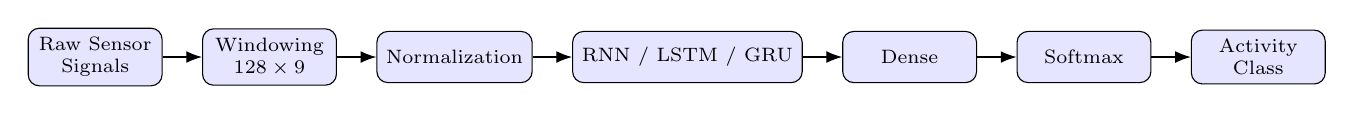
\begin{tikzpicture}[node distance=5mm]
\node[layer](a){Raw Sensor\\Signals};
\node[layer,right=of a](b){Windowing\\$128\times9$};
\node[layer,right=of b](c){Normalization};
\node[layer,right=of c](d){RNN / LSTM / GRU};
\node[layer,right=of d](e){Dense};
\node[layer,right=of e](f){Softmax};
\node[layer,right=of f](g){Activity\\Class};

\foreach \x/\y in {a/b,b/c,c/d,d/e,e/f,f/g}
\draw[arrow](\x)--(\y);
\end{tikzpicture}
\end{center}

The three recurrent models must use the same input, output layer, optimizer,
batch size and evaluation protocol.

%%%%%%%%%%%%%%%%%%%%%%%%%%%%%%%%%%%%%%%%%%%%%%%%%%%%%%%%%%%%
\section*{5. Preprocessing}

Perform the following preprocessing steps:

\begin{enumerate}
\item Load the raw inertial signals.
\item Arrange every observation window as $128\times9$.
\item Assign one activity label to each window.
\item Encode the six activity labels.
\item Normalize the input using statistics calculated from the training data.
\item Create training, validation and test sets.
\item Verify the class distribution.
\end{enumerate}

\textbf{Suggested split:}

\[
70\% \text{ training},\qquad
15\% \text{ validation},\qquad
15\% \text{ testing}.
\]

The test data must not be used during model selection or hyperparameter tuning.

\subsection*{Preprocessing Output}

A class-balanced subset of $N=3000$ windows (21 subjects) was used, with a
\emph{subject-wise} 70/15/15 split (train subjects
$\{5,6,7,11,14,16,17,19,21,22,23,26,28,29,30\}$, validation subjects
$\{3,8,15\}$, test subjects $\{1,25,27\}$) so that no subject appears in two
partitions.

\begin{verbatim}
Input tensor shape:
Training   : (2147, 128, 9)
Validation : (386, 128, 9)
Testing    : (467, 128, 9)

Number of classes: 6
Number of features per time step: 9
Sequence length: 128
\end{verbatim}

\textbf{Class distribution:}

\begin{center}
\begin{tabular}{|l|c|c|c|}
\hline
Activity & Train & Validation & Test\\
\hline
WALKING & 342 & 65 & 93\\
WALKING\_UPSTAIRS & 352 & 68 & 80\\
WALKING\_DOWNSTAIRS & 358 & 65 & 77\\
SITTING & 368 & 61 & 71\\
STANDING & 363 & 61 & 76\\
LAYING & 364 & 66 & 70\\
\hline
TOTAL & 2147 & 386 & 467\\
\hline
\end{tabular}
\end{center}

Class representation is approximately balanced in every split, confirming
that the subsetting and subject-wise split preserved all six classes.

%%%%%%%%%%%%%%%%%%%%%%%%%%%%%%%%%%%%%%%%%%%%%%%%%%%%%%%%%%%%
\section*{6. Temporal Data Visualization}

\begin{figure}[H]
\centering
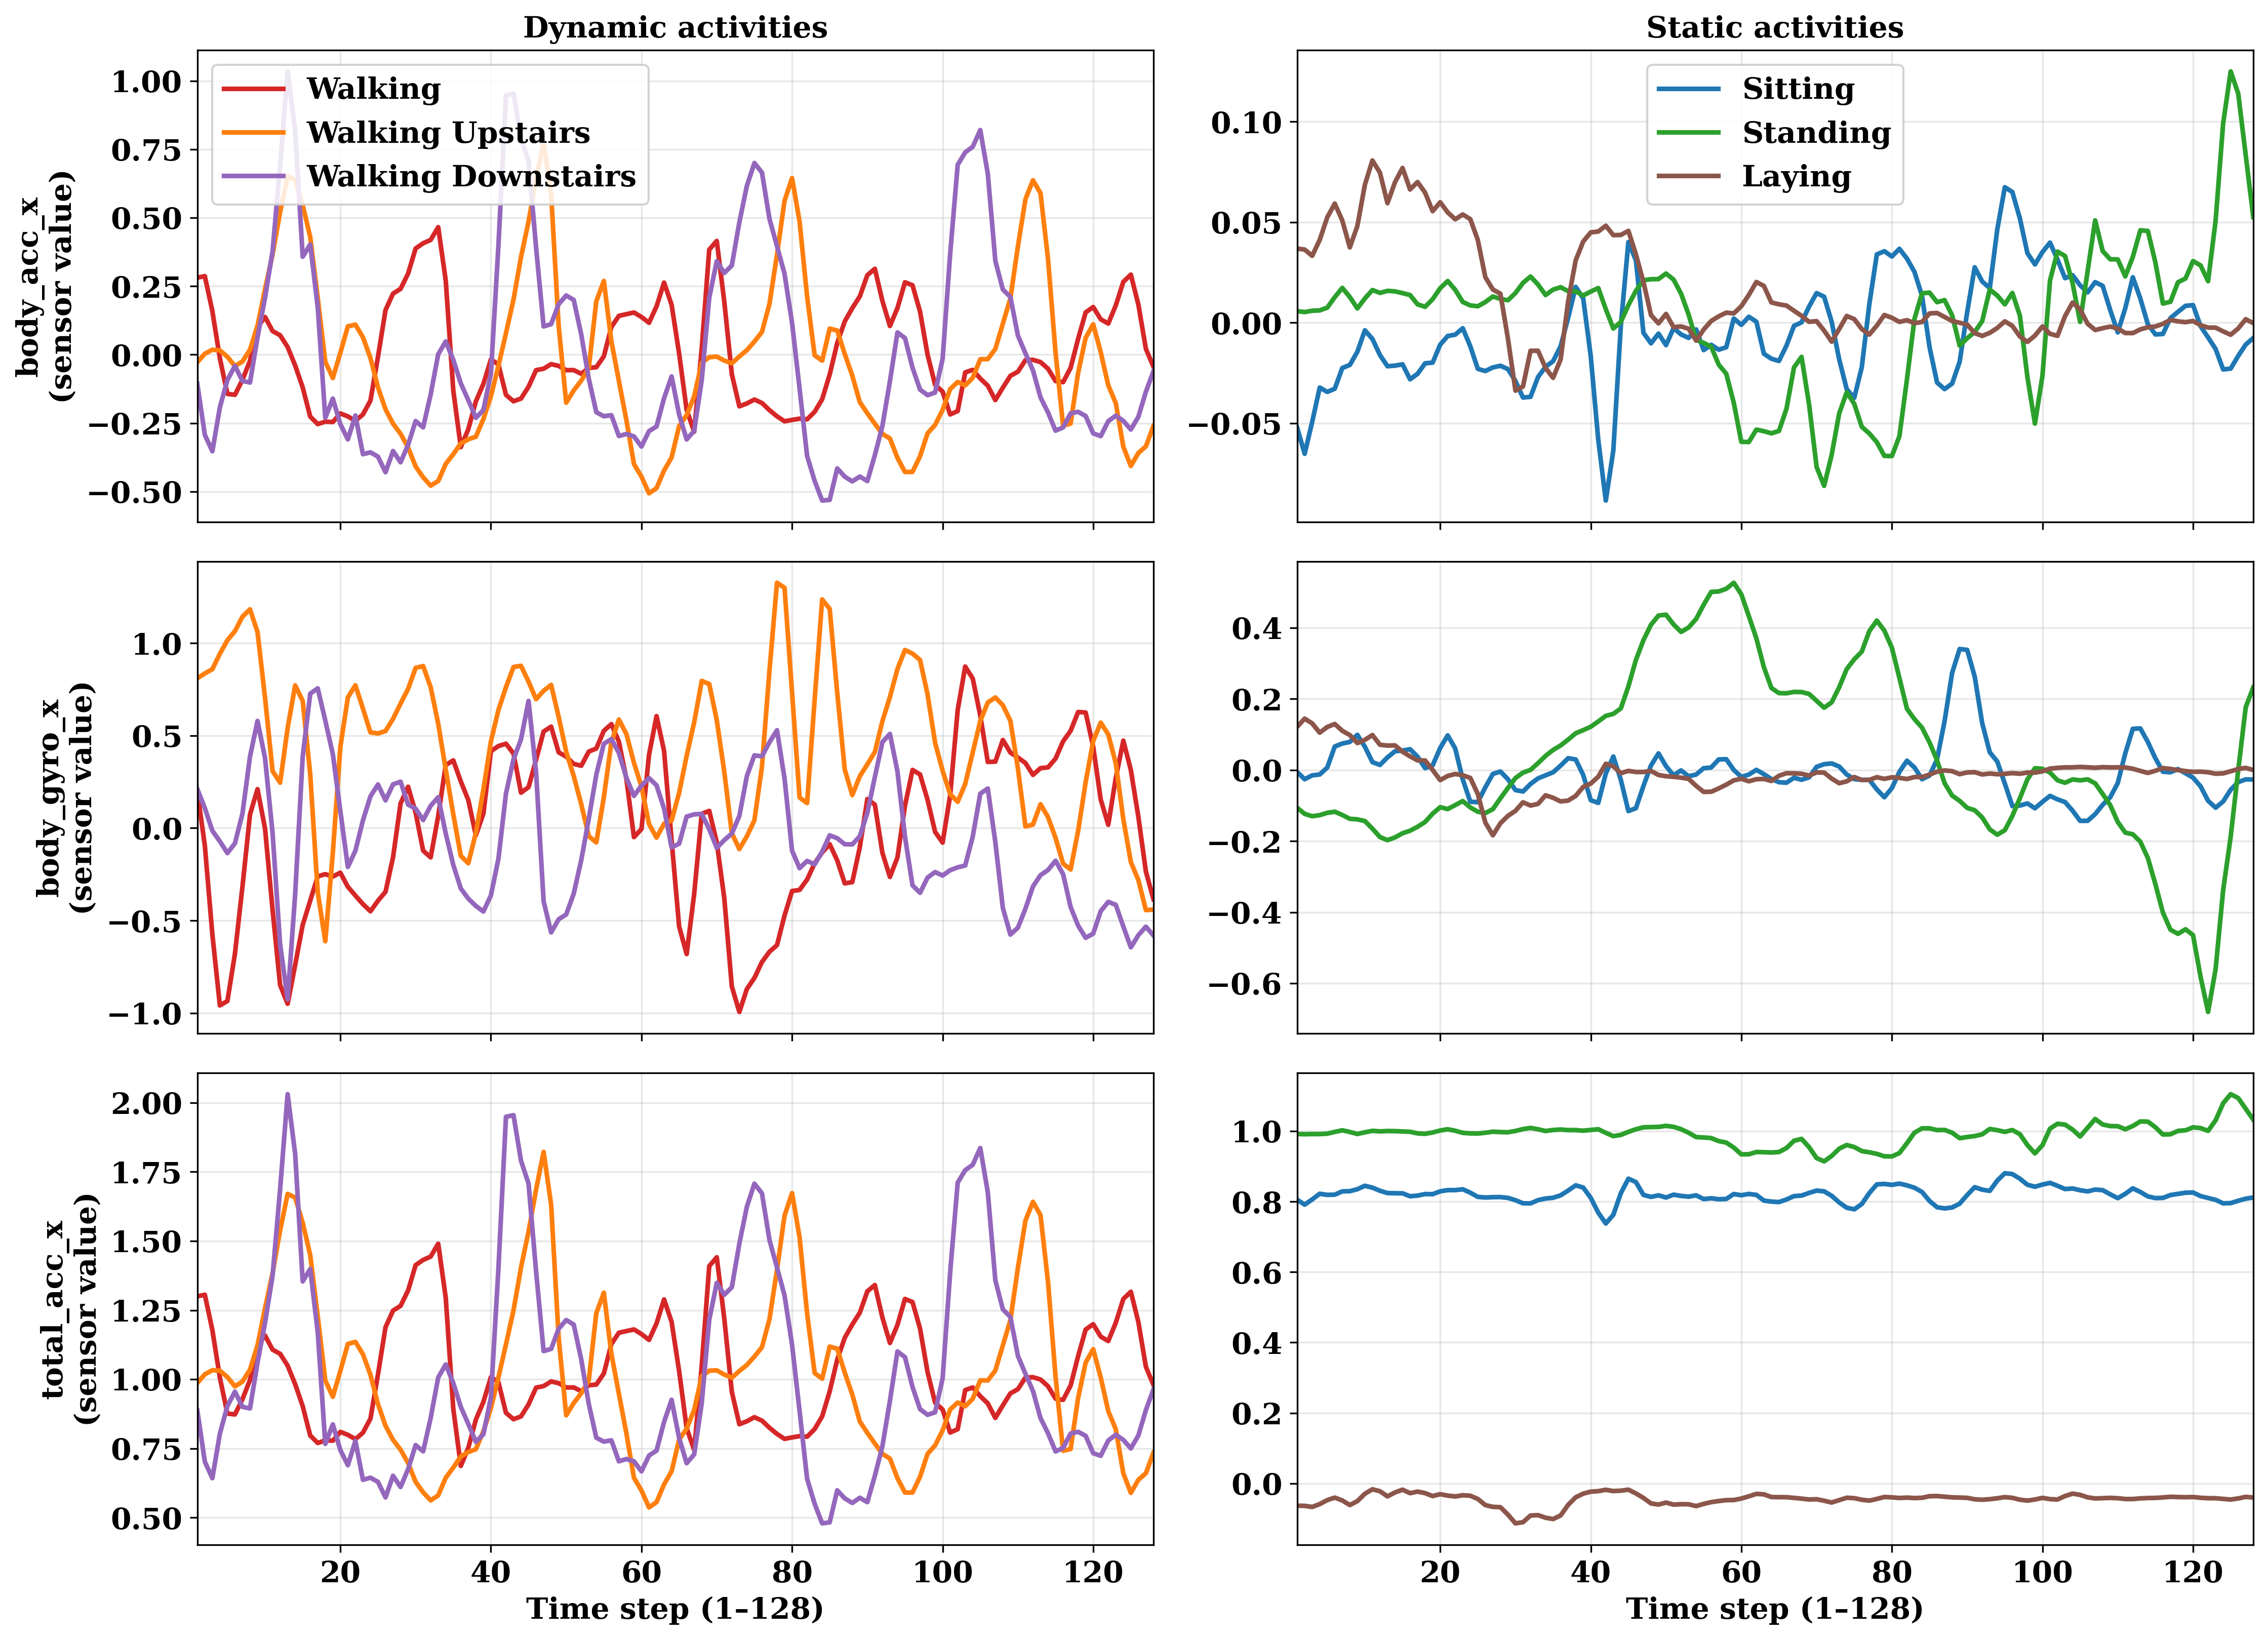
\includegraphics[width=0.95\textwidth]{plot01_sensor_signals.png}
\caption{Plot 1: body\_acc\_x, body\_gyro\_x and total\_acc\_x versus time step for the three dynamic activities (left) and three static activities (right).}
\end{figure}

\textbf{Inference:} Dynamic activities oscillate (body\_acc\_x std $0.29$ vs
$0.01$ for static activities); the most similar pair is Sitting \& Standing.
Order matters: gait cycles and posture changes exist only along time;
shuffling the steps destroys them.

%%%%%%%%%%%%%%%%%%%%%%%%%%%%%%%%%%%%%%%%%%%%%%%%%%%%%%%%%%%%
\section*{7. Vanilla RNN Architecture}

A Vanilla RNN maintains a hidden state that is updated at every time step:

\[
h_t=\tanh(W_xx_t+W_hh_{t-1}+b_h).
\]

The output can be written as

\[
y_t=g(W_yh_t+b_y).
\]

For sequence classification, the final hidden representation can be passed
to a classifier.

\begin{center}
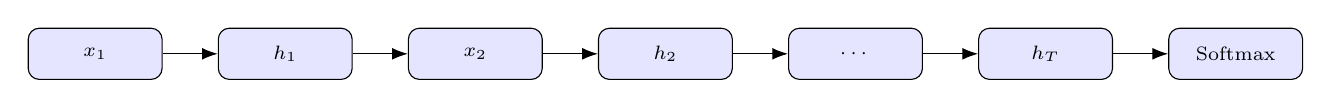
\begin{tikzpicture}[node distance=7mm]
\node[layer](x1){$x_1$};
\node[layer,right=of x1](h1){$h_1$};
\node[layer,right=of h1](x2){$x_2$};
\node[layer,right=of x2](h2){$h_2$};
\node[layer,right=of h2](x3){$\cdots$};
\node[layer,right=of x3](h3){$h_T$};
\node[layer,right=of h3](y){Softmax};

\draw[arrow](x1)--(h1);
\draw[arrow](h1)--(x2);
\draw[arrow](x2)--(h2);
\draw[arrow](h2)--(x3);
\draw[arrow](x3)--(h3);
\draw[arrow](h3)--(y);
\end{tikzpicture}
\end{center}

The diagram represents the unrolled view of an RNN. The same recurrent weights
are reused across time steps.

%%%%%%%%%%%%%%%%%%%%%%%%%%%%%%%%%%%%%%%%%%%%%%%%%%%%%%%%%%%%
\section*{8. Backpropagation Through Time}

When an RNN is unrolled, the loss depends on the sequence of hidden states.
Backpropagation Through Time (BPTT) propagates the error backward through
the recurrent steps.

\begin{center}
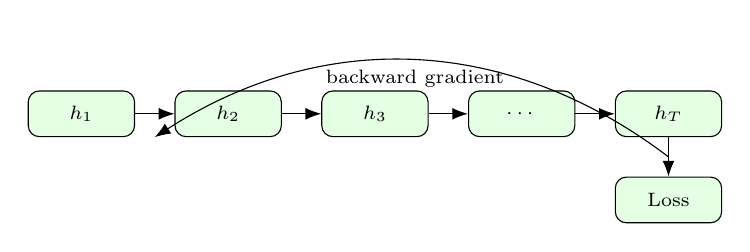
\begin{tikzpicture}[node distance=5mm]
\node[smalllayer](a){$h_1$};
\node[smalllayer,right=of a](b){$h_2$};
\node[smalllayer,right=of b](c){$h_3$};
\node[smalllayer,right=of c](d){$\cdots$};
\node[smalllayer,right=of d](e){$h_T$};
\node[smalllayer,below=of e](l){Loss};

\draw[arrow](a)--(b);
\draw[arrow](b)--(c);
\draw[arrow](c)--(d);
\draw[arrow](d)--(e);
\draw[arrow](e)--(l);

\draw[arrow]($(e.south)!0.5!(l.north)$) to[bend right=35]
node[below,font=\scriptsize]{backward gradient} ($(a.south)!0.5!(b.south)$);
\end{tikzpicture}
\end{center}

Students should explain that repeated multiplication of derivatives through
many time steps can cause gradients to become extremely small or extremely
large.

\subsection*{Challenges}

\begin{itemize}
\item Vanishing gradients
\item Exploding gradients
\item Difficulty learning long-term dependencies
\item Sequential computation and limited parallelism
\end{itemize}

The vanishing-gradient problem can be conceptually represented as

\[
\left|\frac{\partial h_t}{\partial h_{t-k}}\right|\rightarrow0
\]

while exploding gradients correspond to very large gradient magnitudes.

\subsection*{Numerical Exercise}

Consider

\[
x_1=0.5,\qquad x_2=0.7,\qquad x_3=0.2,
\]

\[
h_0=0,\qquad W_x=0.5,\qquad W_h=0.8,\qquad b=0.1.
\]

Using

\[
h_t=\tanh(W_xx_t+W_hh_{t-1}+b),
\]

calculate $h_1$, $h_2$ and $h_3$ manually.

Students must compare their calculated values with the values obtained from
a program.

\subsection*{Observed Results}

\begin{center}
\begin{tabular}{|c|c|c|c|c|}
\hline
Step & Manual (4 d.p.) & NumPy & Keras SimpleRNN & $|\text{NumPy}-\text{Manual}|$\\
\hline
$h_1$ & 0.3364 & 0.336376 & 0.336376 & 0.000024\\
$h_2$ & 0.6164 & 0.616352 & 0.616352 & 0.000048\\
$h_3$ & 0.6000 & 0.599958 & 0.599958 & 0.000042\\
\hline
\end{tabular}
\end{center}

\textbf{Inference:} Manual, NumPy and Keras agree: $h=[0.3364,\,0.6164,\,0.6000]$
(max difference $5\times10^{-5}$, from 4-d.p.\ rounding). The same
$W_x,\,W_h,\,b$ are reused at every step; only the hidden state carries the
past forward.

%%%%%%%%%%%%%%%%%%%%%%%%%%%%%%%%%%%%%%%%%%%%%%%%%%%%%%%%%%%%
\section*{9. RNN Implementation}

Use a small recurrent architecture:

\begin{center}
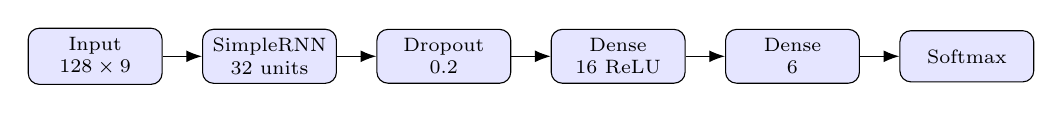
\begin{tikzpicture}[node distance=5mm]
\node[layer](a){Input\\$128\times9$};
\node[layer,right=of a](b){SimpleRNN\\32 units};
\node[layer,right=of b](c){Dropout\\0.2};
\node[layer,right=of c](d){Dense\\16 ReLU};
\node[layer,right=of d](e){Dense\\6};
\node[layer,right=of e](f){Softmax};

\foreach \x/\y in {a/b,b/c,c/d,d/e,e/f}
\draw[arrow](\x)--(\y);
\end{tikzpicture}
\end{center}

\textbf{Suggested training configuration:}

\begin{center}
\begin{tabular}{|l|l|}
\hline
Parameter & Value\\
\hline
Recurrent units & 32\\
Dropout & 0.2\\
Optimizer & Adam\\
Learning rate & $10^{-3}$\\
Batch size & 32\\
Epochs & 30\\
Loss & Sparse categorical cross-entropy\\
\hline
\end{tabular}
\end{center}

\subsection*{Observed Results}

The RNN model (\texttt{SimpleRNN(32)}) has 1{,}974 trainable parameters. With
the configuration above (Adam, lr $10^{-3}$, batch 32, 30 epochs) and the
best-validation-loss epoch restored:

\begin{verbatim}
epoch   1 | loss 1.6319  acc  36.4% | val_loss 1.4551  val_acc  45.6%
epoch   5 | loss 1.0377  acc  53.2% | val_loss 1.2108  val_acc  47.2%
epoch  10 | loss 0.8852  acc  59.0% | val_loss 0.7798  val_acc  67.1%
epoch  15 | loss 0.7223  acc  65.8% | val_loss 0.6614  val_acc  71.0%
epoch  20 | loss 0.6667  acc  69.7% | val_loss 0.6225  val_acc  69.2%
epoch  25 | loss 0.6332  acc  71.3% | val_loss 0.6163  val_acc  71.5%
epoch  30 | loss 0.6169  acc  73.0% | val_loss 0.5770  val_acc  72.8%

==> RNN: test accuracy 72.16% | macro-F1 73.03% | parameters 1,974
    | training time 30.6 s | best epoch 28/30
\end{verbatim}

%%%%%%%%%%%%%%%%%%%%%%%%%%%%%%%%%%%%%%%%%%%%%%%%%%%%%%%%%%%%
\section*{10. LSTM Architecture}

LSTM introduces a memory cell and gates to control information flow.

The forget gate is

\[
f_t=\sigma(W_f[h_{t-1},x_t]+b_f),
\]

the input gate is

\[
i_t=\sigma(W_i[h_{t-1},x_t]+b_i),
\]

and the output gate is

\[
o_t=\sigma(W_o[h_{t-1},x_t]+b_o).
\]

The candidate cell state is

\[
\tilde{C}_t=
\tanh(W_C[h_{t-1},x_t]+b_C),
\]

and the cell state is

\[
C_t=f_tC_{t-1}+i_t\tilde{C}_t.
\]

The hidden state is

\[
h_t=o_t\tanh(C_t).
\]

\begin{center}
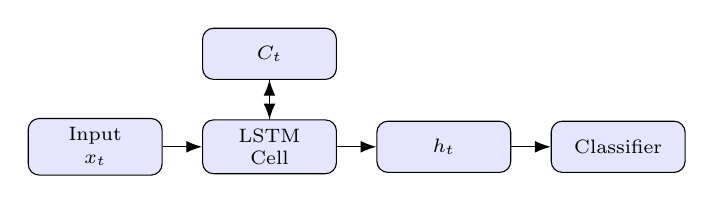
\begin{tikzpicture}[node distance=5mm]
\node[layer](a){Input\\$x_t$};
\node[layer,right=of a](b){LSTM\\Cell};
\node[layer,right=of b](c){$h_t$};
\node[layer,above=of b](d){$C_t$};
\node[layer,right=of c](e){Classifier};

\draw[arrow](a)--(b);
\draw[arrow](b)--(c);
\draw[arrow](b)--(d);
\draw[arrow](c)--(e);
\draw[arrow](d)--(b);
\end{tikzpicture}
\end{center}


\textbf{Inference:} $C_t=f_t\odot C_{t-1}+i_t\odot\tilde{C}_t$ is an additive
path: $f_t\approx1$ keeps memory, $f_t\approx0$ discards it. The input gate
writes new evidence; the output gate decides how much memory is exposed as
$h_t$.

%%%%%%%%%%%%%%%%%%%%%%%%%%%%%%%%%%%%%%%%%%%%%%%%%%%%%%%%%%%%
\section*{11. GRU Architecture}

GRU uses two principal gates:

\[
z_t=\sigma(W_z[h_{t-1},x_t]+b_z)
\]

and

\[
r_t=\sigma(W_r[h_{t-1},x_t]+b_r).
\]

The candidate hidden state is

\[
\tilde{h}_t=
\tanh(W_h[r_t\odot h_{t-1},x_t]+b_h).
\]

The hidden state is updated using

\[
h_t=(1-z_t)h_{t-1}+z_t\tilde{h}_t.
\]

\begin{center}
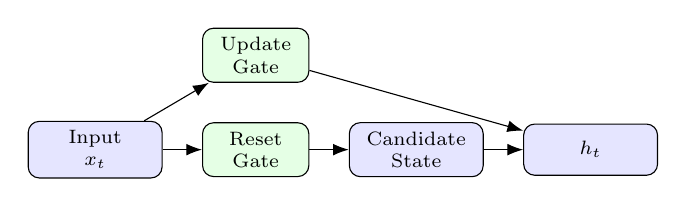
\begin{tikzpicture}[node distance=5mm]
\node[layer](a){Input\\$x_t$};
\node[smalllayer,right=of a](b){Reset\\Gate};
\node[smalllayer,above=of b](c){Update\\Gate};
\node[layer,right=of b](d){Candidate\\State};
\node[layer,right=of d](e){$h_t$};

\draw[arrow](a)--(b);
\draw[arrow](a)--(c);
\draw[arrow](b)--(d);
\draw[arrow](c)--(e);
\draw[arrow](d)--(e);
\end{tikzpicture}
\end{center}

Students should compare the number of gates and state representations in
RNN, LSTM and GRU.

\textbf{Inference:} RNN: 1 state, 0 gates $\cdot$ LSTM: $h$ and $C$, 3 gates
(forget, input, output) $\cdot$ GRU: 1 state, 2 gates (update, reset). The
update gate blends the old state and the candidate, giving a shorter
gradient path with fewer weights than LSTM.

%%%%%%%%%%%%%%%%%%%%%%%%%%%%%%%%%%%%%%%%%%%%%%%%%%%%%%%%%%%%
\section*{12. LSTM and GRU Implementation}

Implement the same classifier used for the RNN, replacing only the recurrent
layer.

\begin{center}
\begin{tabular}{|l|c|c|c|}
\hline
Model & Recurrent Layer & Units & Output Classes\\
\hline
RNN & SimpleRNN & 32 & 6\\
LSTM & LSTM & 32 & 6\\
GRU & GRU & 32 & 6\\
\hline
\end{tabular}
\end{center}

All other experimental conditions should remain unchanged.

\subsection*{Observed Results}

LSTM has 6{,}006 trainable parameters and GRU has 4{,}758, both trained with
the same Adam optimiser, batch size, epochs and loss as the RNN.

\begin{verbatim}
Training LSTM ...
epoch   1 | loss 1.5907  acc  34.7% | val_loss 1.3709  val_acc  40.2%
epoch   5 | loss 0.6550  acc  75.3% | val_loss 0.4717  val_acc  83.2%
epoch  10 | loss 0.2954  acc  88.9% | val_loss 0.2271  val_acc  93.0%
epoch  15 | loss 0.2079  acc  91.3% | val_loss 0.2099  val_acc  96.4%
epoch  20 | loss 0.2873  acc  89.6% | val_loss 0.4409  val_acc  87.0%
epoch  25 | loss 0.1351  acc  95.0% | val_loss 0.1465  val_acc  96.1%
epoch  30 | loss 0.1215  acc  95.1% | val_loss 0.1887  val_acc  95.9%
==> LSTM: test accuracy 94.86% | macro-F1 94.84% | parameters 6,006
    | training time 25.5 s | best epoch 25/30

Training GRU ...
epoch   1 | loss 1.6165  acc  35.7% | val_loss 1.4350  val_acc  45.1%
epoch   5 | loss 0.5860  acc  76.8% | val_loss 0.4273  val_acc  83.4%
epoch  10 | loss 0.2865  acc  89.1% | val_loss 0.1759  val_acc  96.9%
epoch  15 | loss 0.1822  acc  92.8% | val_loss 0.1111  val_acc  98.2%
epoch  20 | loss 0.1467  acc  94.0% | val_loss 0.1221  val_acc  97.4%
epoch  25 | loss 0.1472  acc  93.5% | val_loss 0.0895  val_acc  97.4%
epoch  30 | loss 0.1298  acc  94.6% | val_loss 0.1578  val_acc  96.4%
==> GRU: test accuracy 98.29% | macro-F1 98.29% | parameters 4,758
    | training time 26.3 s | best epoch 25/30
\end{verbatim}

%%%%%%%%%%%%%%%%%%%%%%%%%%%%%%%%%%%%%%%%%%%%%%%%%%%%%%%%%%%%
\section*{13. Required Training Plots}

\begin{figure}[H]
\centering
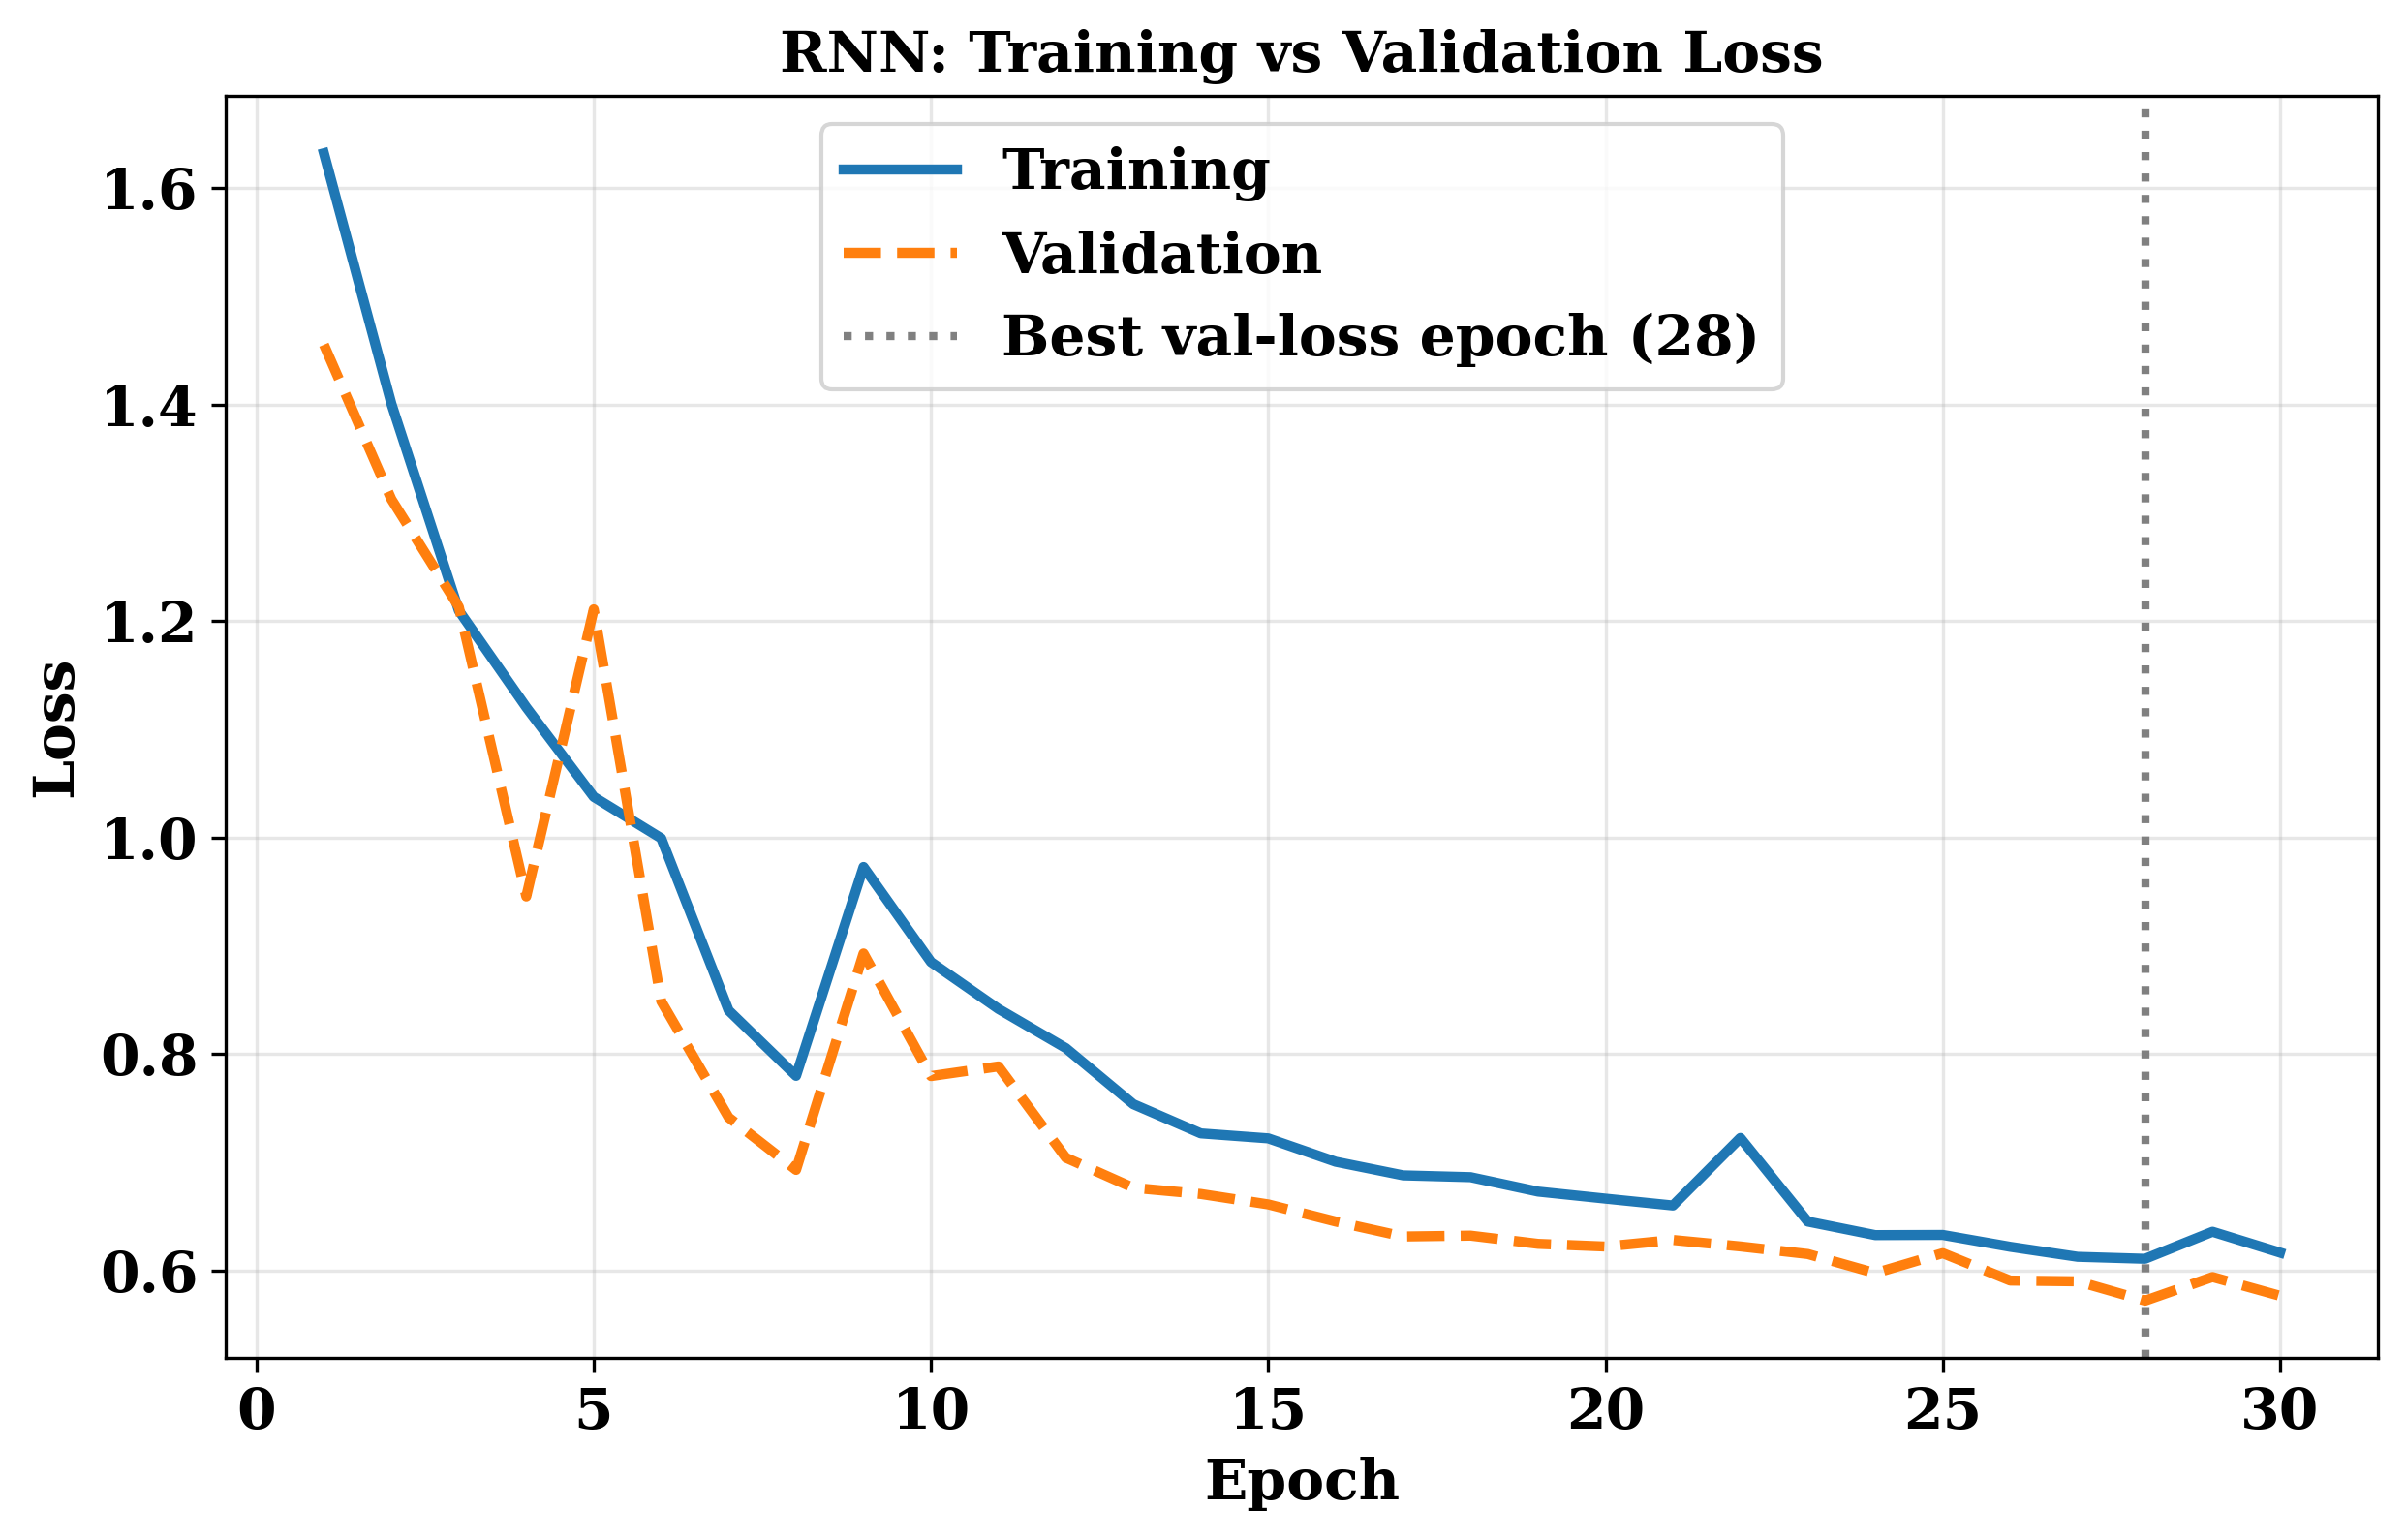
\includegraphics[width=0.48\textwidth]{plot02_loss_RNN.png}
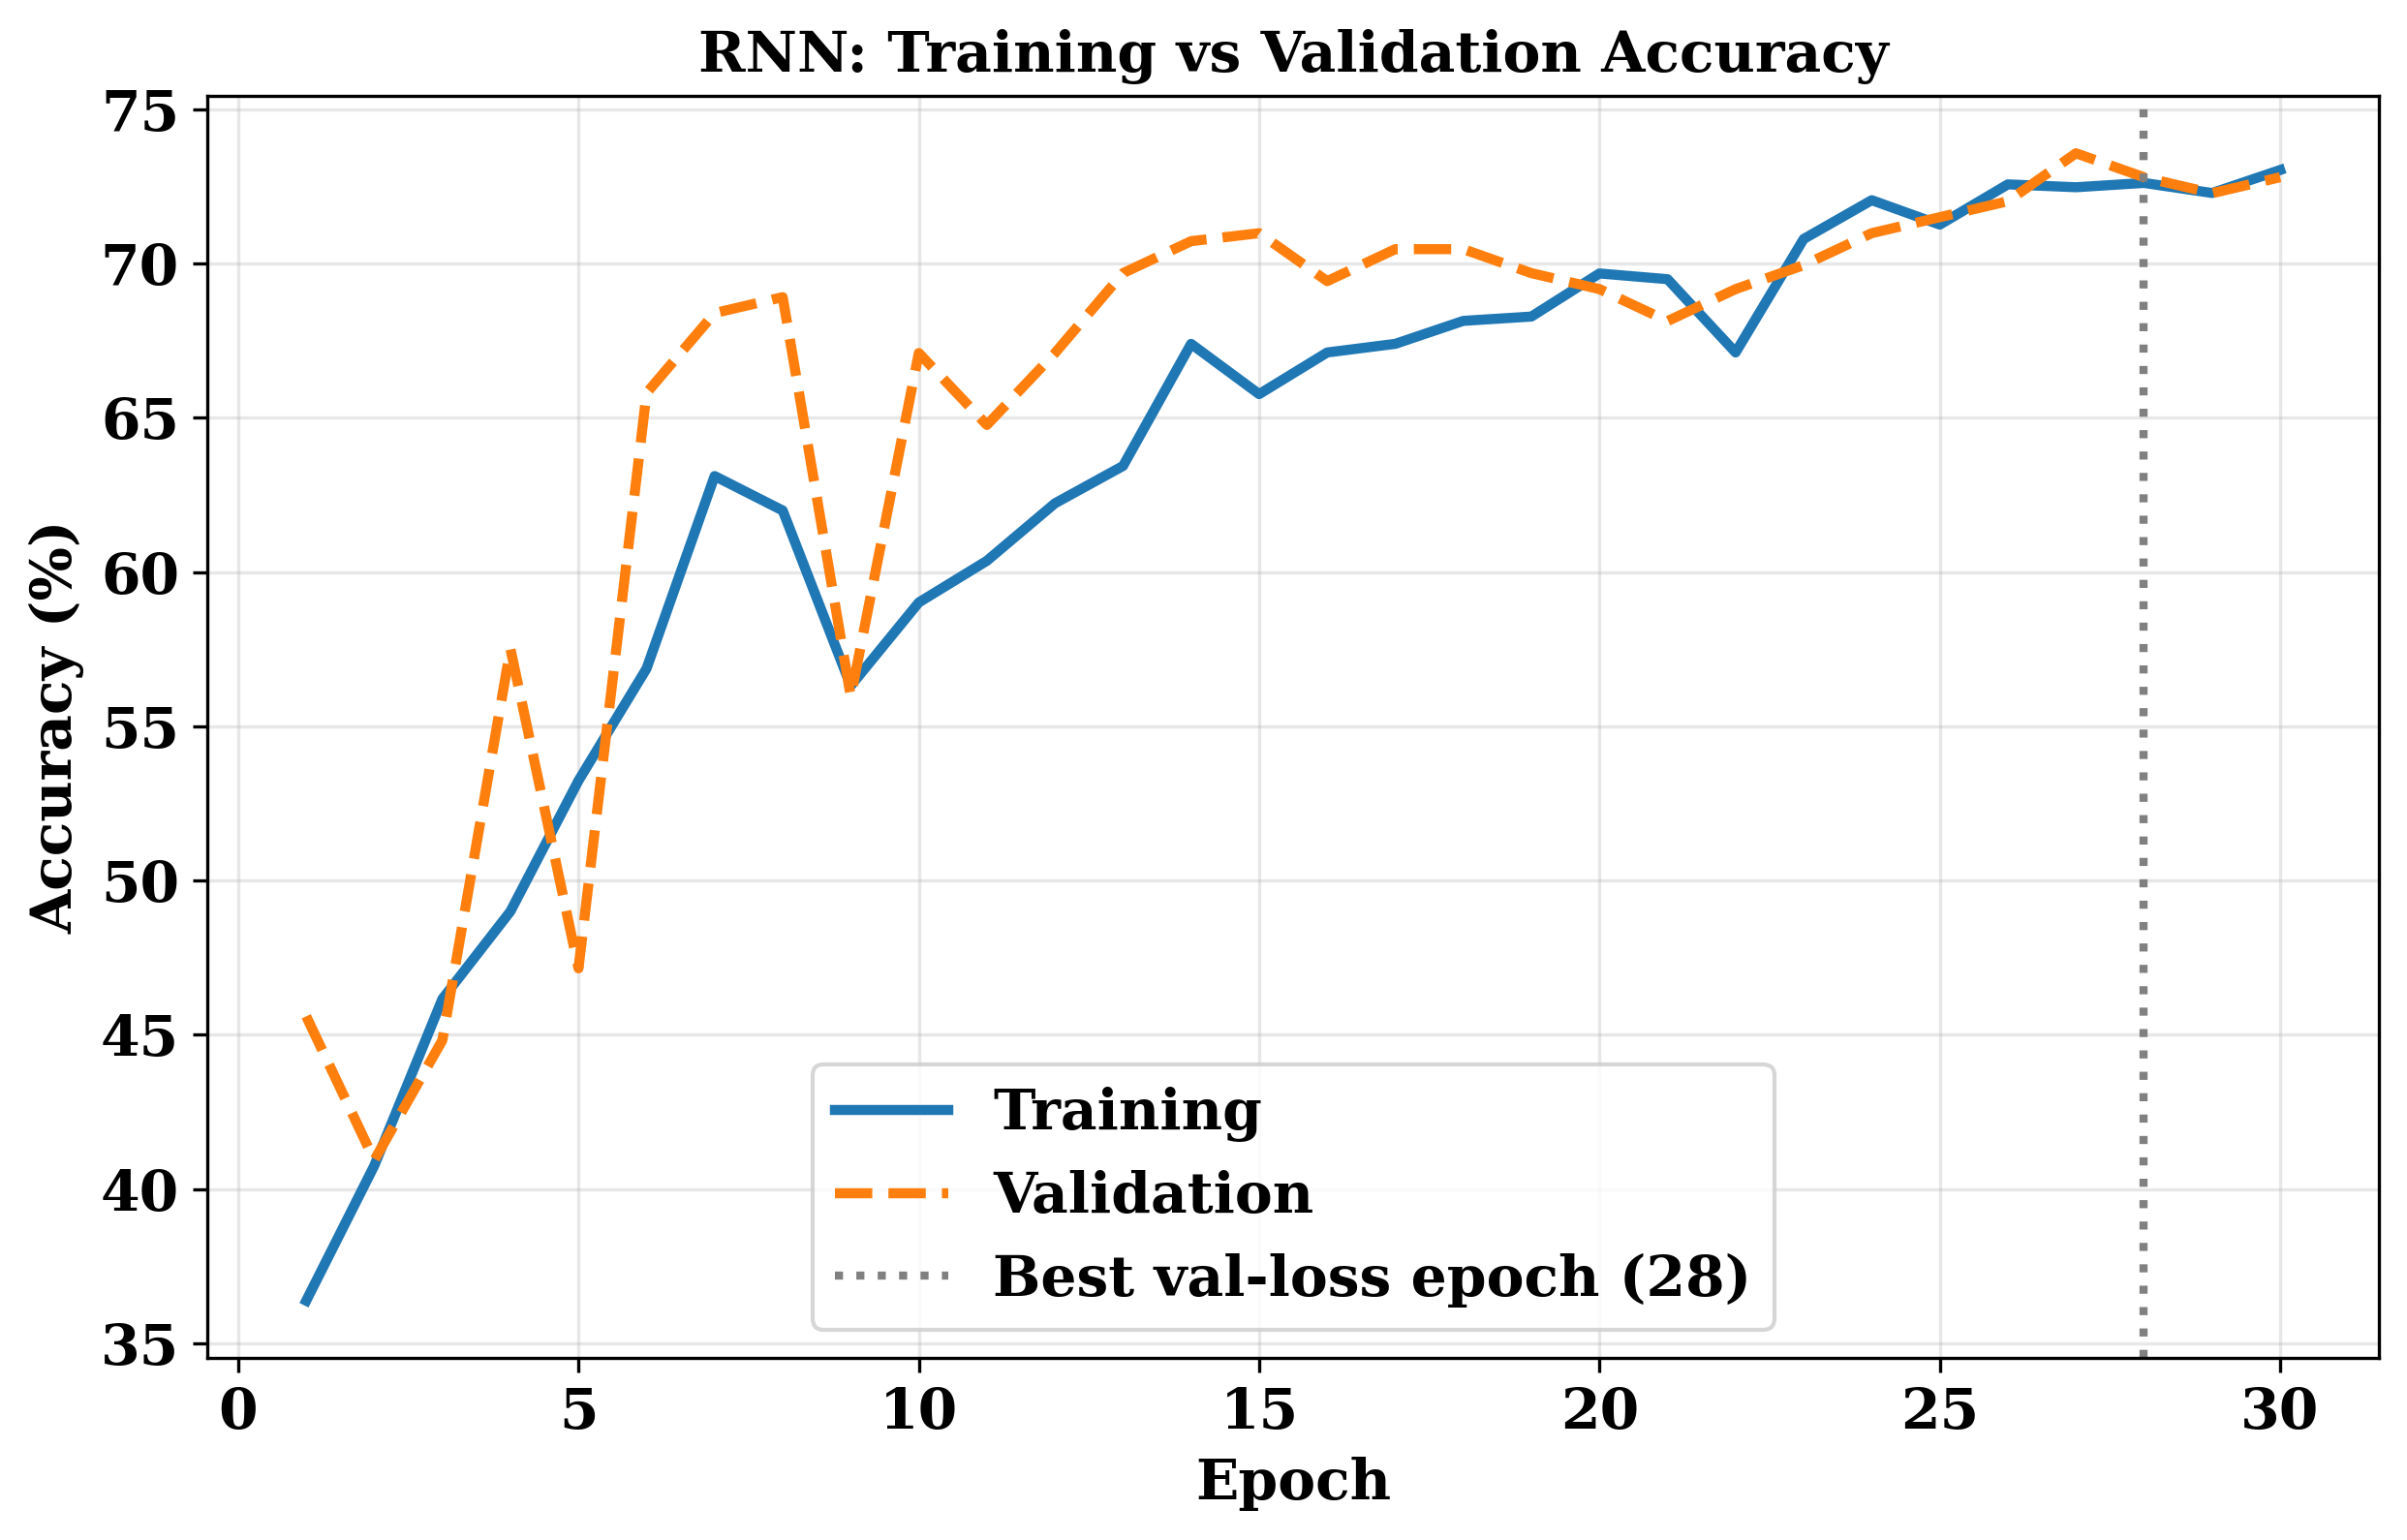
\includegraphics[width=0.48\textwidth]{plot03_accuracy_RNN.png}
\caption{RNN -- Plot 2 (training/validation loss) and Plot 3 (training/validation accuracy).}
\end{figure}

\textbf{Inference (loss):} RNN: train loss $1.63\rightarrow0.62$; val loss
minimum $0.57$ at epoch 28/30, within 5\% of it from epoch 24. Still
converging -- no gates, so gradients vanish over 128 steps.

\textbf{Inference (accuracy):} RNN: final train/val accuracy $73.0\%/72.8\%$
(best val $73.6\%$); gap $+0.2$ pts. Curves still improving $\rightarrow$
more epochs would likely help.

\begin{figure}[H]
\centering
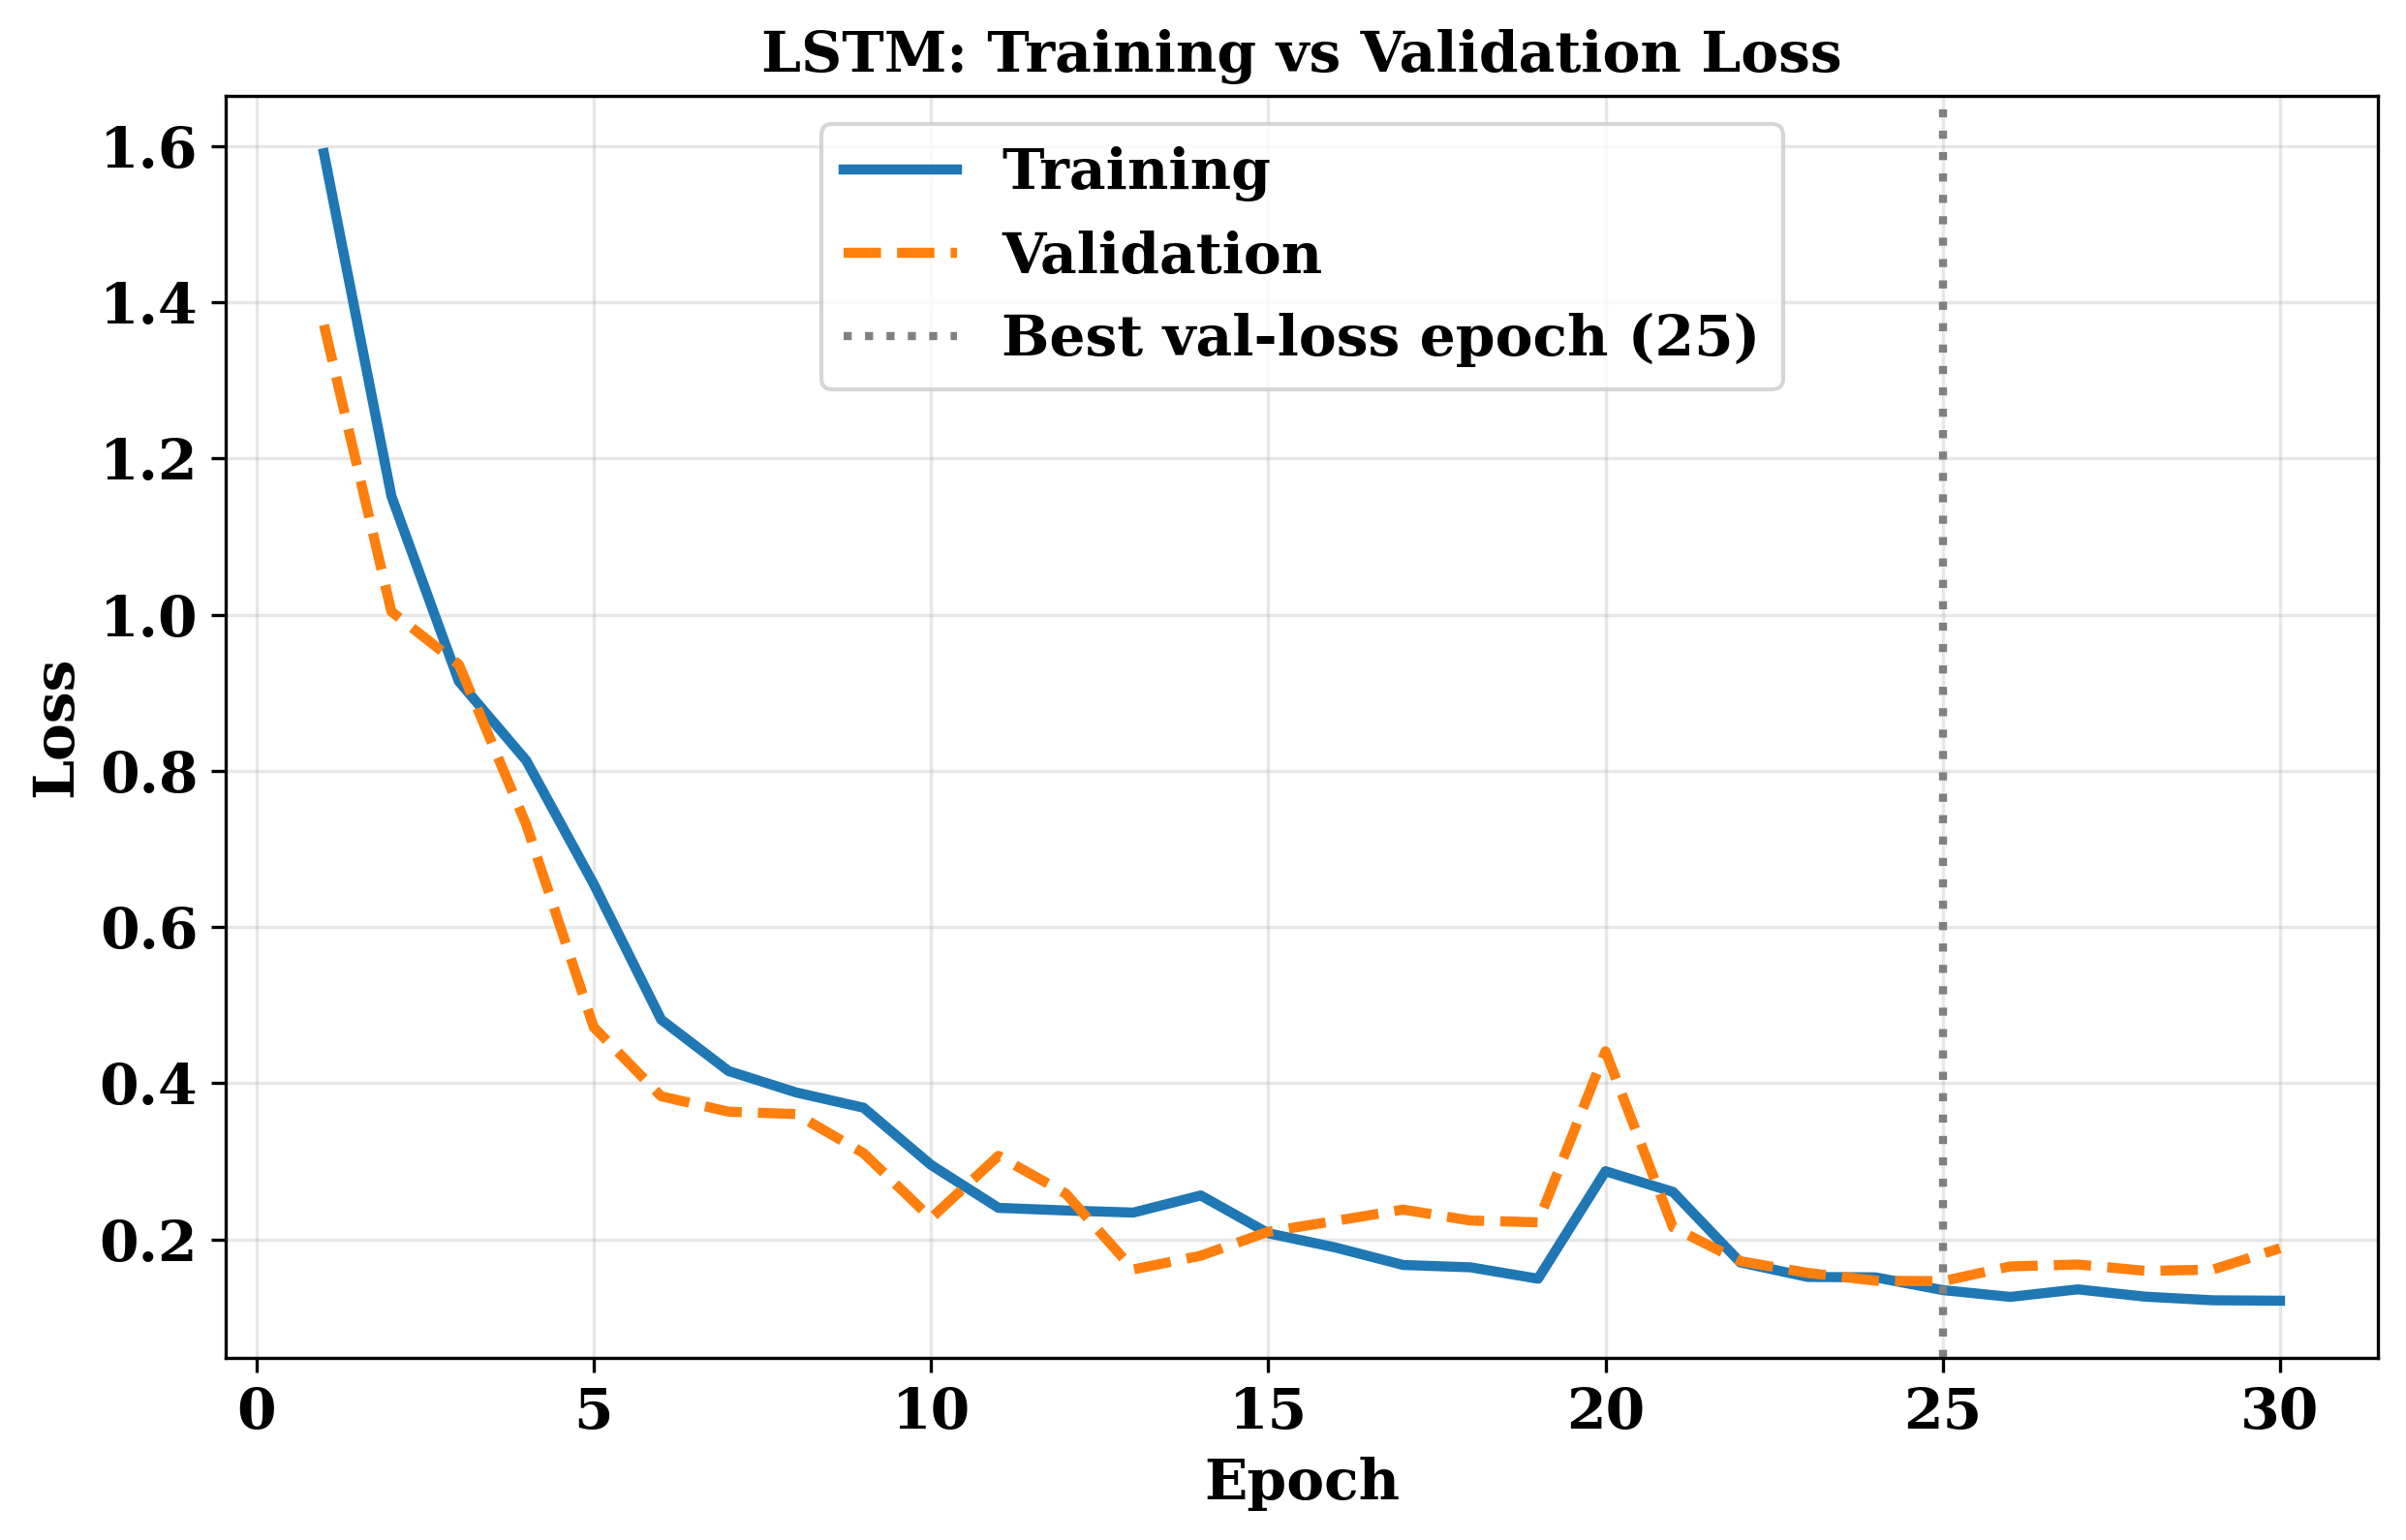
\includegraphics[width=0.48\textwidth]{plot02_loss_LSTM.png}
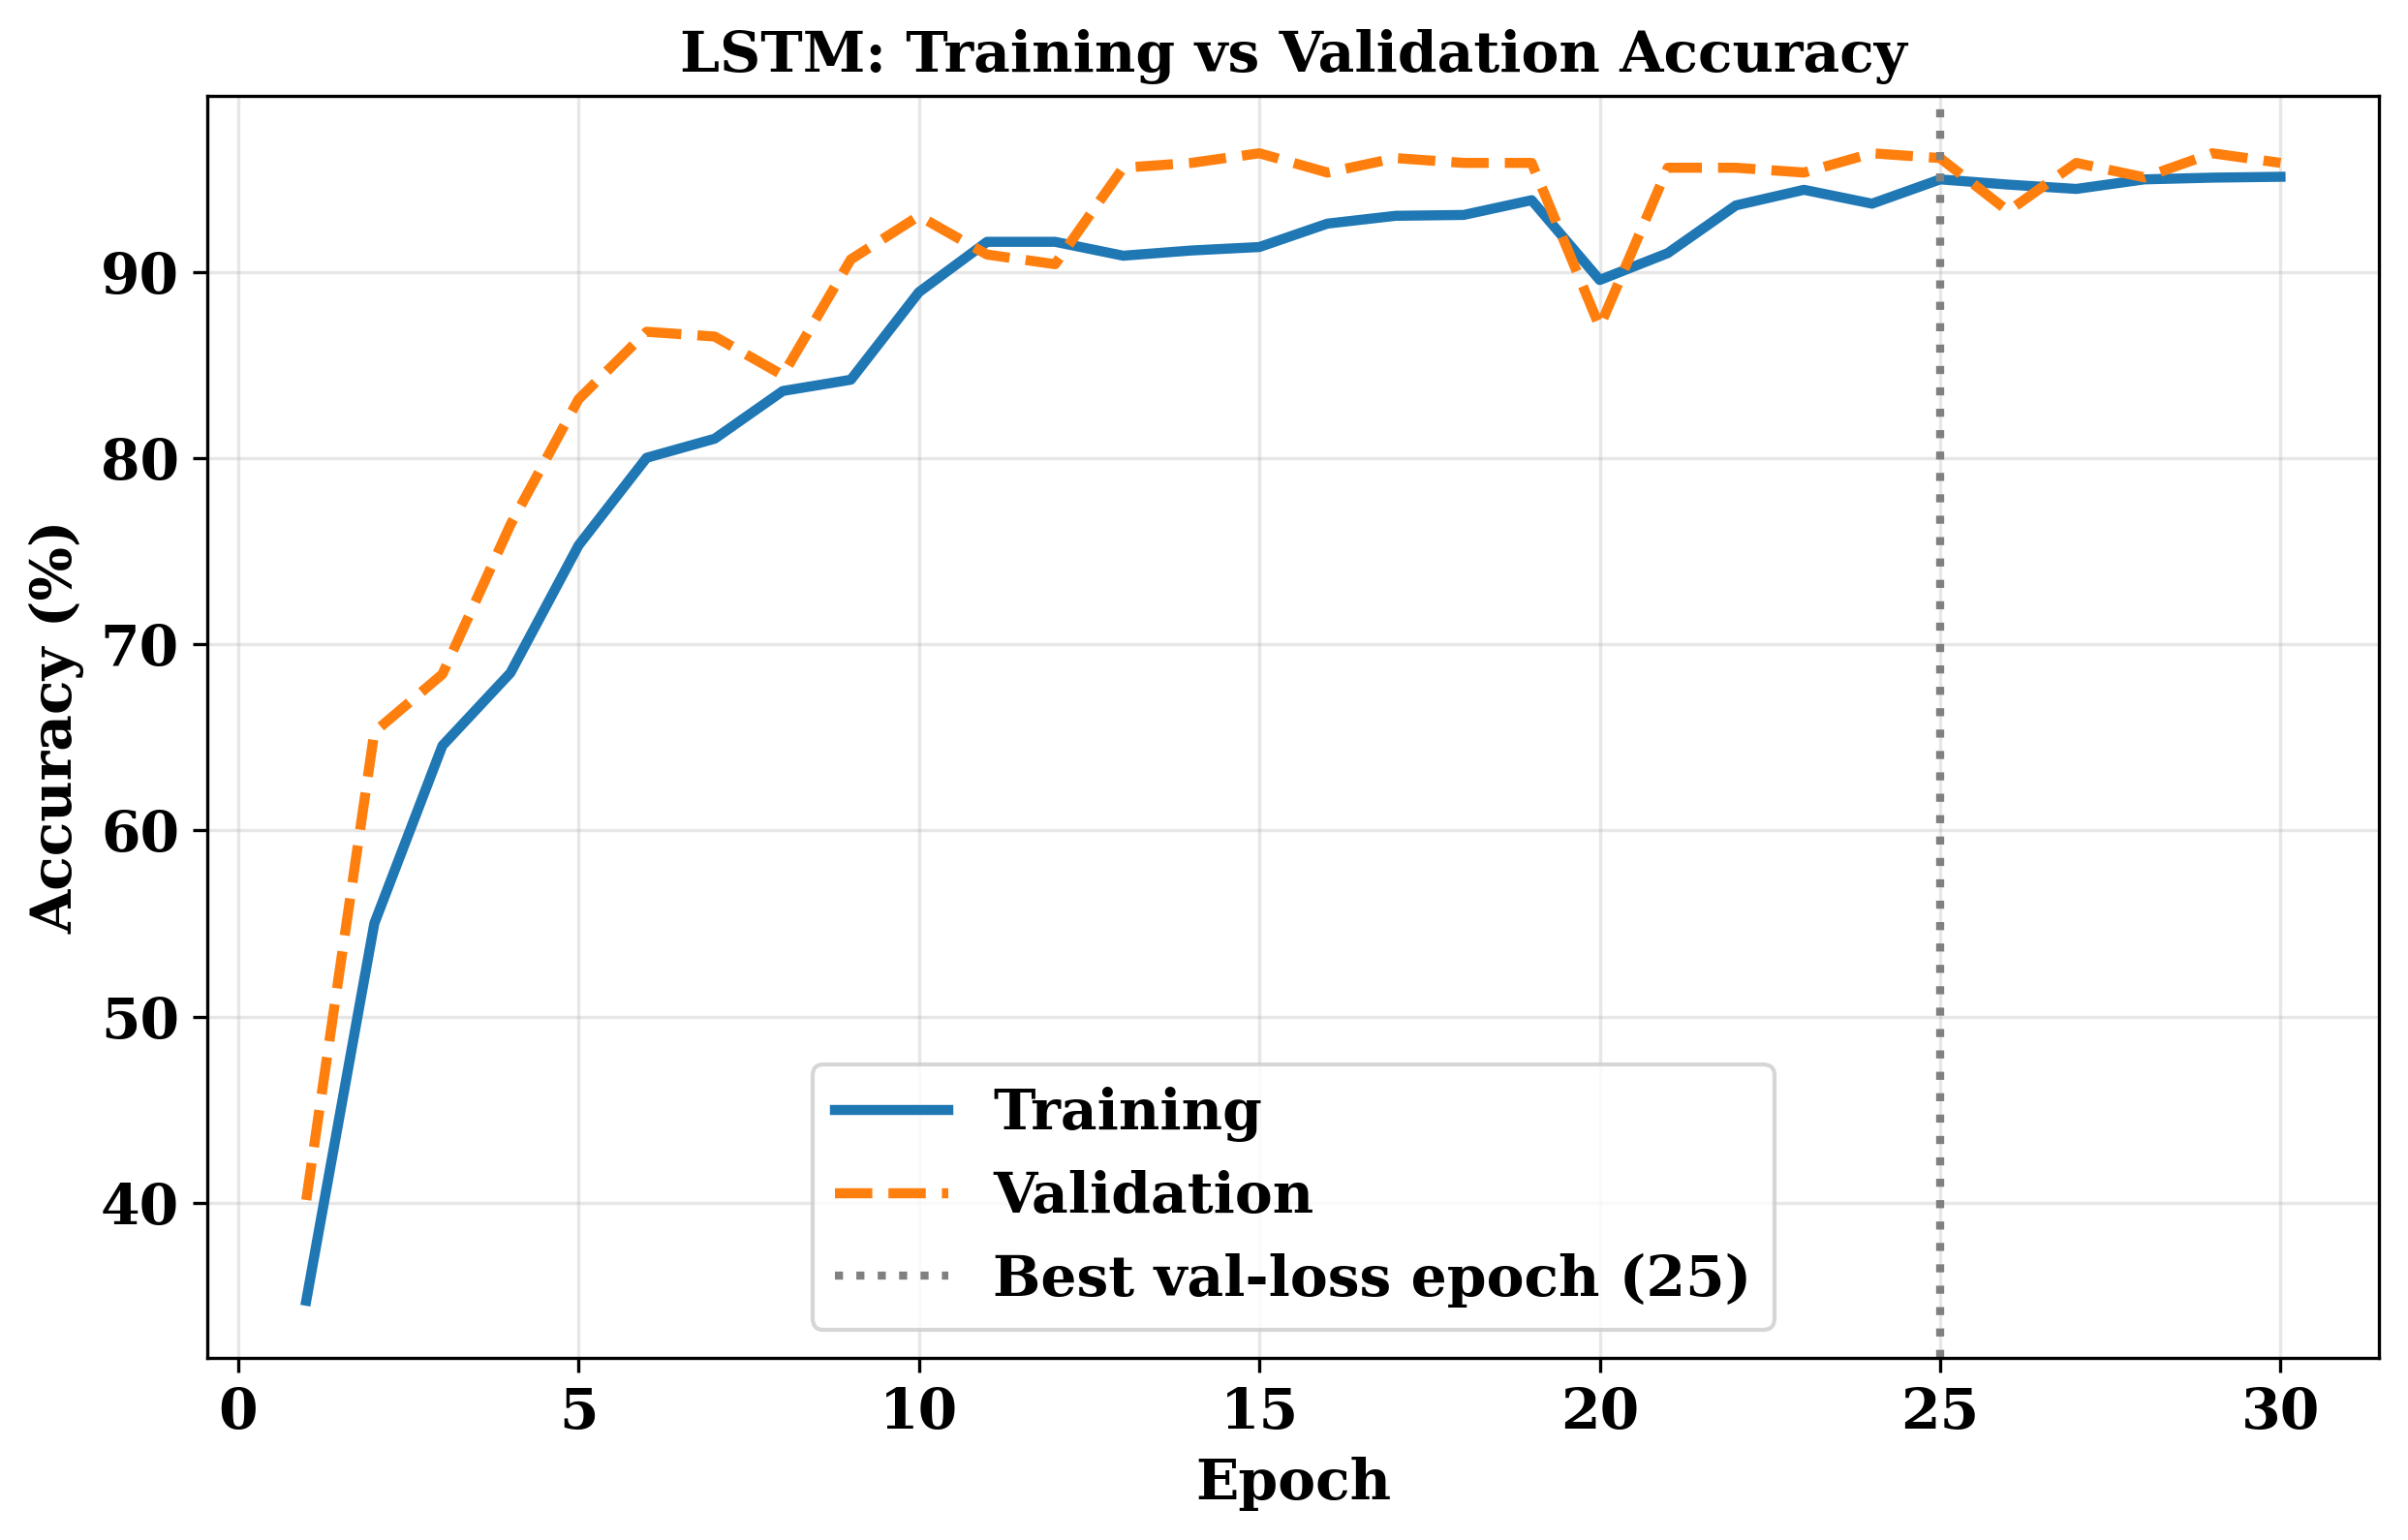
\includegraphics[width=0.48\textwidth]{plot03_accuracy_LSTM.png}
\caption{LSTM -- Plot 2 (training/validation loss) and Plot 3 (training/validation accuracy).}
\end{figure}

\textbf{Inference (loss):} LSTM: train loss $1.59\rightarrow0.12$; val loss
minimum $0.15$ at epoch 25/30, within 5\% of it from epoch 24. Converged,
small generalisation gap -- the gated cell state preserves gradients.

\textbf{Inference (accuracy):} LSTM: final train/val accuracy
$95.1\%/95.9\%$ (best val $96.4\%$); gap $-0.7$ pts. Train and val track
each other $\rightarrow$ generalises to unseen data.

\begin{figure}[H]
\centering
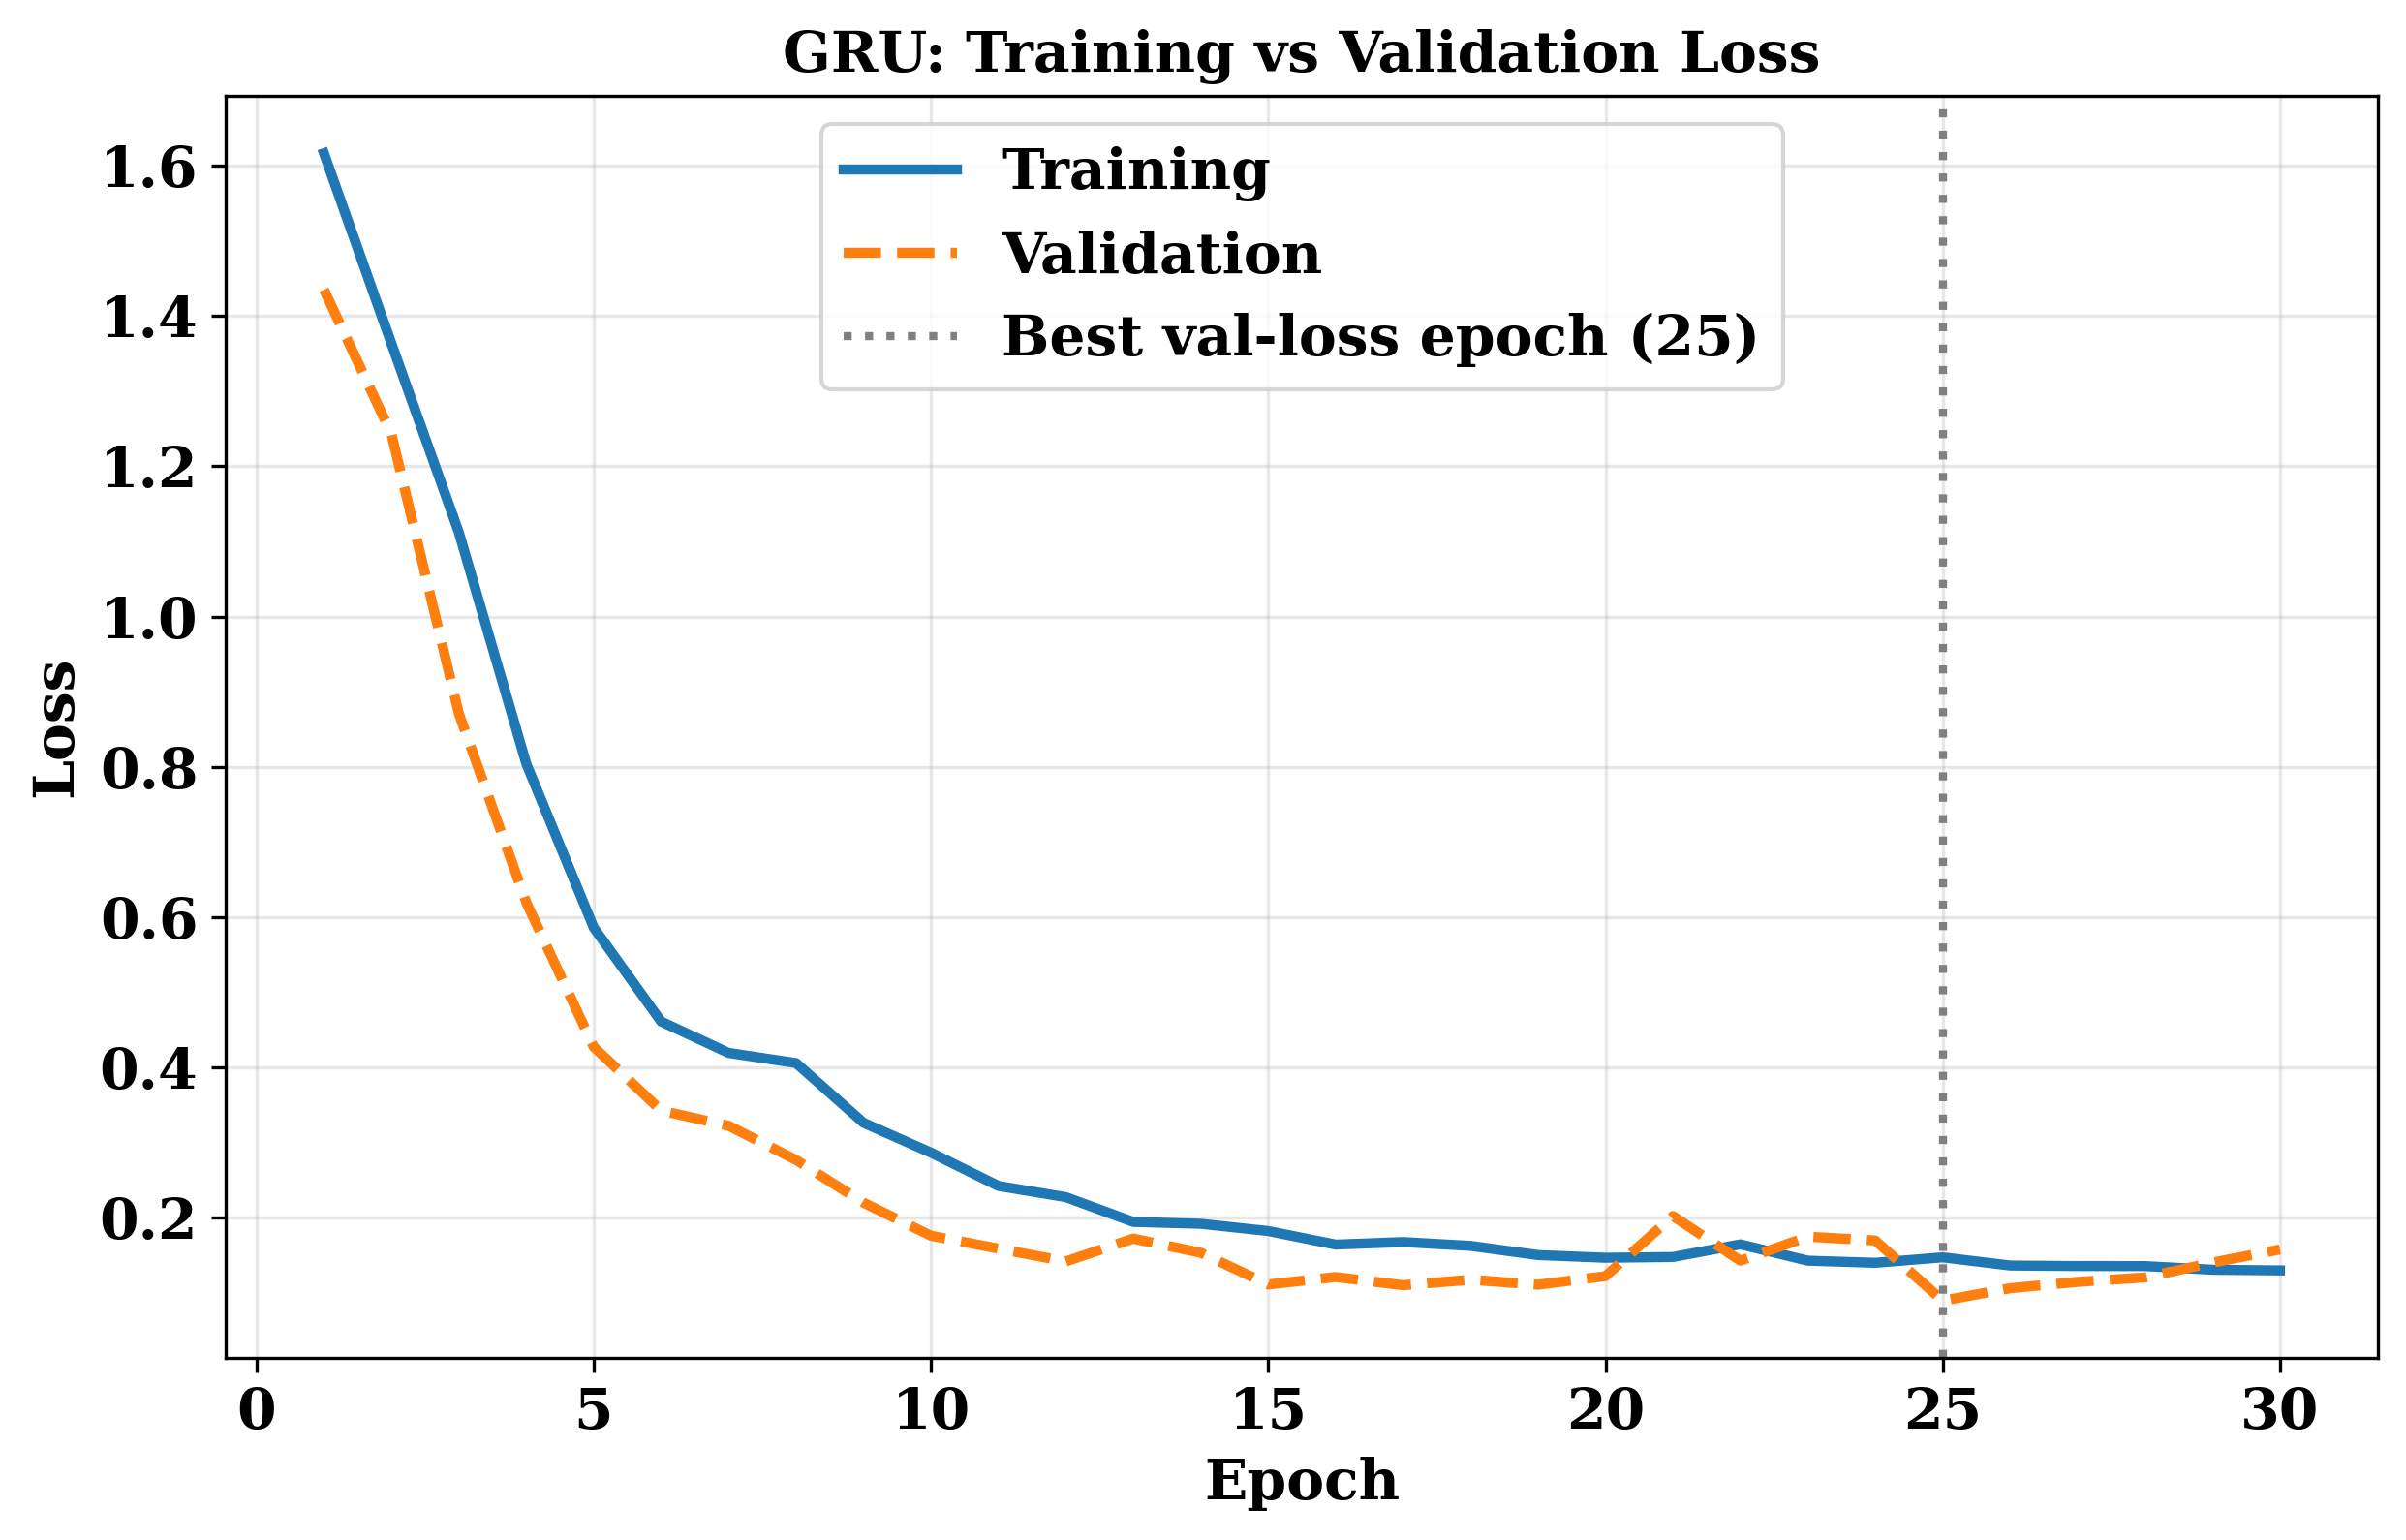
\includegraphics[width=0.48\textwidth]{plot02_loss_GRU.png}
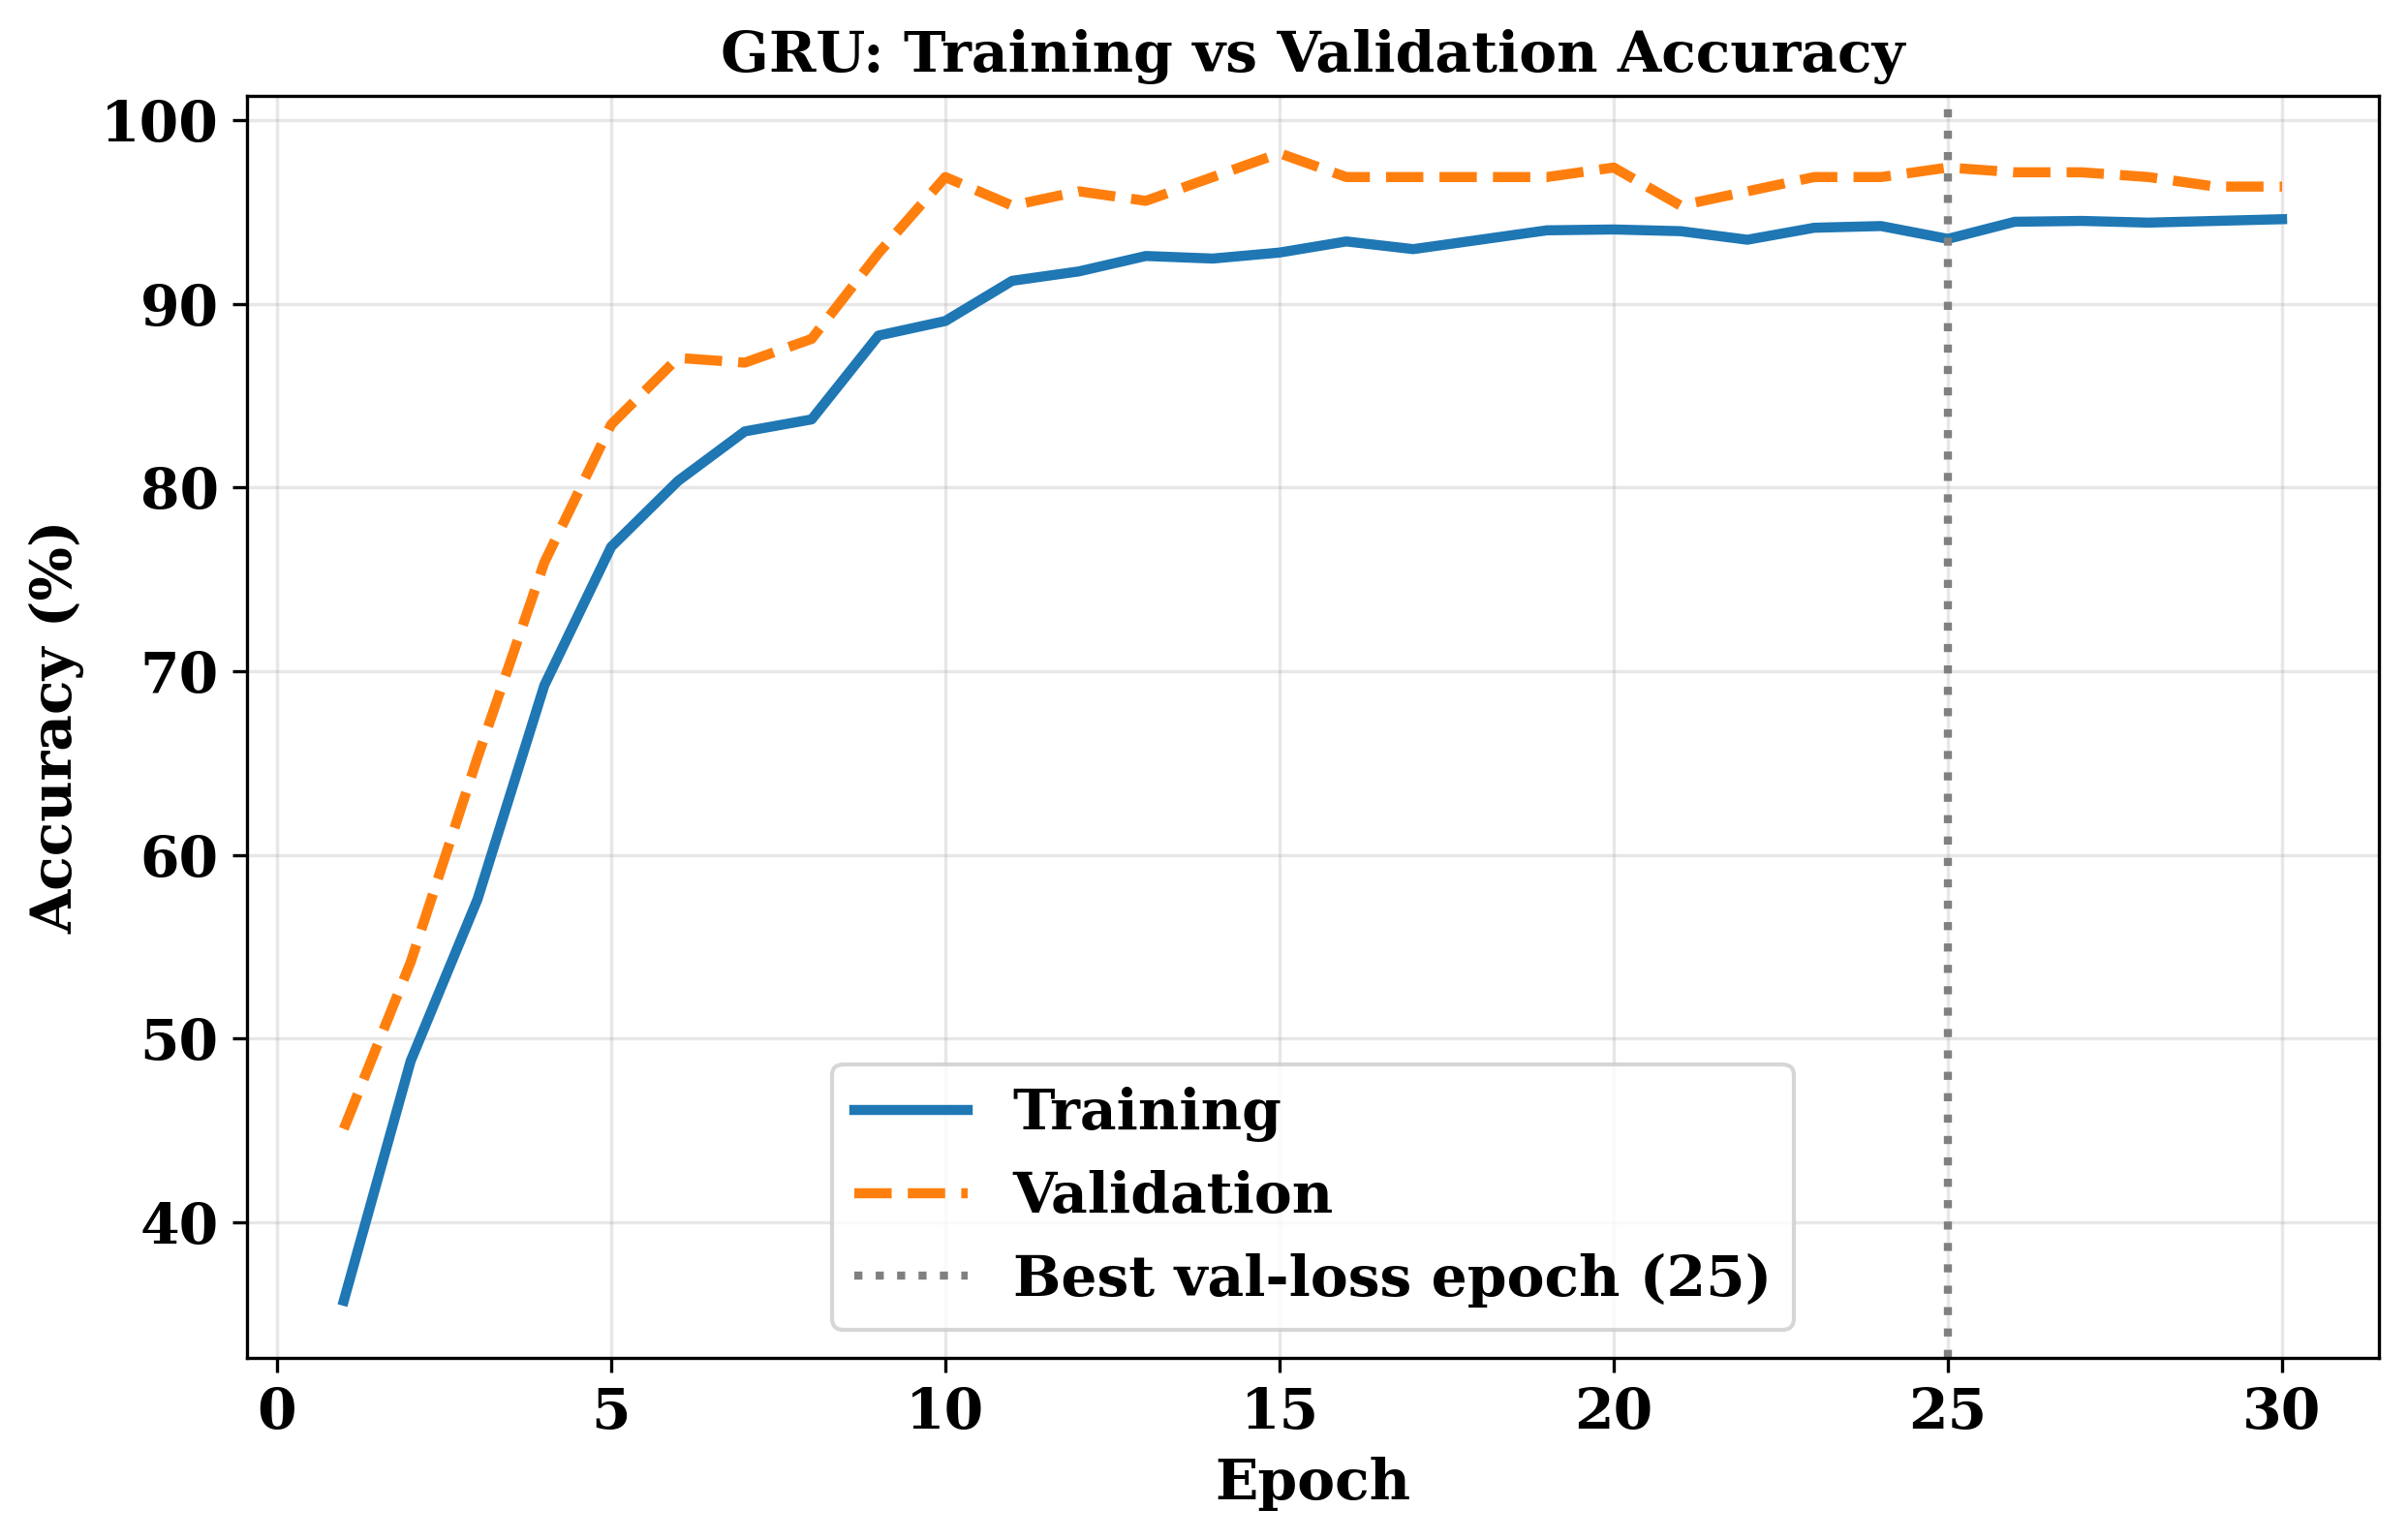
\includegraphics[width=0.48\textwidth]{plot03_accuracy_GRU.png}
\caption{GRU -- Plot 2 (training/validation loss) and Plot 3 (training/validation accuracy).}
\end{figure}

\textbf{Inference (loss):} GRU: train loss $1.62\rightarrow0.13$; val loss
minimum $0.09$ at epoch 25/30, within 5\% of it from epoch 25. Converged,
small generalisation gap -- the update gate gives a short gradient path.

\textbf{Inference (accuracy):} GRU: final train/val accuracy $94.6\%/96.4\%$
(best val $98.2\%$); gap $-1.8$ pts. Train and val track each other
$\rightarrow$ generalises to unseen data.

%%%%%%%%%%%%%%%%%%%%%%%%%%%%%%%%%%%%%%%%%%%%%%%%%%%%%%%%%%%%
\section*{14. Performance Evaluation}

Evaluate each model on the independent test set.

The following metrics are mandatory:

\begin{itemize}
\item Accuracy
\item Precision
\item Recall
\item F1-score
\item Confusion matrix
\item Number of trainable parameters
\item Training time
\end{itemize}

For multi-class classification, report macro-averaged Precision, Recall and
F1-score.

\begin{center}
\begin{tabular}{|l|c|c|c|}
\hline
Metric & RNN & LSTM & GRU\\
\hline
Accuracy (\%) & 72.16 & 94.86 & 98.29\\
Macro Precision (\%) & 72.80 & 95.45 & 98.42\\
Macro Recall (\%) & 74.42 & 94.93 & 98.23\\
Macro F1 (\%) & 73.03 & 94.84 & 98.29\\
Parameters & 1,974 & 6,006 & 4,758\\
Training Time (s) & 30.6 & 25.5 & 26.3\\
\hline
\end{tabular}
\end{center}

\textbf{Inference:} Test macro-F1: GRU $98.3\%>$ LSTM $94.8\%>$ RNN
$73.0\%$. GRU is best ($+25.3$ pts over RNN); gaps under $\sim$1--2 pts may
be noise on 467 test windows.

%%%%%%%%%%%%%%%%%%%%%%%%%%%%%%%%%%%%%%%%%%%%%%%%%%%%%%%%%%%%
\section*{15. Confusion Matrix Analysis}

\begin{figure}[H]
\centering
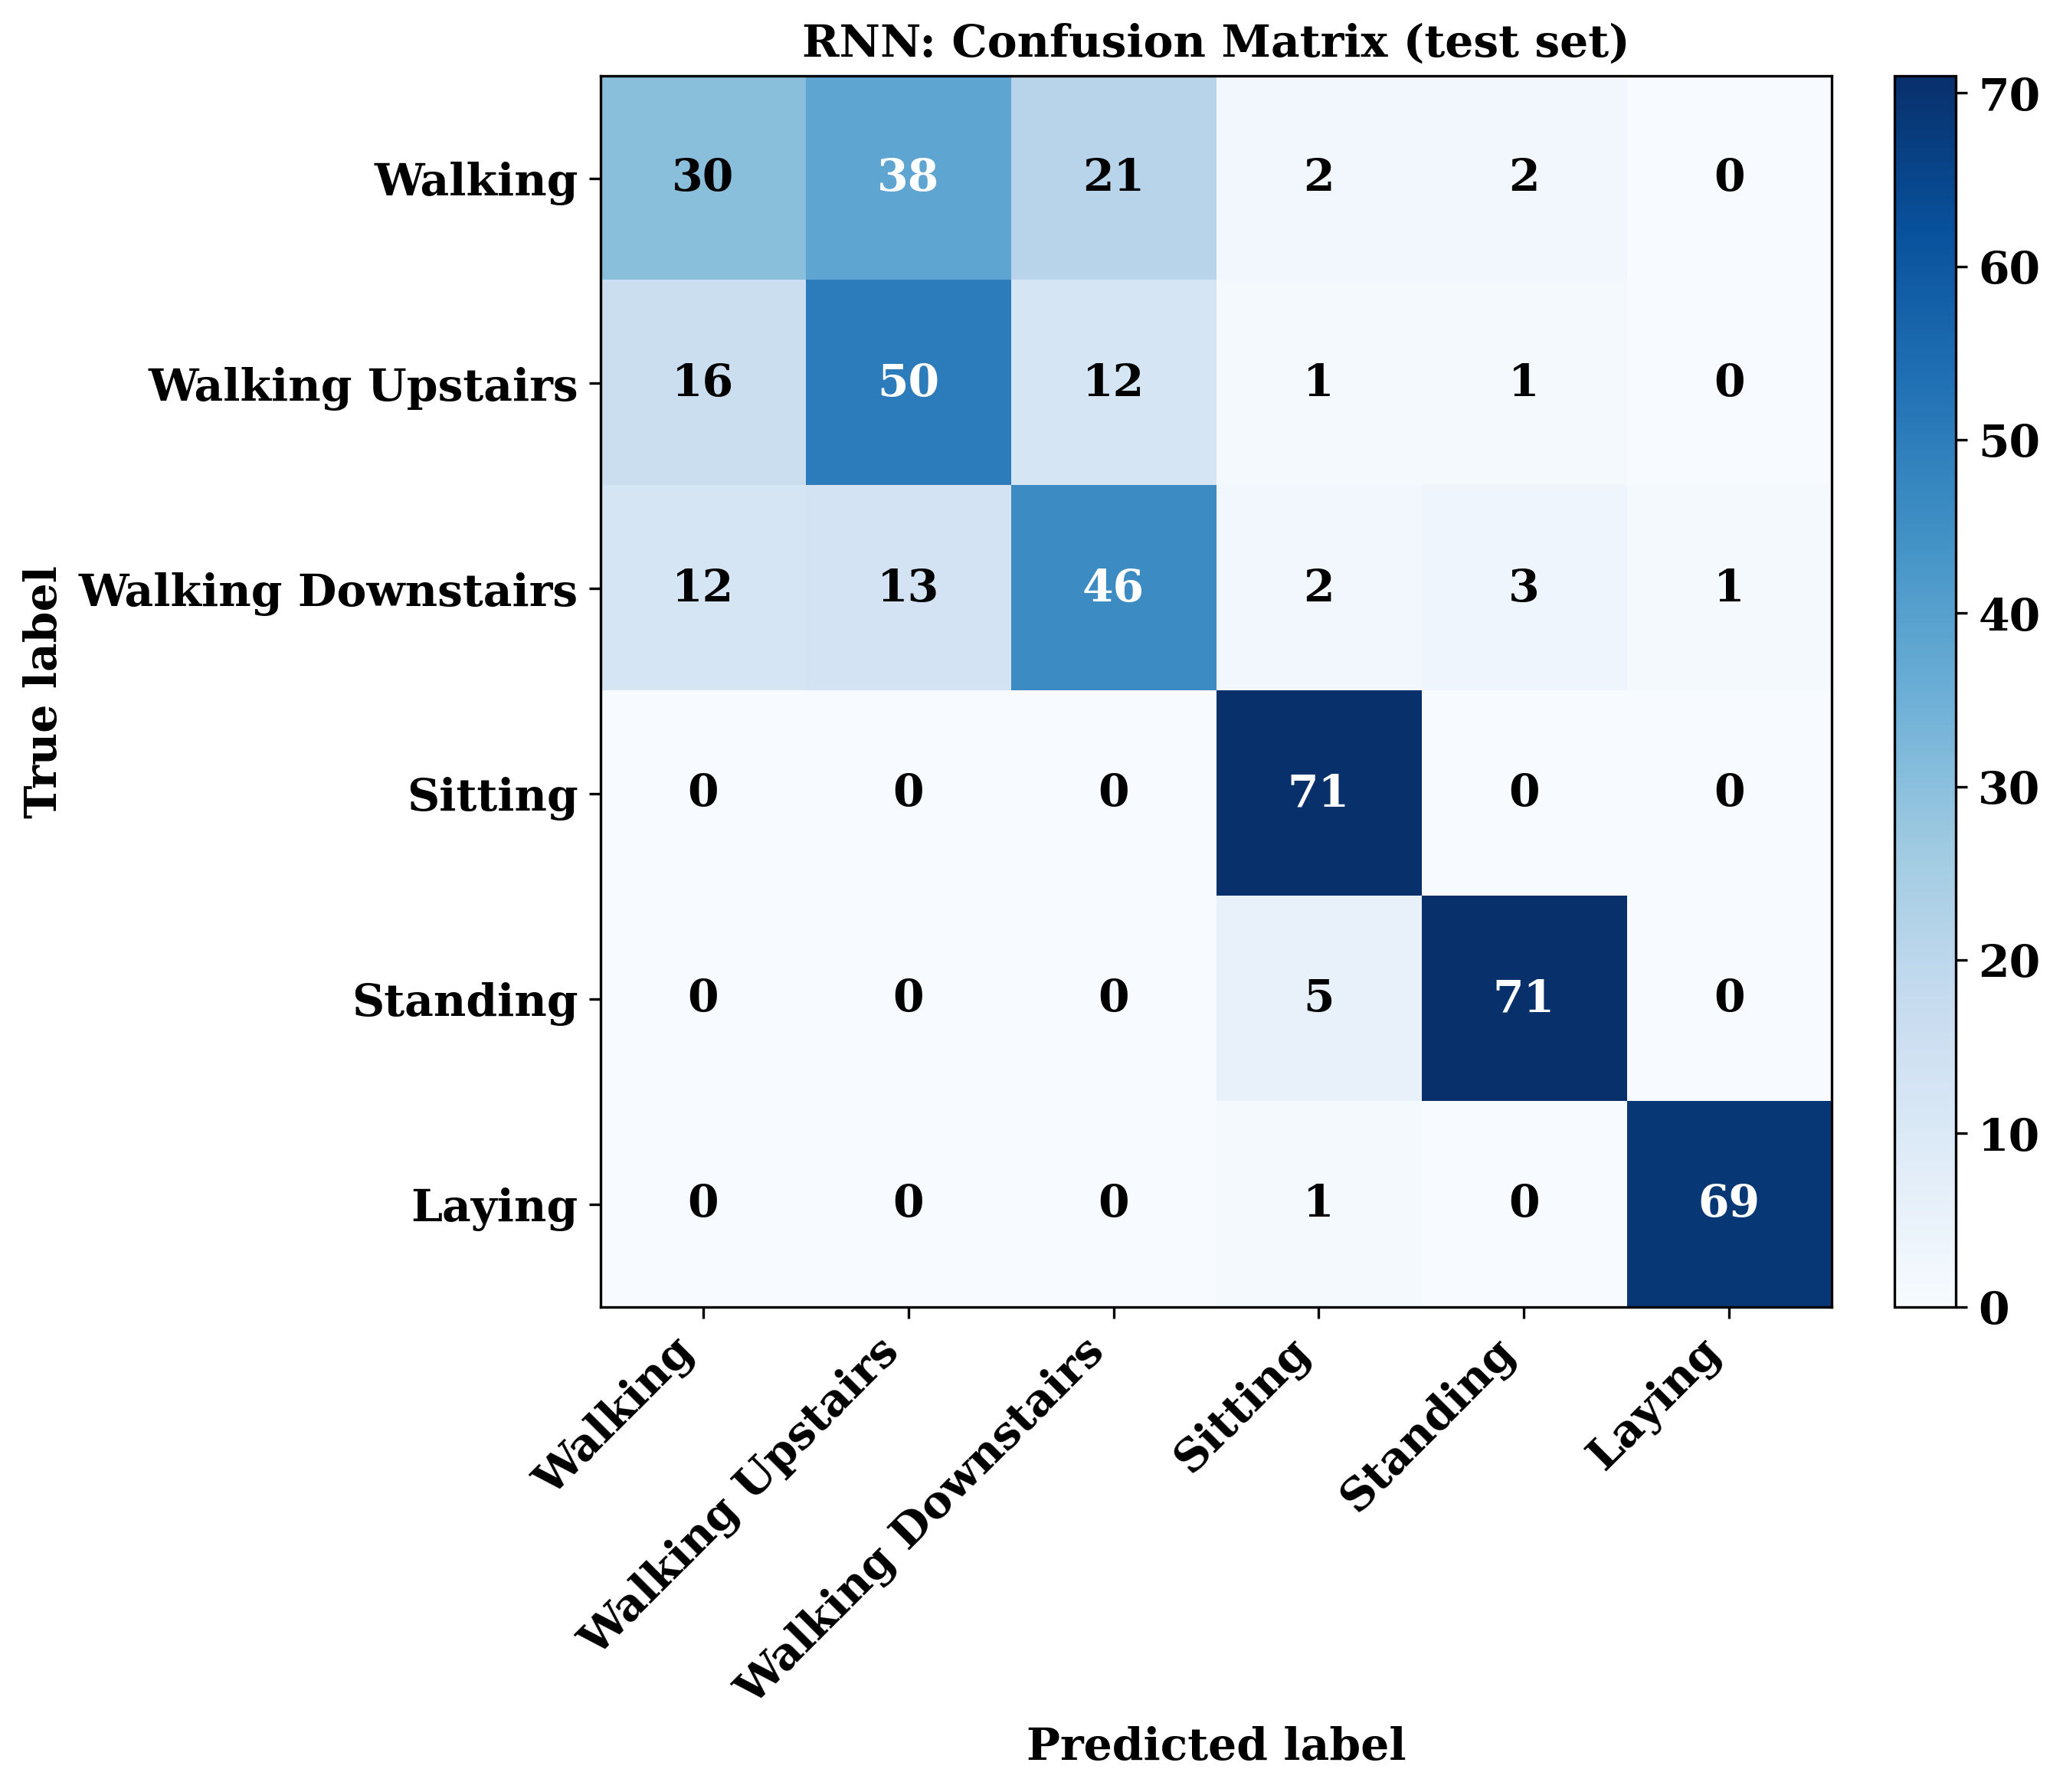
\includegraphics[width=0.6\textwidth]{plot04_confusion_RNN.png}
\caption{Plot 4: RNN confusion matrix (test set).}
\end{figure}

\textbf{Inference:} RNN: best class Sitting (100\%); most errors on Walking
(63 errors, recall 32\%). Top confusion: Walking $\leftrightarrow$ Walking
Upstairs (54 samples) -- similar gait cycles.

\begin{figure}[H]
\centering
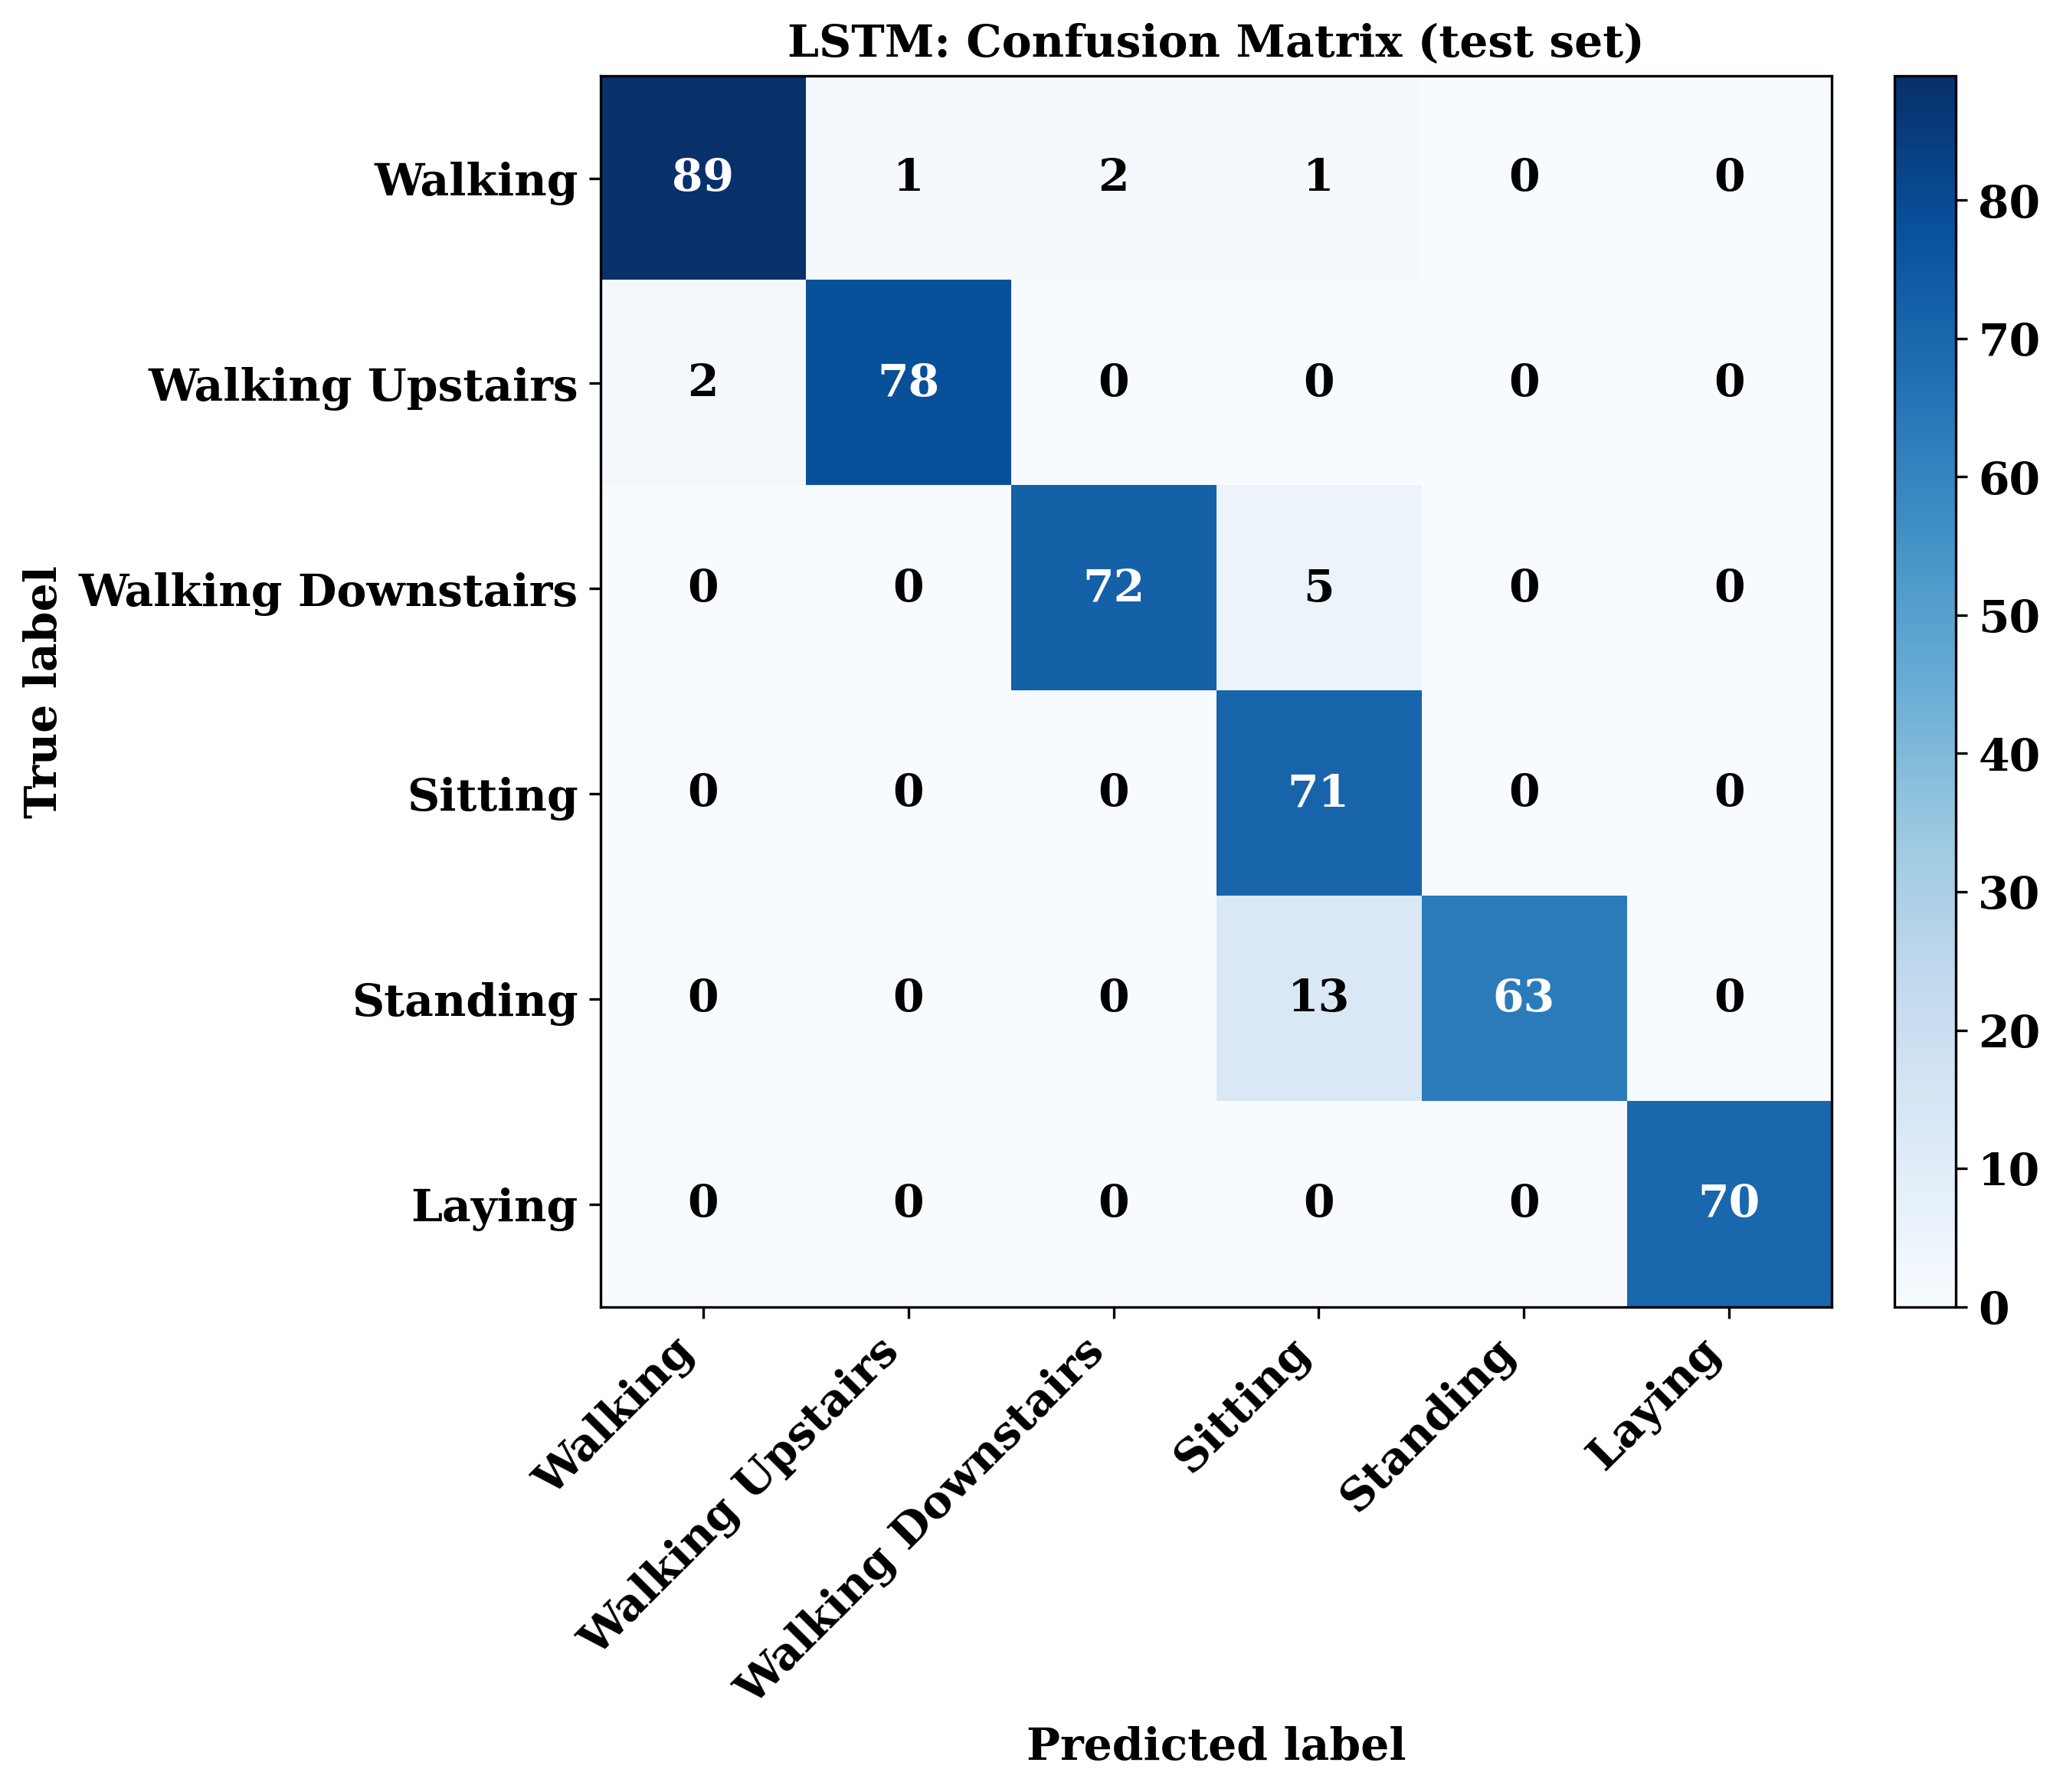
\includegraphics[width=0.6\textwidth]{plot04_confusion_LSTM.png}
\caption{Plot 4: LSTM confusion matrix (test set).}
\end{figure}

\textbf{Inference:} LSTM: best class Sitting (100\%); most errors on
Standing (13 errors, recall 83\%). Top confusion: Sitting $\leftrightarrow$
Standing (13 samples) -- both near-static postures.

\begin{figure}[H]
\centering
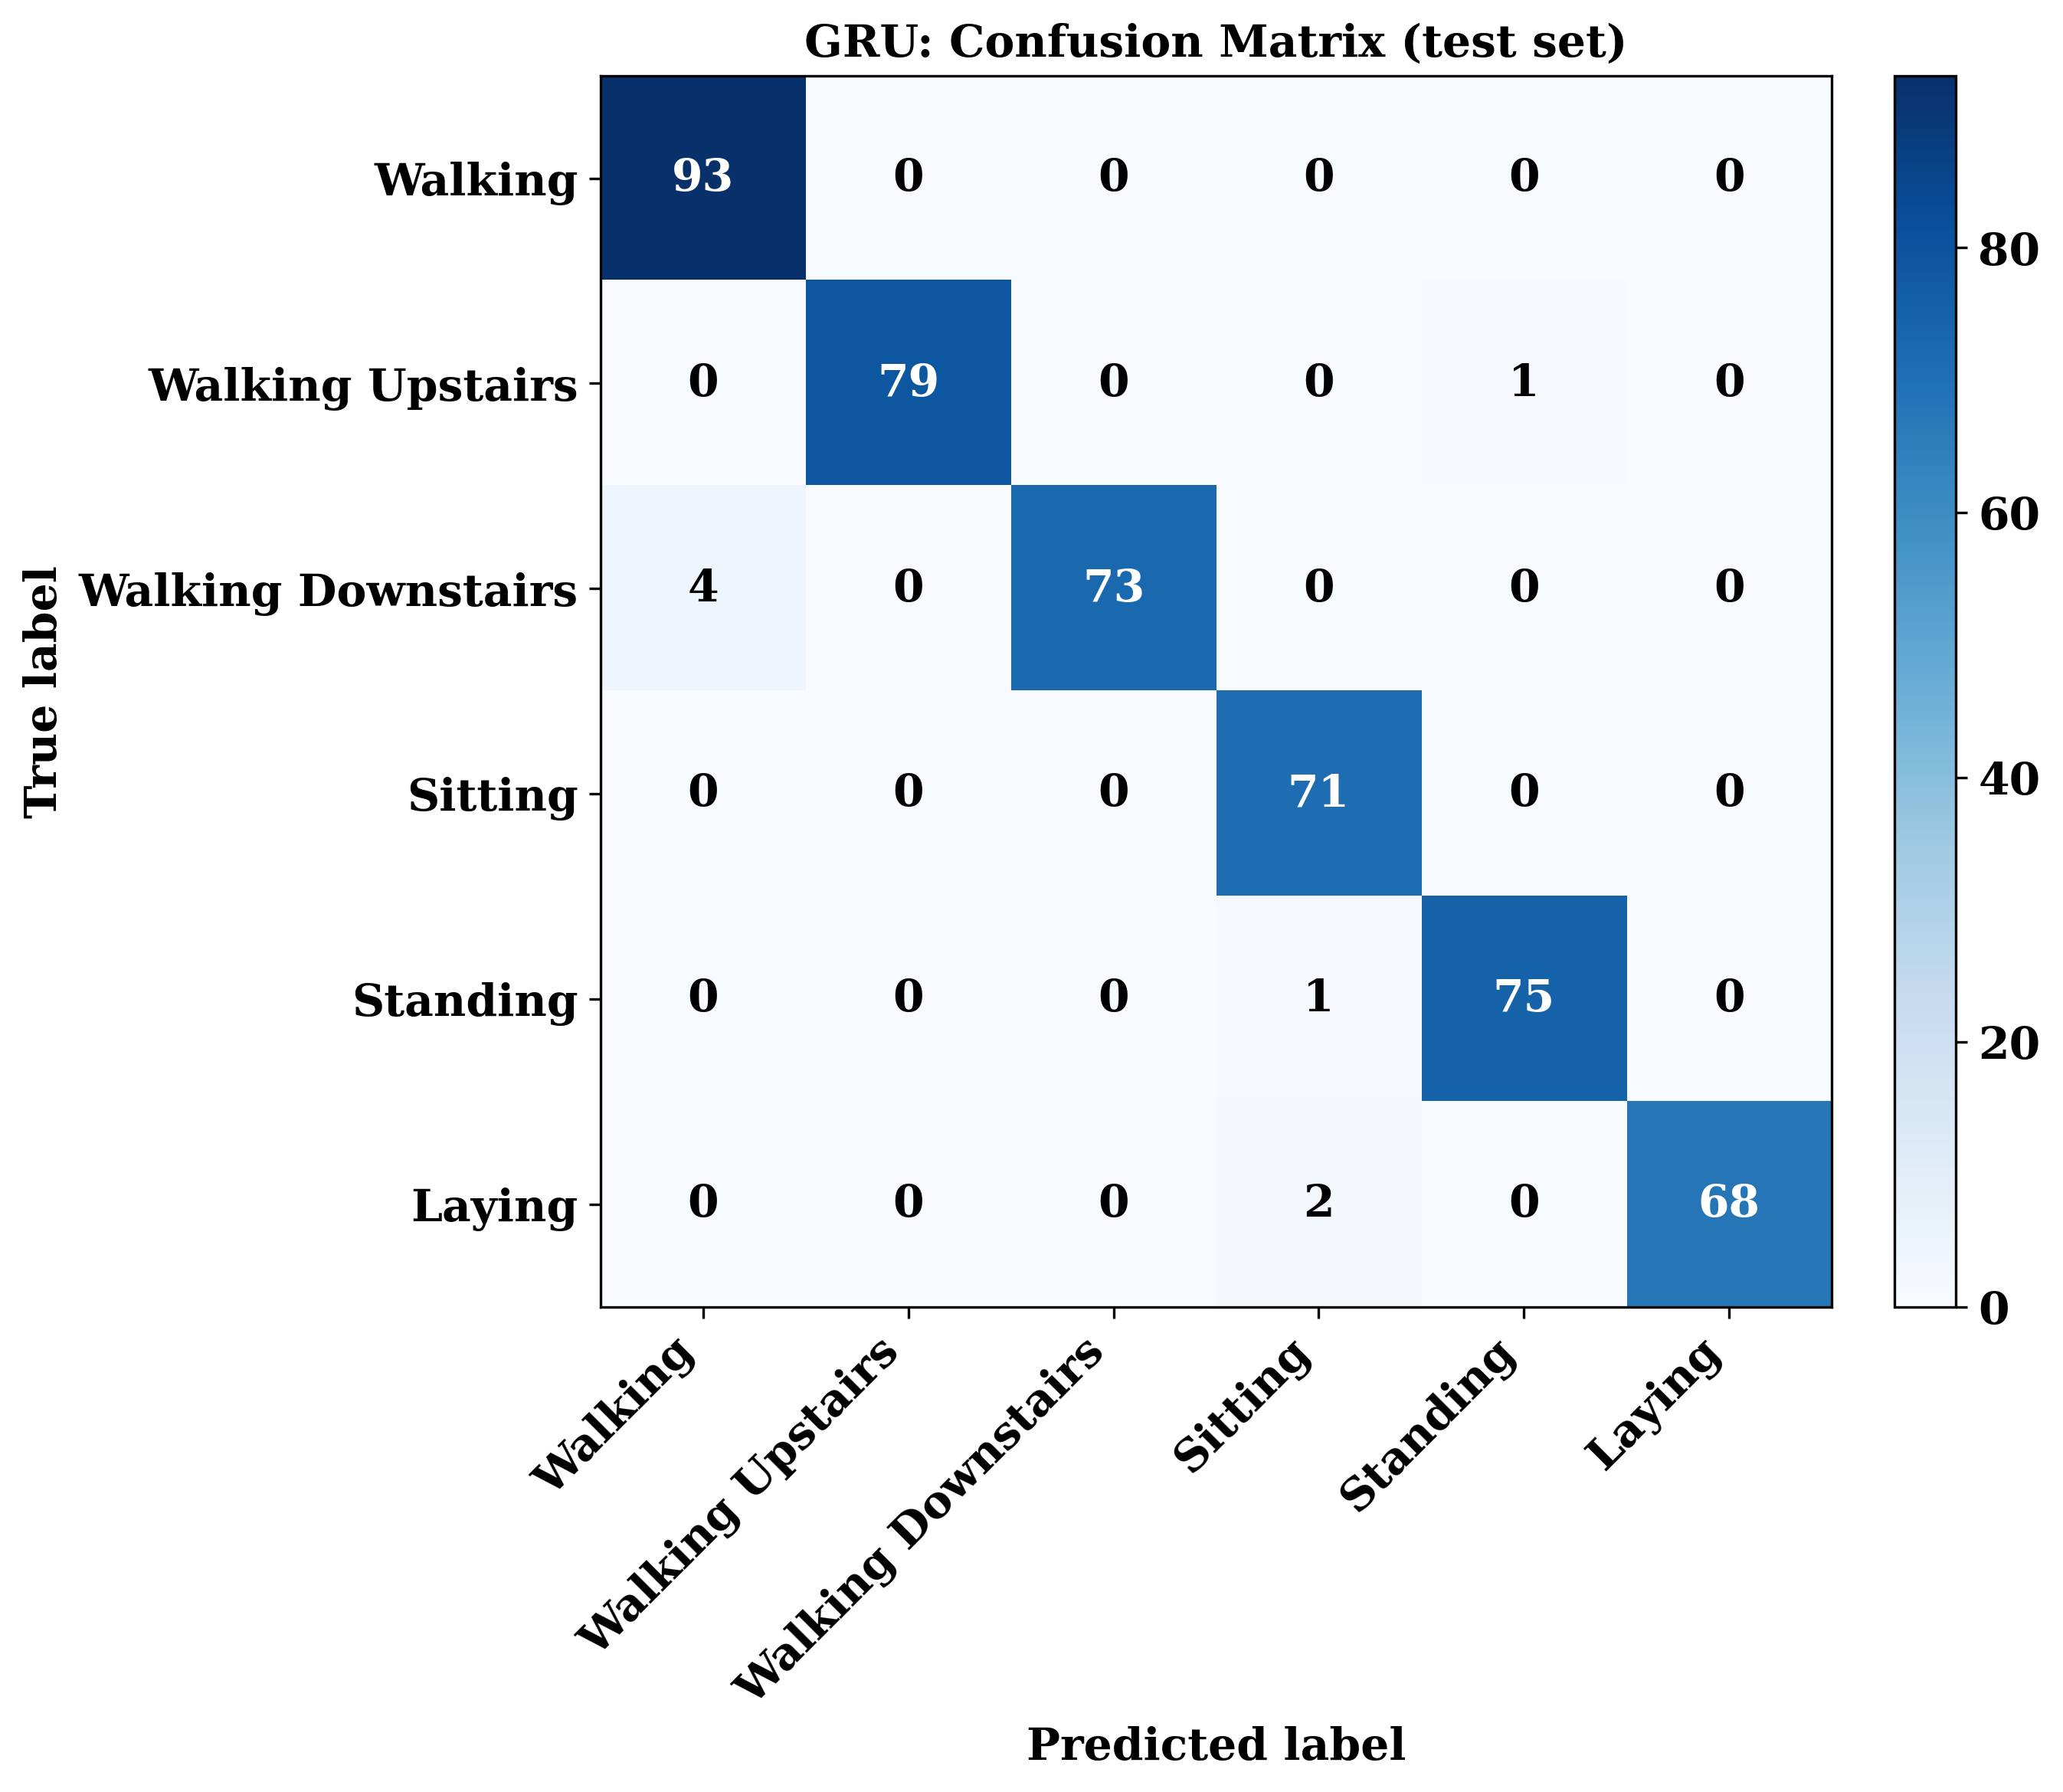
\includegraphics[width=0.6\textwidth]{plot04_confusion_GRU.png}
\caption{Plot 4: GRU confusion matrix (test set).}
\end{figure}

\textbf{Inference:} GRU: best class Walking (100\%); most errors on Walking
Downstairs (4 errors, recall 95\%). Top confusion: Walking $\leftrightarrow$
Walking Downstairs (4 samples) -- similar gait cycles.

\textbf{Consistency across models:} Most-errors class -- RNN = Walking,
LSTM = Standing, GRU = Walking Downstairs. The top confusion pair is
different across models, so errors are \emph{model-specific} rather than
uniformly shared by RNN, LSTM and GRU.

%%%%%%%%%%%%%%%%%%%%%%%%%%%%%%%%%%%%%%%%%%%%%%%%%%%%%%%%%%%%
\section*{16. RNN vs. LSTM vs. GRU Comparison}

Students must complete the following table.

\begin{center}
\begin{tabular}{|l|c|c|c|}
\hline
Property & RNN & LSTM & GRU\\
\hline
Hidden state & Yes & Yes & Yes\\
Cell state & No & Yes & No\\
Forget gate & No & Yes & No\\
Input gate & No & Yes & No\\
Output gate & No & Yes & No\\
Update gate & No & No & Yes\\
Reset gate & No & No & Yes\\
Parameters & 1,974 & 6,006 & 4,758\\
Training time & 30.6 s & 25.5 s & 26.3 s\\
Test F1-score & 73.03\% & 94.84\% & 98.29\%\\
\hline
\end{tabular}
\end{center}

\textbf{Model Performance Comparison}

\begin{figure}[H]
\centering
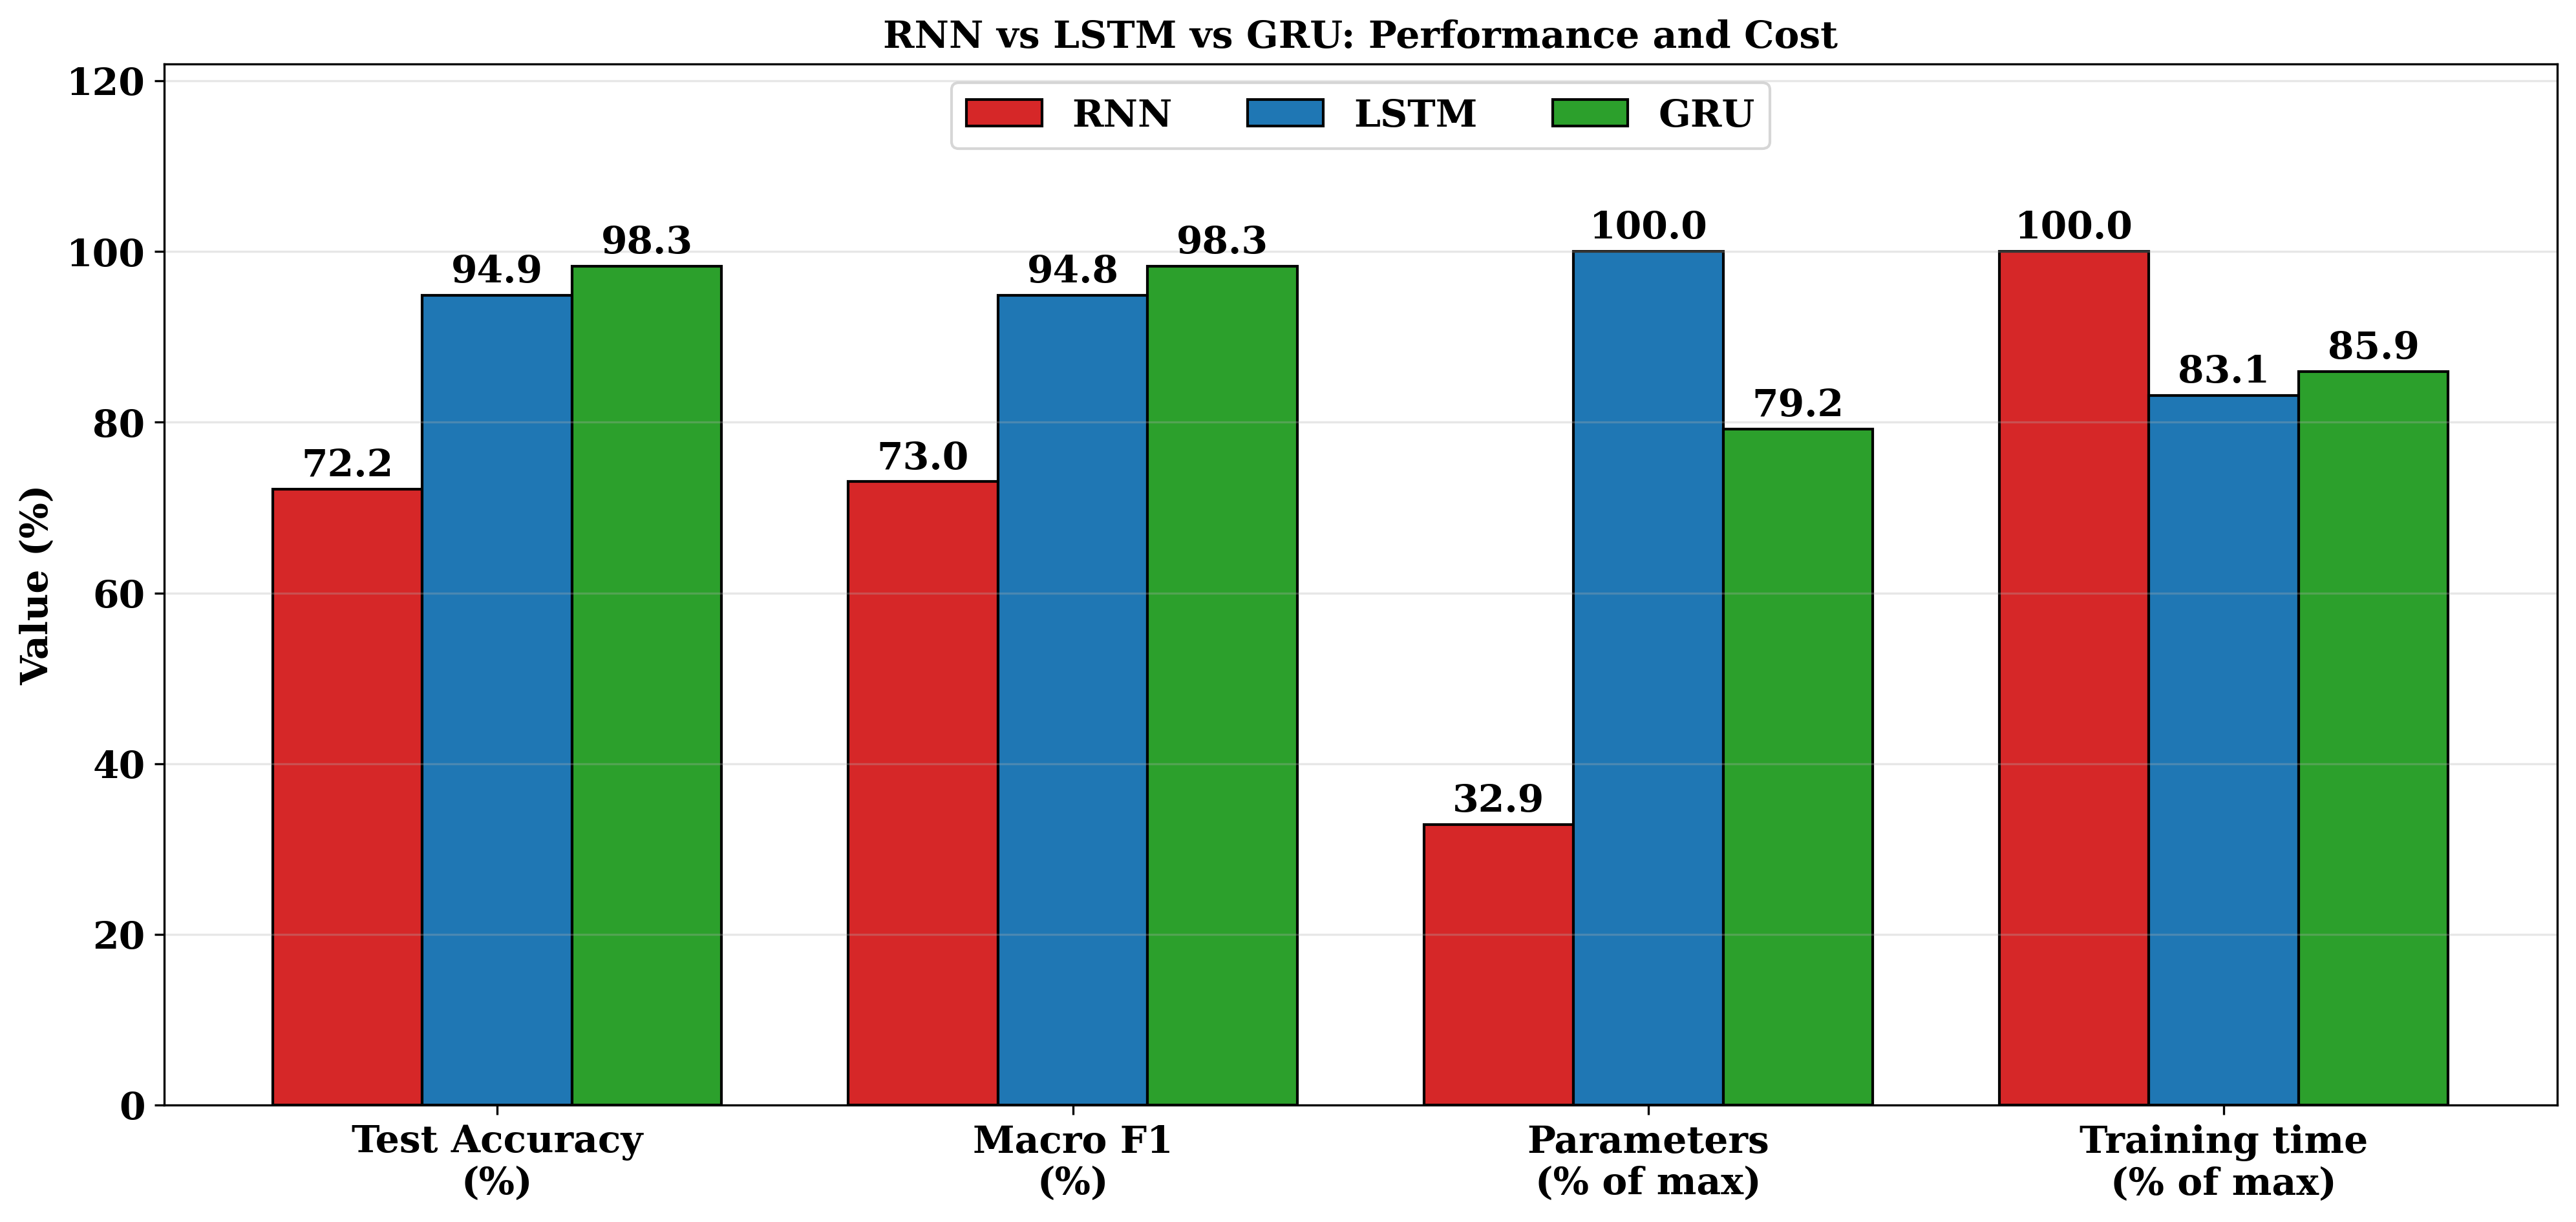
\includegraphics[width=0.85\textwidth]{plot05_model_comparison.png}
\caption{Plot 5: Test accuracy, macro F1, parameters and training time (normalised to the maximum across models).}
\end{figure}

\textbf{Inference:} F1 -- RNN 73.0, LSTM 94.8, GRU 98.3; parameter ratio
$1{:}3.0{:}2.4$; time ratio $1{:}0.8{:}0.9$ (RNN:LSTM:GRU). Trade-off: GRU
has the best F1; GRU vs LSTM is $+3.5$ F1 pts with 21\% fewer parameters and
3\% more training time -- here GRU dominates LSTM on both accuracy and
compactness for this dataset.

%%%%%%%%%%%%%%%%%%%%%%%%%%%%%%%%%%%%%%%%%%%%%%%%%%%%%%%%%%%%
\section*{17. Effect of Sequence Length}

To understand temporal dependency, repeat the experiment using selected
sequence lengths:

\[
T\in\{32,64,128\}.
\]

When reducing the sequence length, truncate or construct the input consistently.

\begin{center}
\begin{tabular}{|c|c|c|c|}
\hline
Sequence Length & RNN F1 (\%) & LSTM F1 (\%) & GRU F1 (\%)\\
\hline
32 & 81.97 & 87.91 & 94.08\\
64 & 82.01 & 93.22 & 97.55\\
128 & 73.03 & 94.84 & 98.29\\
\hline
\end{tabular}
\end{center}

\textbf{Sequence Length vs. Test F1-score}

\begin{center}
\begin{tabular}{|c|c|c|c|}
\hline
Sequence Length & RNN time (s) & LSTM time (s) & GRU time (s)\\
\hline
32 & 20.5 & 21.6 & 19.6\\
64 & 21.8 & 21.3 & 21.0\\
128 & 30.6 & 25.5 & 26.3\\
\hline
\end{tabular}
\end{center}

\begin{figure}[H]
\centering
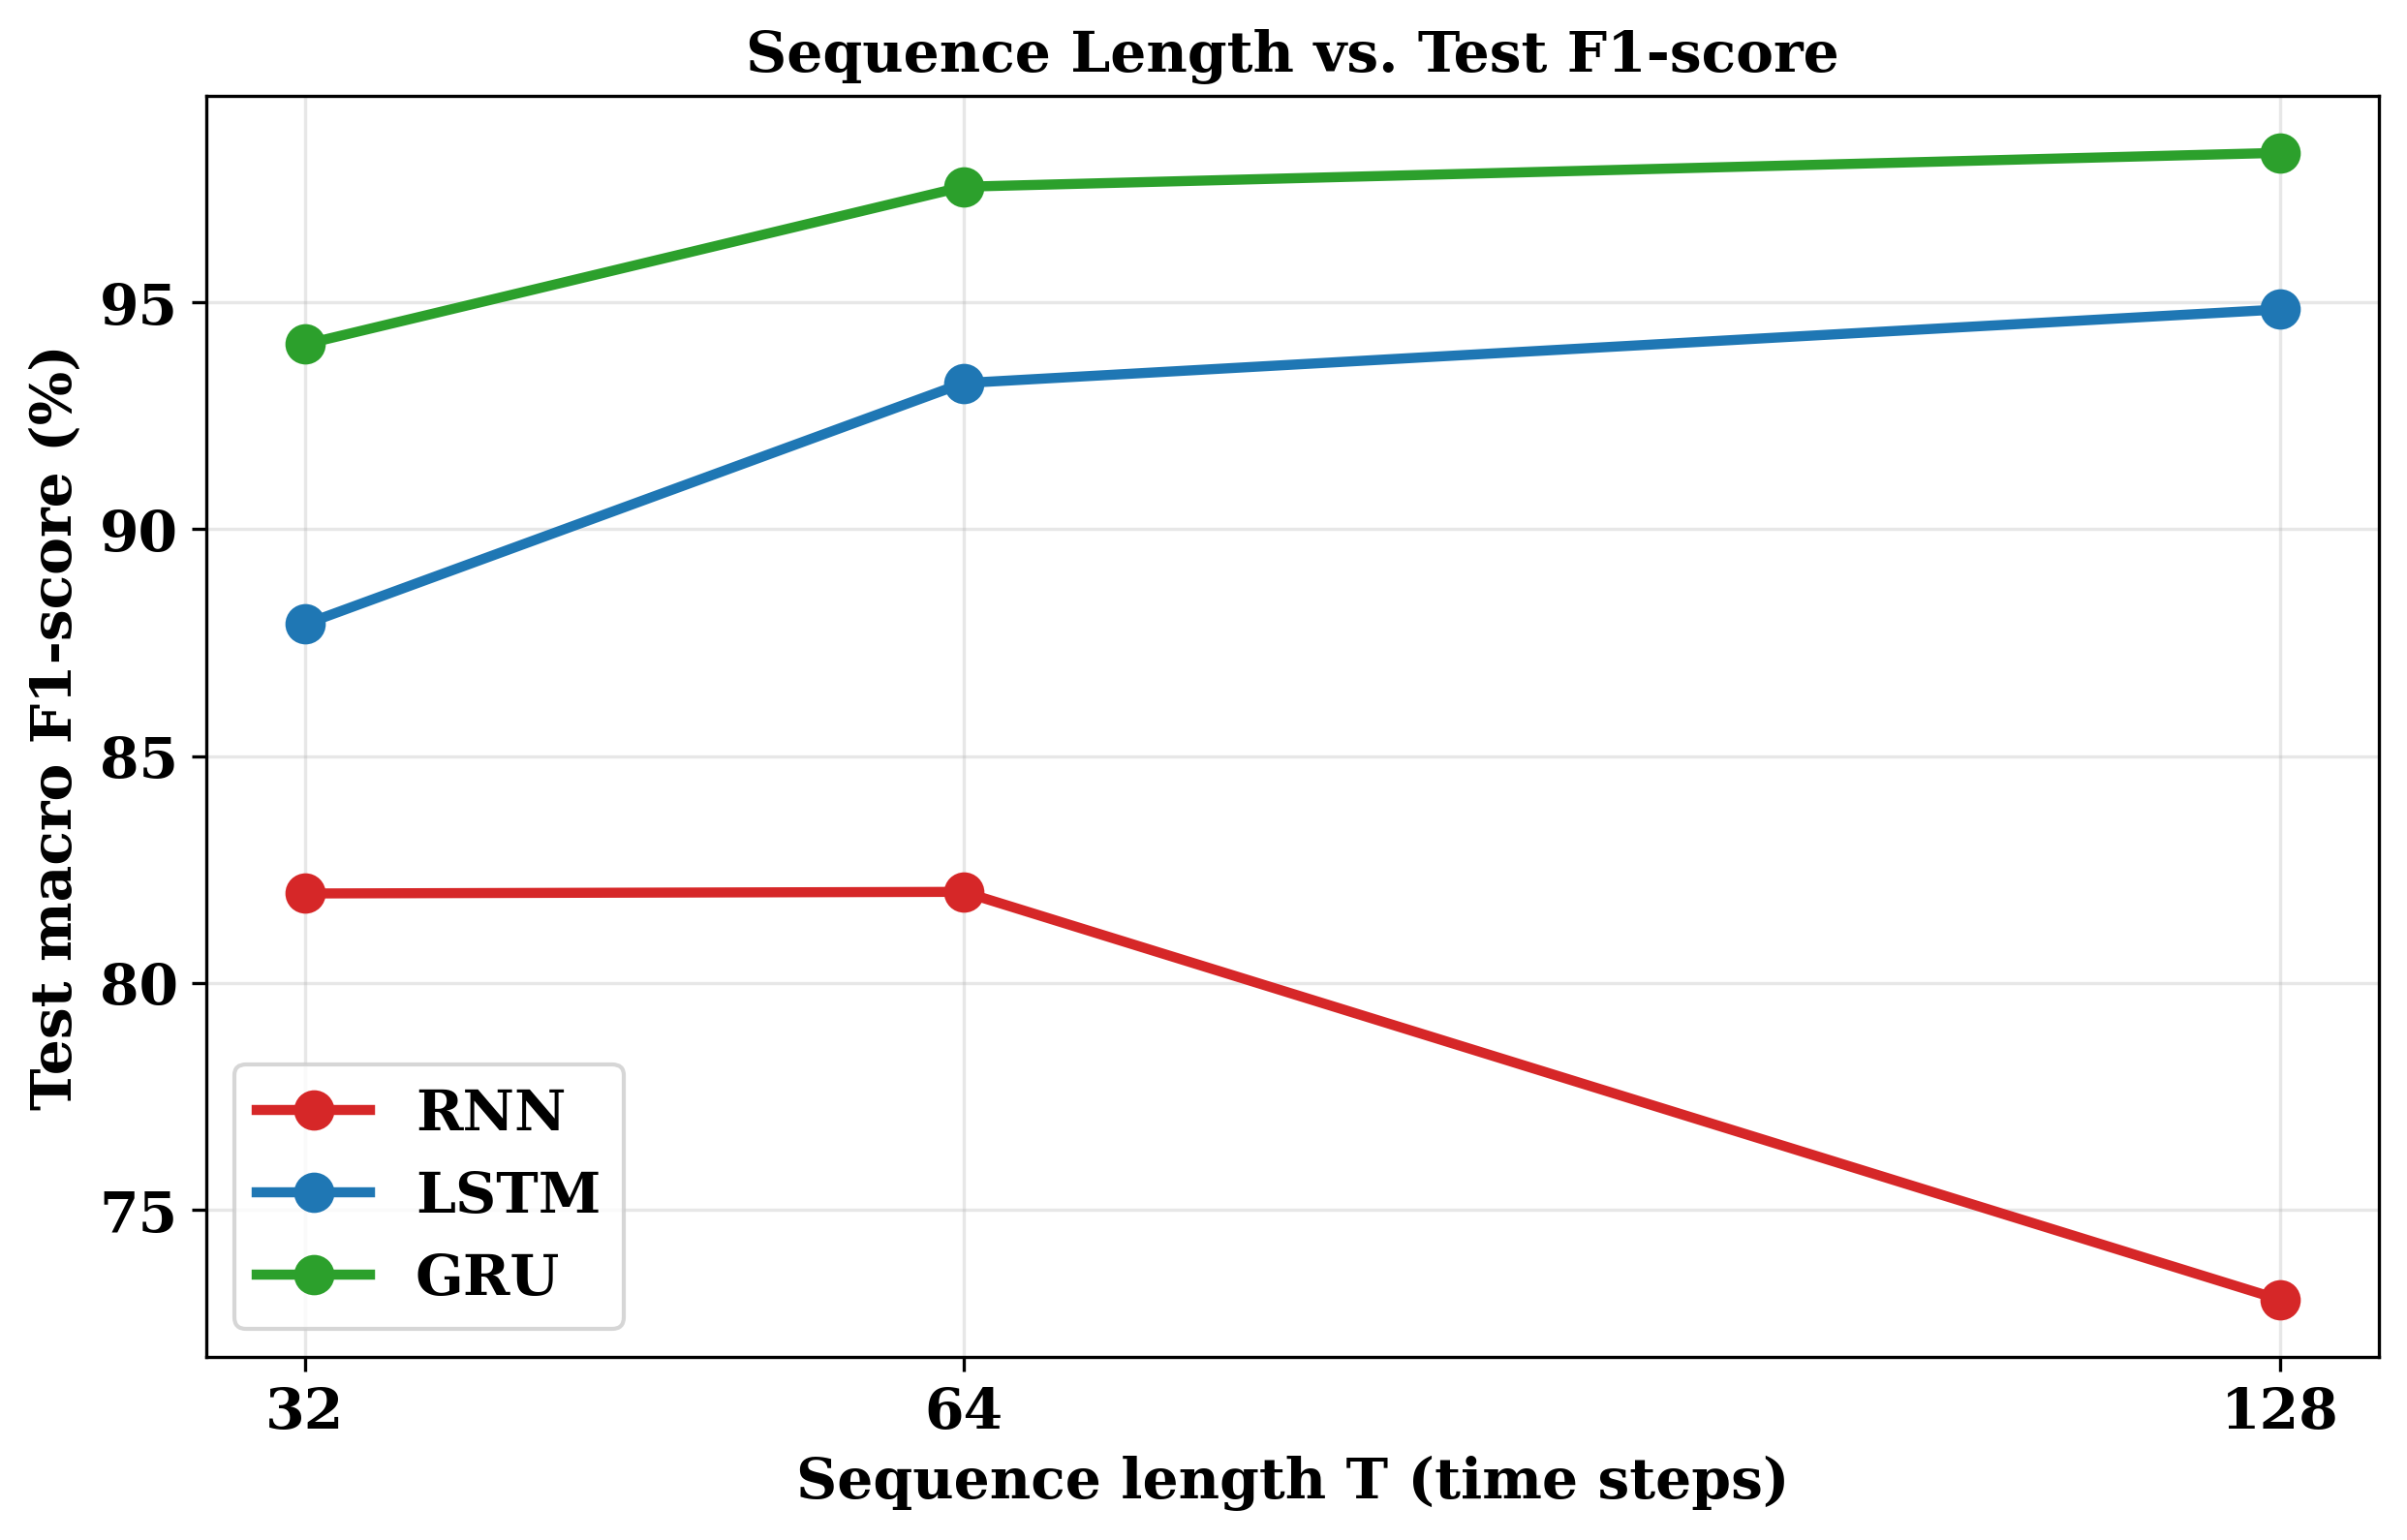
\includegraphics[width=0.7\textwidth]{plot06_sequence_length_vs_f1.png}
\caption{Plot 6: Test macro F1-score versus sequence length $T\in\{32,64,128\}$.}
\end{figure}

\textbf{Inference:} Test F1, $T=32\rightarrow128$: RNN $82.0\rightarrow73.0$,
LSTM $87.9\rightarrow94.8$, GRU $94.1\rightarrow98.3$. LSTM and GRU improve
with more temporal context, while RNN's F1 falls with longer sequences
(largest change: RNN, $-8.9$ pts) -- consistent with vanishing gradients
making a 128-step plain RNN harder to train than a 32-step one, whereas the
gated models exploit the extra context.

%%%%%%%%%%%%%%%%%%%%%%%%%%%%%%%%%%%%%%%%%%%%%%%%%%%%%%%%%%%%
\section*{18. Video Understanding Using CNN and RNN}

This part demonstrates the application:

\[
\boxed{\text{Video Understanding using CNN + RNN}}
\]

A video is a sequence of image frames. CNNs are used to extract spatial
features from individual frames, while RNN/LSTM/GRU models the temporal
relationship among those features.

The complete pipeline is:

\begin{center}
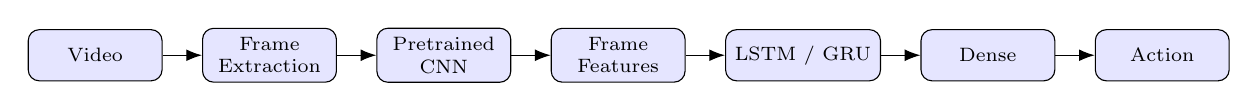
\begin{tikzpicture}[node distance=5mm]
\node[layer](a){Video};
\node[layer,right=of a](b){Frame\\Extraction};
\node[layer,right=of b](c){Pretrained\\CNN};
\node[layer,right=of c](d){Frame\\Features};
\node[layer,right=of d](e){LSTM / GRU};
\node[layer,right=of e](f){Dense};
\node[layer,right=of f](g){Action};

\foreach \x/\y in {a/b,b/c,c/d,d/e,e/f,f/g}
\draw[arrow](\x)--(\y);
\end{tikzpicture}
\end{center}

\subsection*{Recommended Dataset}

Use a small subset of the UCF101 action-recognition dataset:

\url{https://www.crcv.ucf.edu/data/UCF101.php}

Select only 3--5 action classes and a small number of videos per class so that
the experiment remains computationally manageable.

Possible classes include:

\begin{itemize}
\item Basketball
\item Biking
\item Walking
\item Running
\item TennisSwing
\end{itemize}

The objective is to understand the CNN--recurrent pipeline rather than to
train a state-of-the-art video recognition system.

\subsection*{Observed Results}

A small UCF101 subset (\texttt{sayakpaul/ucf101-subset} on the Hugging Face
hub) was used. Of the manual's suggested classes only \emph{Basketball} was
available in this subset, so the remaining four classes were automatically
filled with the largest available UCF101 categories:

\begin{verbatim}
Selected action classes: ['Basketball', 'BaseballPitch', 'BabyCrawling',
                           'BenchPress', 'BandMarching']
Videos per class: {'Basketball': 44, 'BaseballPitch': 43, 'BabyCrawling': 42,
                    'BenchPress': 42, 'BandMarching': 42}
\end{verbatim}

40 videos per class were used (200 videos total).

%%%%%%%%%%%%%%%%%%%%%%%%%%%%%%%%%%%%%%%%%%%%%%%%%%%%%%%%%%%%
\section*{19. Expected Video Input and Output}

Sample 10 frames uniformly from each video.

Each frame is resized to

\[
224\times224\times3.
\]

A pretrained CNN such as MobileNetV2 is used only as a feature extractor.

If the CNN produces a feature vector of dimension $D$, then the recurrent
network receives:

\[
X\in\mathbb{R}^{10\times D}.
\]

For a batch of $B$ videos:

\[
X\in\mathbb{R}^{B\times10\times D}.
\]

The expected output is a probability vector over the selected action classes.

For example:

\begin{verbatim}
Predicted class : Basketball
Actual class    : Basketball
Confidence      : 0.xx
\end{verbatim}

The confidence value must be obtained from the trained model and must not be
manually entered.

\subsection*{Observed Results}

Frame tensor per video: $(10,224,224,3)$; CNN feature dimension
$D=1280$ (MobileNetV2 global-average-pooled output); feature tensor supplied
to the recurrent network: $(200,10,1280)$, i.e.\ $(B,10,D)$.

\begin{verbatim}
Model: CNN-GRU (selected recurrent architecture, see Section 21)

Video: v_Basketball_g01_c03.avi
   Predicted class : Basketball
   Actual class    : Basketball
   Confidence      : 0.99

Video: v_Basketball_g01_c05.avi
   Predicted class : Basketball
   Actual class    : Basketball
   Confidence      : 0.99

Video: v_Basketball_g17_c04.avi
   Predicted class : Basketball
   Actual class    : Basketball
   Confidence      : 1.00

Video: v_Basketball_g24_c04.avi
   Predicted class : Basketball
   Actual class    : Basketball
   Confidence      : 1.00
\end{verbatim}

All confidence values above were read directly from the trained model's
softmax output.

%%%%%%%%%%%%%%%%%%%%%%%%%%%%%%%%%%%%%%%%%%%%%%%%%%%%%%%%%%%%
\section*{20. CNN Feature Extraction}

Use a pretrained CNN with the classification head removed.

\begin{center}
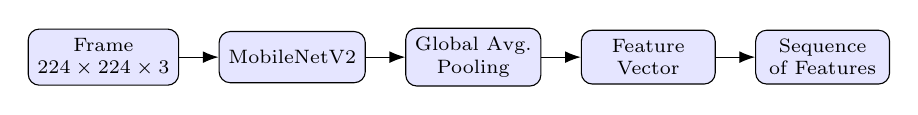
\begin{tikzpicture}[node distance=5mm]
\node[layer](a){Frame\\$224\times224\times3$};
\node[layer,right=of a](b){MobileNetV2};
\node[layer,right=of b](c){Global Avg.\\Pooling};
\node[layer,right=of c](d){Feature\\Vector};
\node[layer,right=of d](e){Sequence\\of Features};

\foreach \x/\y in {a/b,b/c,c/d,d/e}
\draw[arrow](\x)--(\y);
\end{tikzpicture}
\end{center}

Do not train the CNN from scratch. Freeze the pretrained CNN and extract
features first. Then train the recurrent classifier.

\subsection*{Observed Results}

CNN feature dimension: $D=1280$ (MobileNetV2, frozen, ImageNet weights,
\texttt{include\_top=False}, global average pooling). Resulting tensor
supplied to the recurrent network: $(200,10,1280)$, i.e.\ $B=200$ videos,
10 frames per video, 1280 features per frame.

%%%%%%%%%%%%%%%%%%%%%%%%%%%%%%%%%%%%%%%%%%%%%%%%%%%%%%%%%%%%
\section*{21. CNN--LSTM / CNN--GRU Model}

Use the following architecture:

\begin{center}
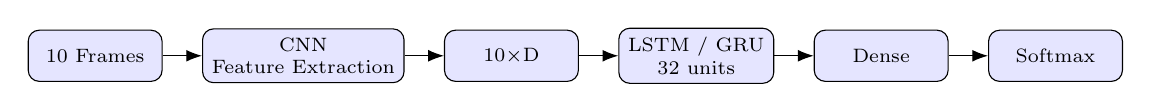
\begin{tikzpicture}[node distance=5mm]
\node[layer](a){10 Frames};
\node[layer,right=of a](b){CNN\\Feature Extraction};
\node[layer,right=of b](c){10$\times$D};
\node[layer,right=of c](d){LSTM / GRU\\32 units};
\node[layer,right=of d](e){Dense};
\node[layer,right=of e](f){Softmax};

\foreach \x/\y in {a/b,b/c,c/d,d/e,e/f}
\draw[arrow](\x)--(\y);
\end{tikzpicture}
\end{center}

\subsection*{Observed Results}

The 200 videos were split group-aware (by UCF101 group id) into
139 training / 28 validation / 33 test videos. Both CNN--LSTM and CNN--GRU
(32 recurrent units) were trained on the identical cached CNN features for
40 epochs:

\begin{verbatim}
CNN-LSTM: epoch 1  | loss 1.3697  acc  46.8% | val_loss 1.2076  val_acc  64.3%
          epoch 10 | loss 0.0790  acc 100.0% | val_loss 0.1334  val_acc 100.0%
          epoch 40 | loss 0.0061  acc 100.0% | val_loss 0.0276  val_acc 100.0%
==> CNN-LSTM: test acc 93.9% | F1 93.8% | parameters 169,285 | val F1 100.0%

CNN-GRU:  epoch 1  | loss 1.4449  acc  40.3% | val_loss 0.9989  val_acc  71.4%
          epoch 10 | loss 0.0538  acc 100.0% | val_loss 0.1135  val_acc 100.0%
          epoch 40 | loss 0.0047  acc 100.0% | val_loss 0.0193  val_acc 100.0%
==> CNN-GRU:  test acc 93.9% | F1 93.8% | parameters 127,365 | val F1 100.0%

Selected recurrent model for the video plots (best validation F1): GRU
\end{verbatim}

\begin{figure}[H]
\centering
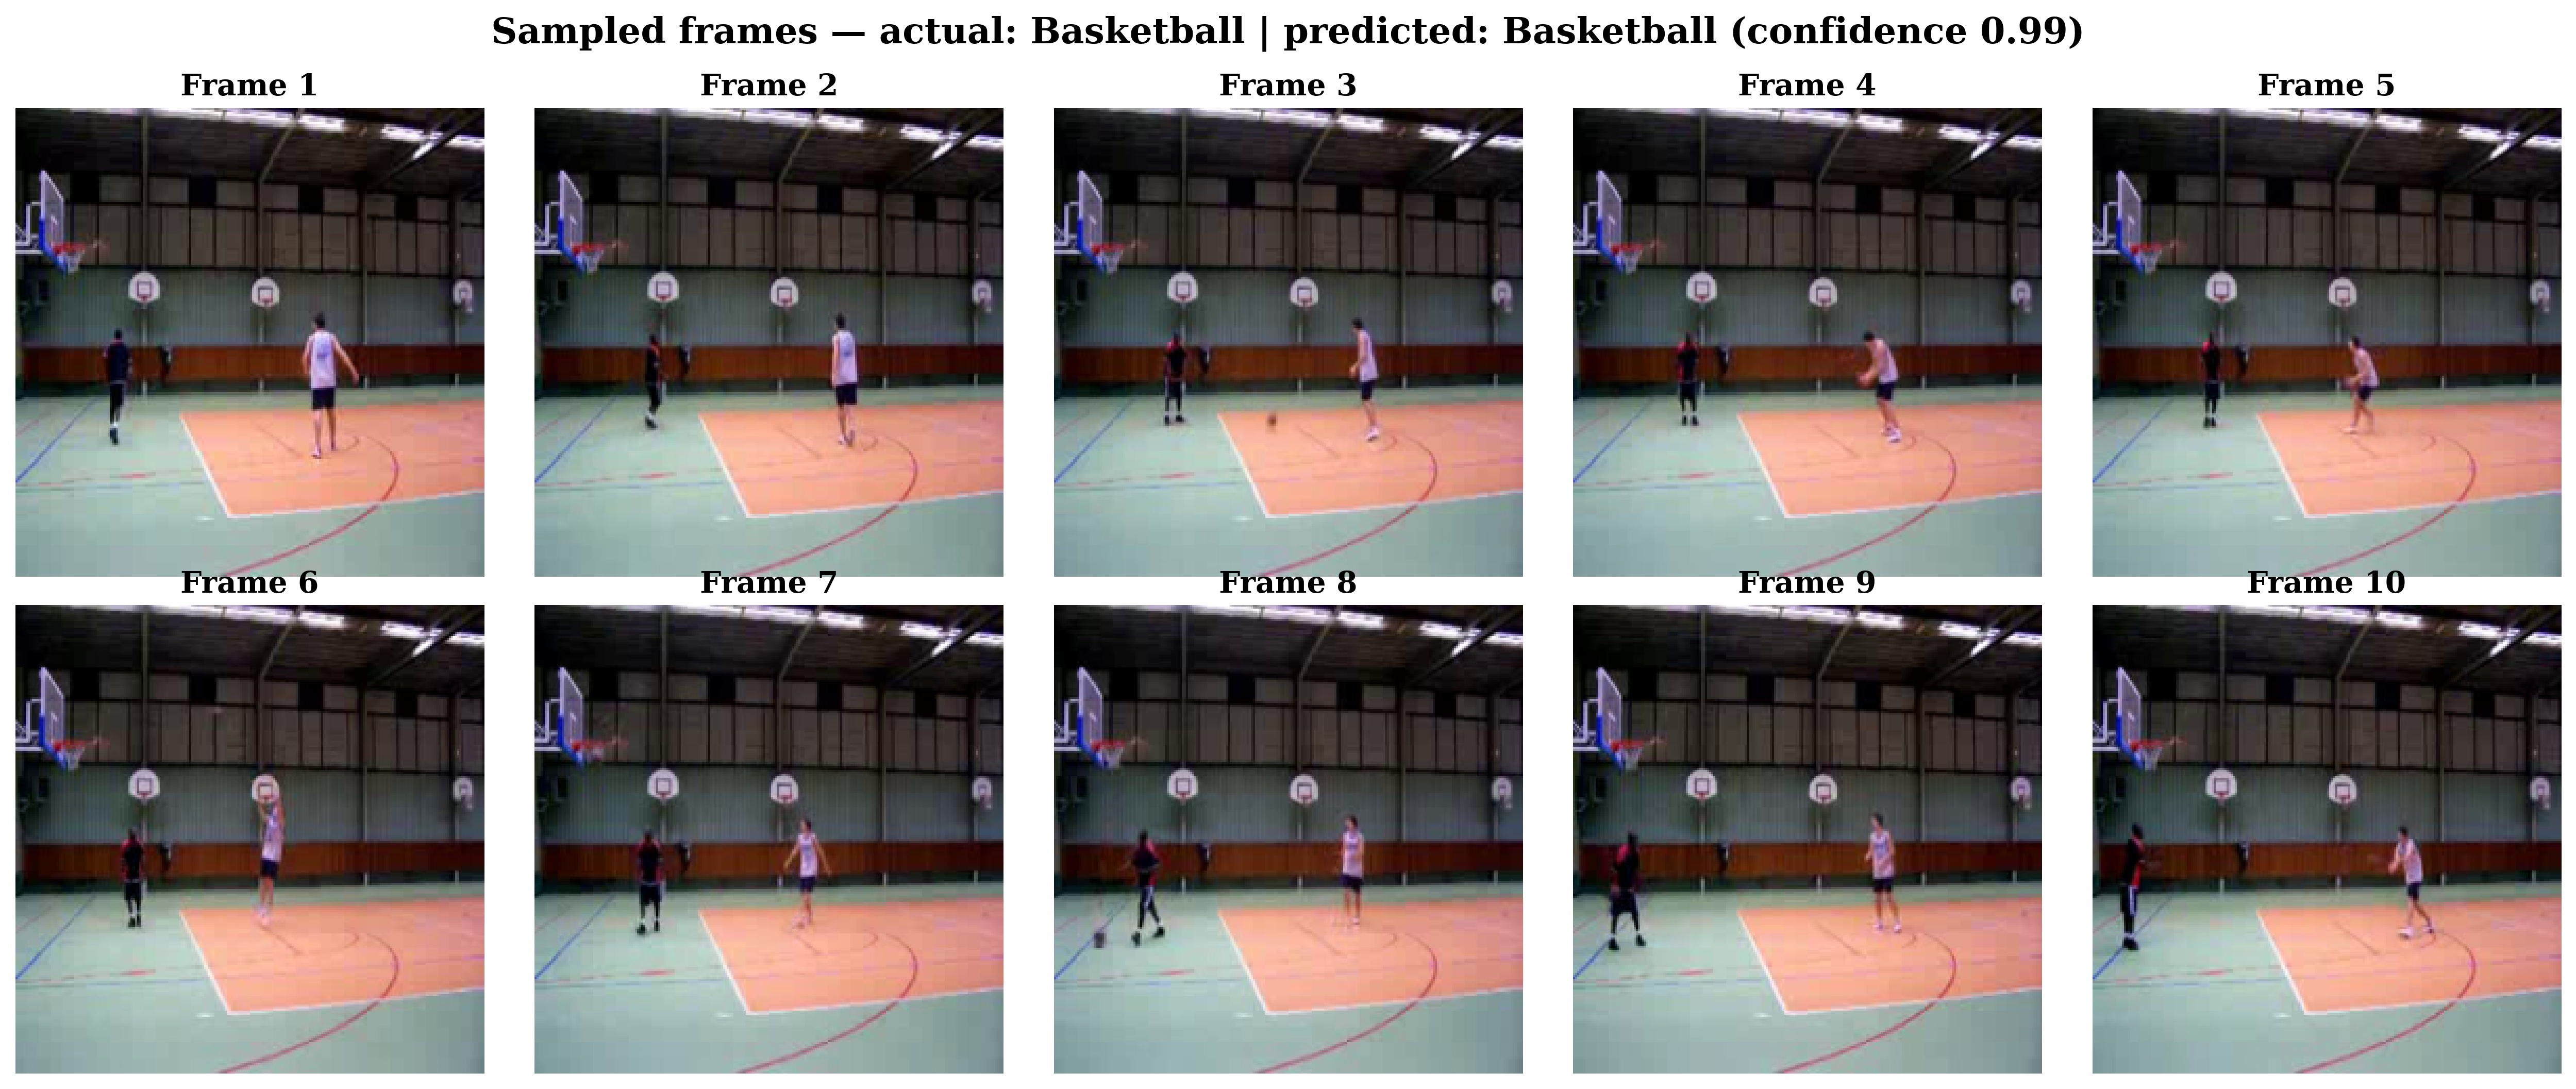
\includegraphics[width=0.95\textwidth]{plot07_video_sample_frames.png}
\caption{Plot 7: 10 uniformly sampled $224\times224$ frames of a test video (actual class Basketball, predicted Basketball).}
\end{figure}

\textbf{Inference:} 10 frames ($224\times224$) of a `Basketball' video --
the CNN gives one 1280-d vector per frame encoding objects, scene and pose
(spatial information). The LSTM/GRU reads the 10 vectors in order and
learns how they change (motion, repetition) -- the temporal information a
single frame cannot give.

\begin{figure}[H]
\centering
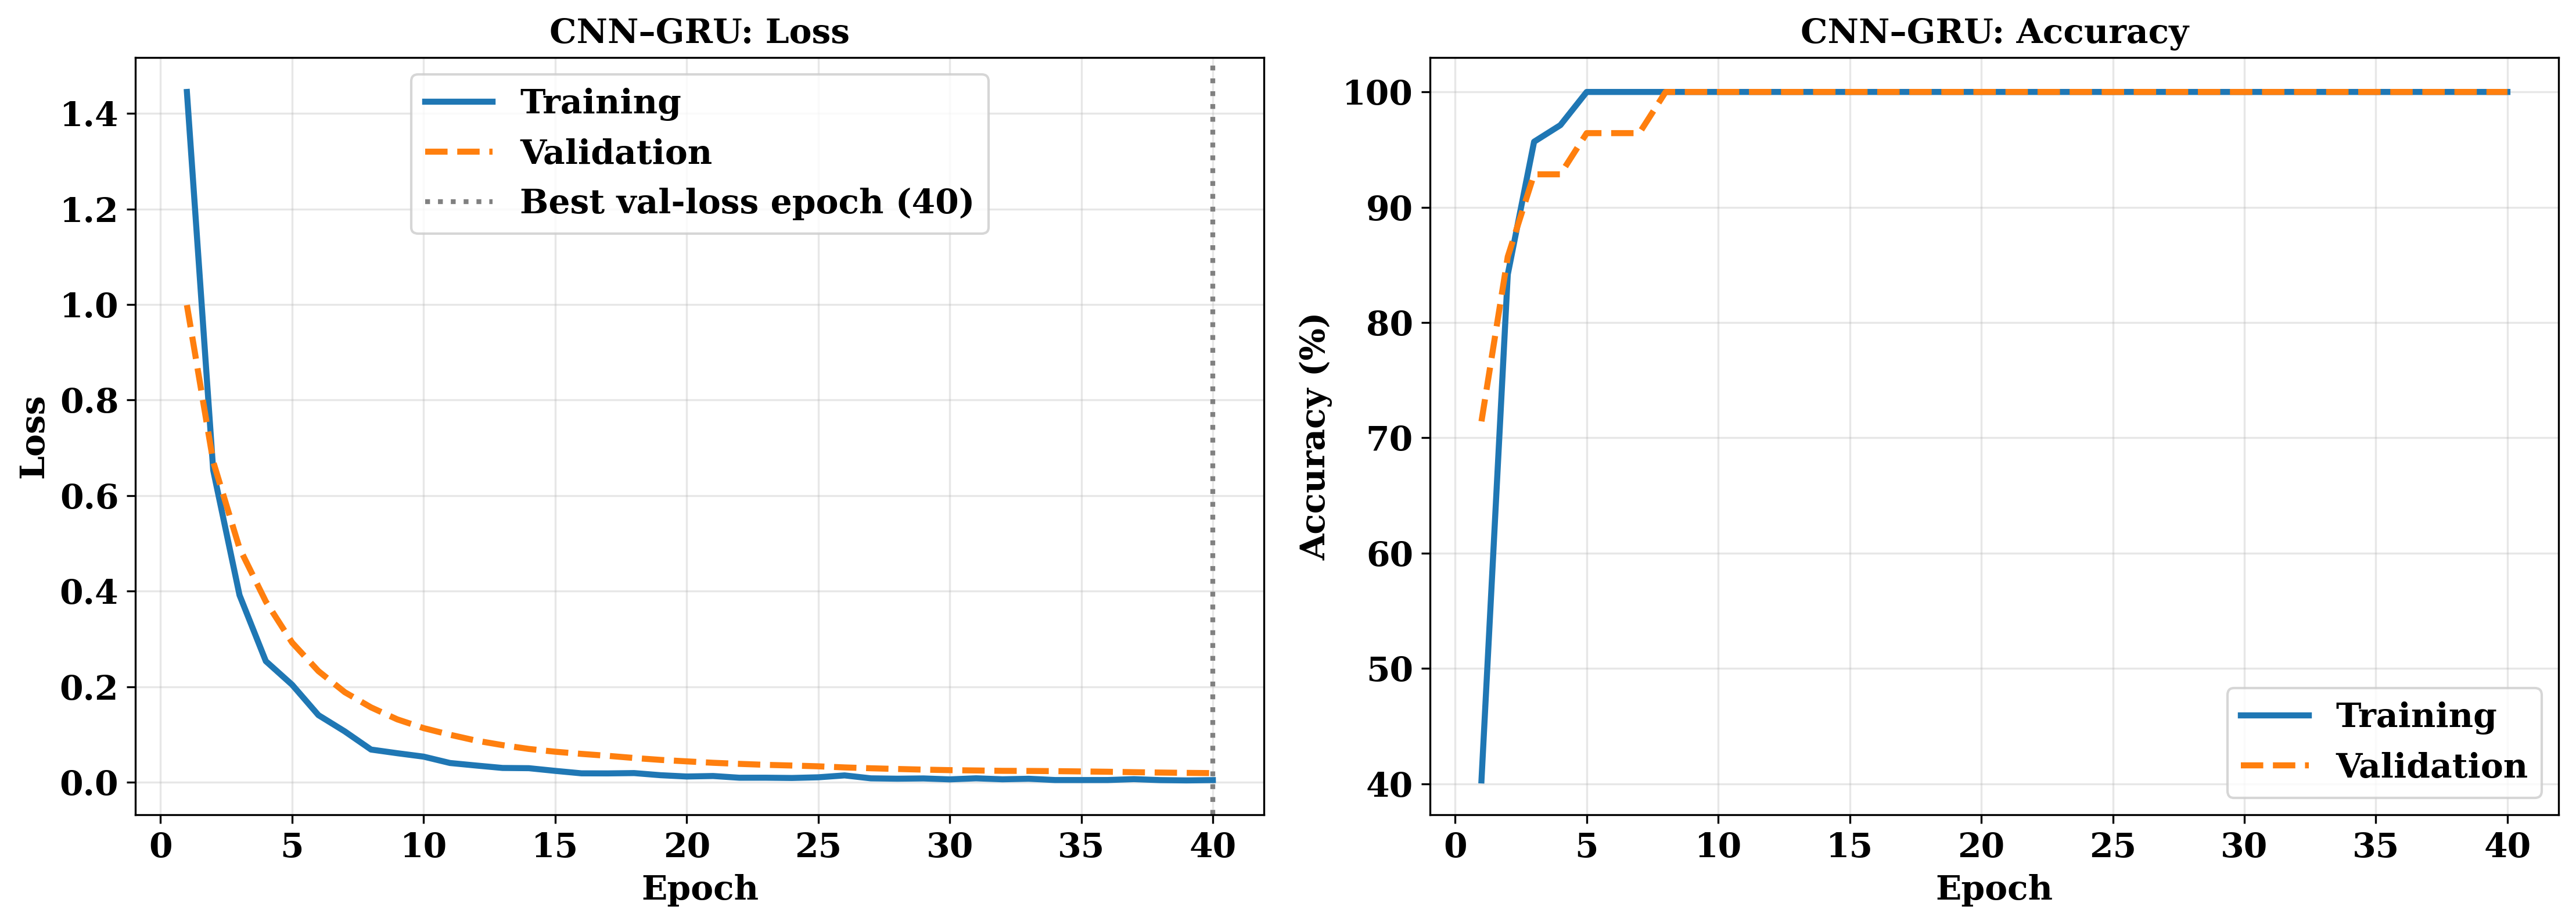
\includegraphics[width=0.9\textwidth]{plot08_video_training_curves.png}
\caption{Plot 8: CNN--GRU training/validation loss and accuracy versus epoch.}
\end{figure}

\textbf{Inference:} CNN--GRU: train loss $1.44\rightarrow0.00$, val loss
minimum $0.02$ at epoch 40/40; final train/val accuracy $100\%/100\%$.
Still converging by the last epoch -- with only 139 training / 28
validation videos the curves are noisy, but the frozen ImageNet features
make learning very fast.

\begin{figure}[H]
\centering
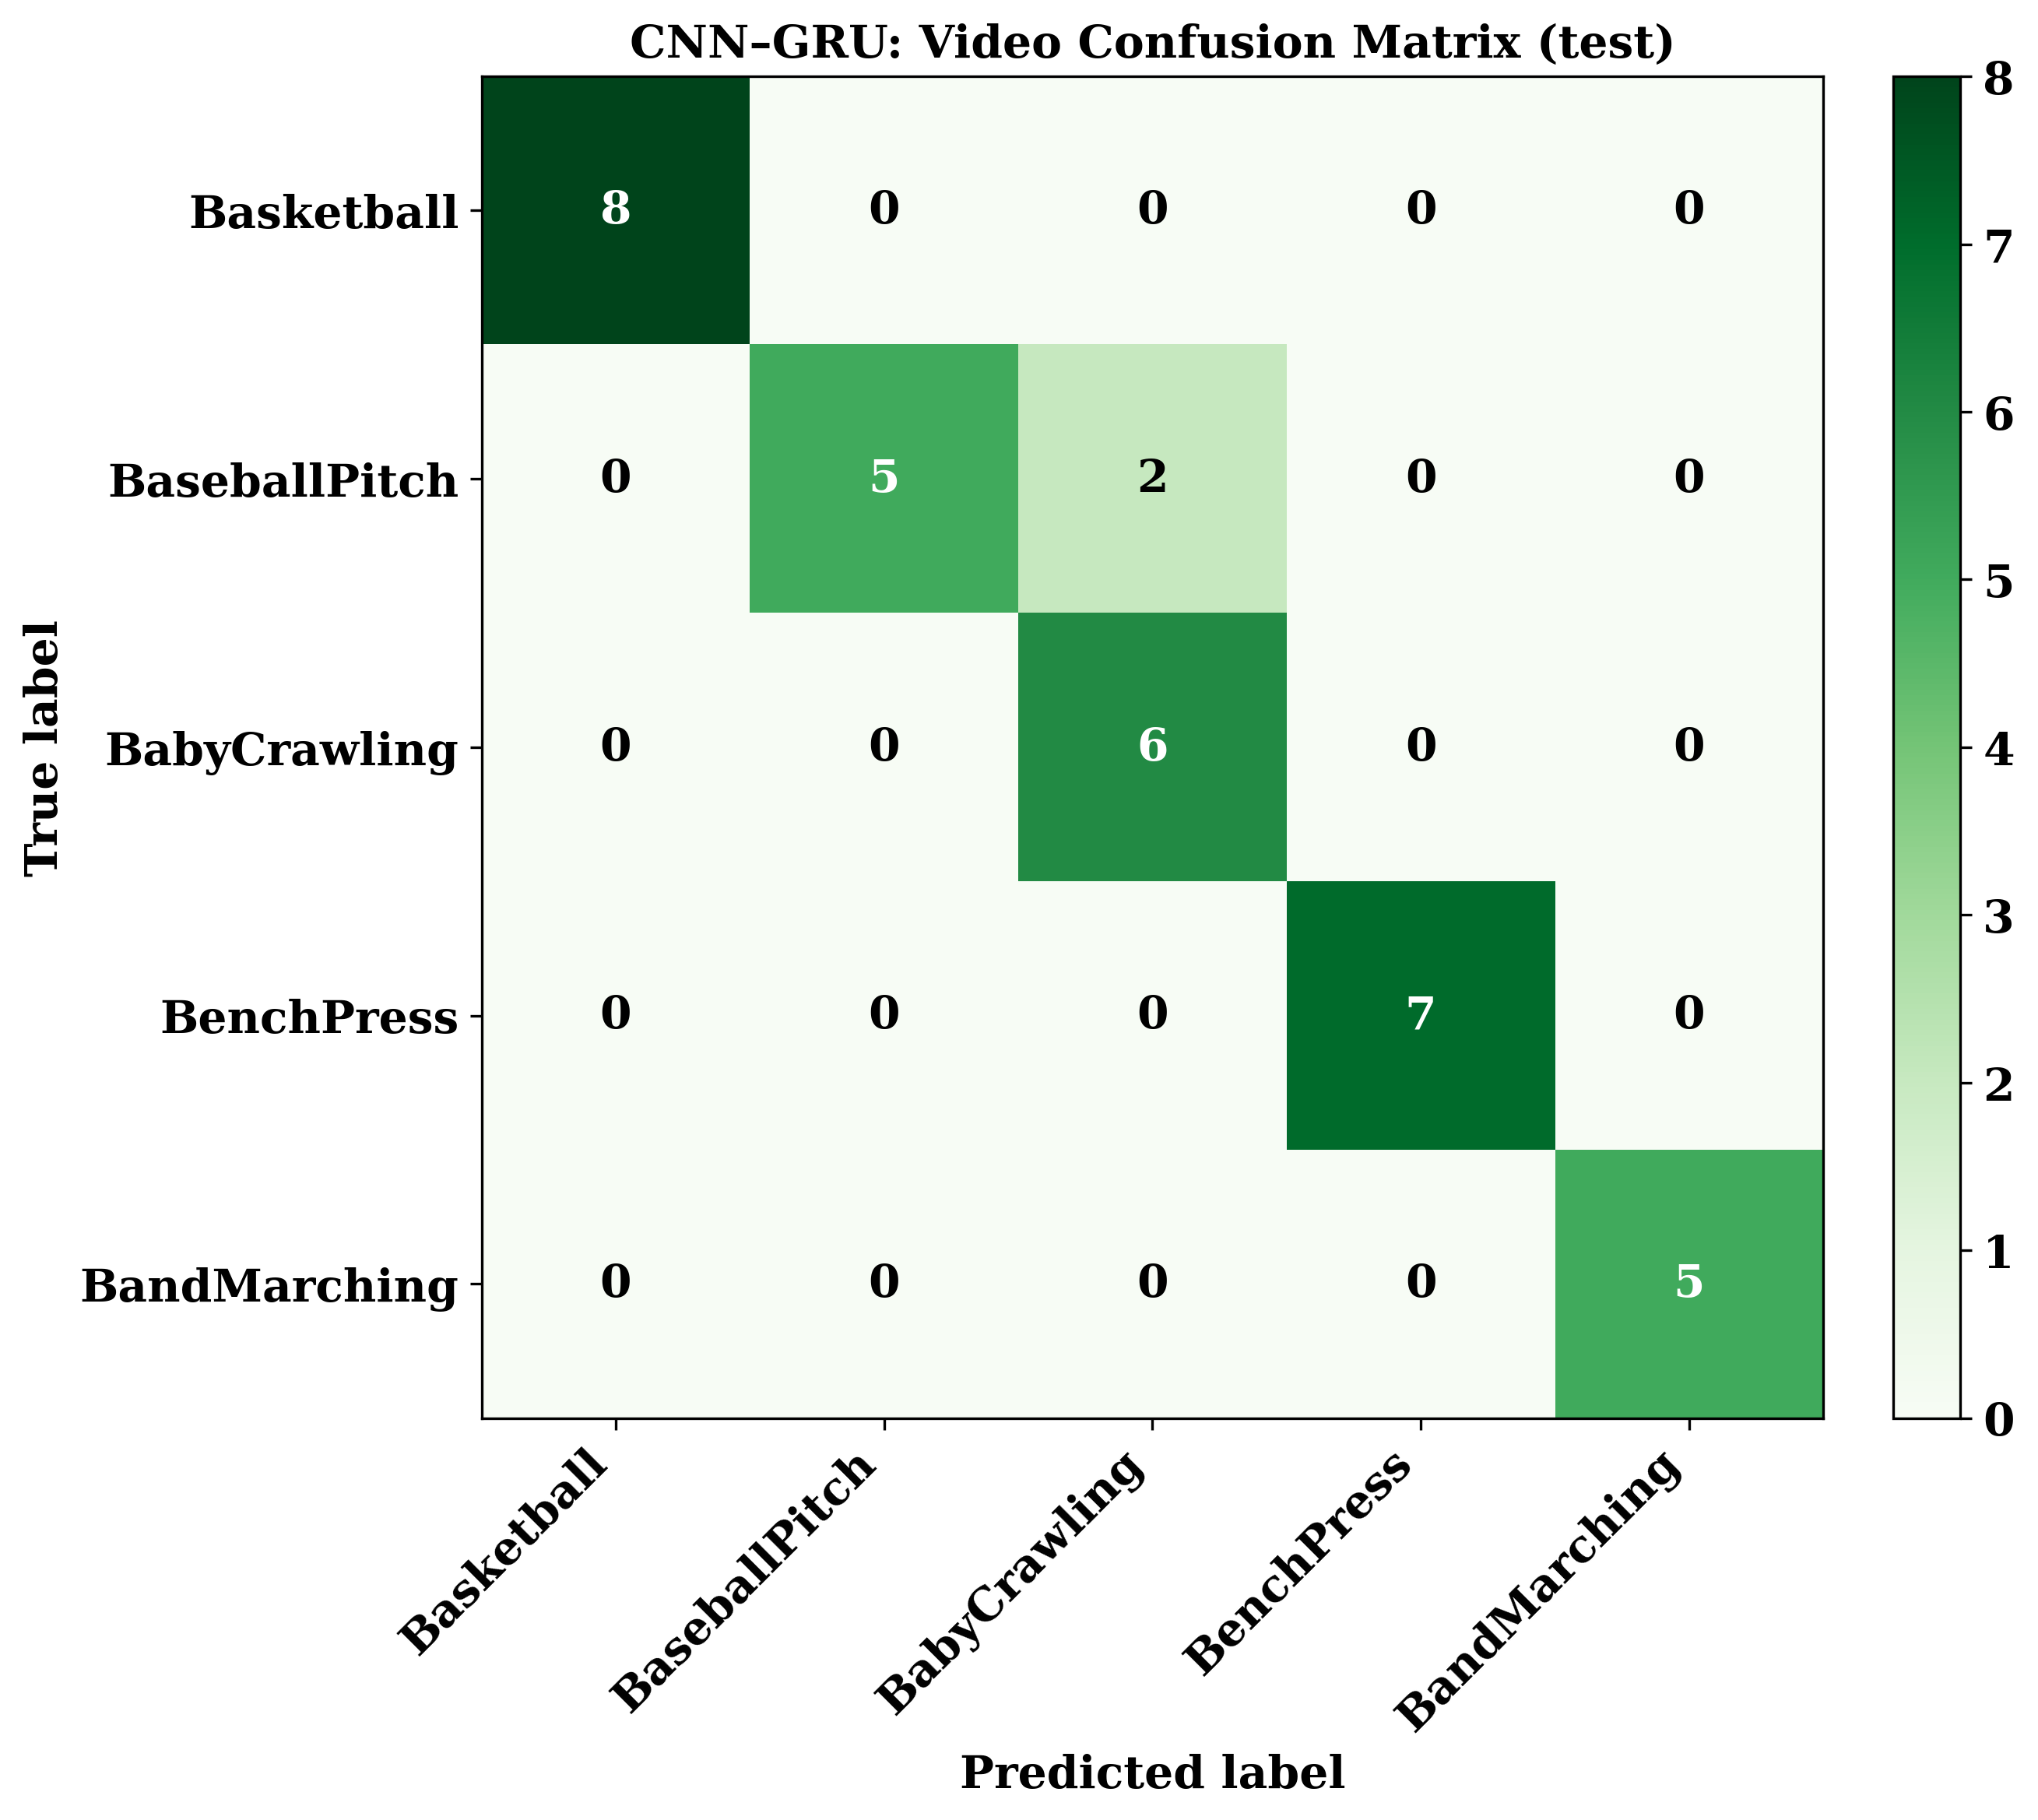
\includegraphics[width=0.6\textwidth]{plot09_video_confusion.png}
\caption{Plot 9: CNN--GRU video confusion matrix (test set).}
\end{figure}

\textbf{Inference:} CNN--GRU: best class Basketball (100\%); most errors on
BaseballPitch (2 errors, recall 71\%). Top confusion: BaseballPitch
$\leftrightarrow$ BabyCrawling (2 samples) -- similar scenes/motion in the
sampled frames.

%%%%%%%%%%%%%%%%%%%%%%%%%%%%%%%%%%%%%%%%%%%%%%%%%%%%%%%%%%%%
\section*{22. Sequence-to-Sequence Learning}

Sequence-to-sequence learning maps one sequence to another.

For a simple laboratory task, construct a synthetic reversal dataset.

Example:

\[
[1,4,7,2]\rightarrow[2,7,4,1].
\]

Generate several thousand short sequences using integers from a fixed range.

The task is intentionally simple so that the encoder--decoder mechanism can
be studied without a large external dataset.

\begin{center}
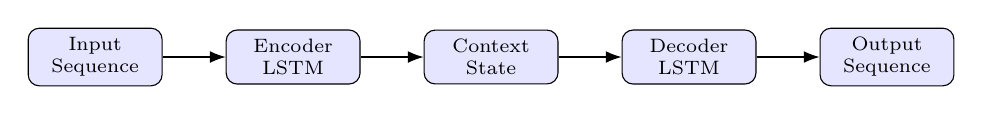
\begin{tikzpicture}[node distance=8mm]
\node[layer](a){Input\\Sequence};
\node[layer,right=of a](b){Encoder\\LSTM};
\node[layer,right=of b](c){Context\\State};
\node[layer,right=of c](d){Decoder\\LSTM};
\node[layer,right=of d](e){Output\\Sequence};

\foreach \x/\y in {a/b,b/c,c/d,d/e}
\draw[arrow](\x)--(\y);
\end{tikzpicture}
\end{center}

The encoder converts the input sequence into a learned representation.
The decoder generates the output sequence one element at a time.

%%%%%%%%%%%%%%%%%%%%%%%%%%%%%%%%%%%%%%%%%%%%%%%%%%%%%%%%%%%%
\section*{23. Expected Sequence-to-Sequence Input and Output}

\textbf{Input example:}

\[
[3,8,1,5]
\]

\textbf{Expected output:}

\[
[5,1,8,3].
\]

Students must display at least five test examples in the report.

\begin{center}
\begin{tabular}{|c|c|c|c|c|}
\hline
Sample & Input Sequence & Expected Output & Predicted Output & Correct\\
\hline
1 & [7, 9, 9, 1, 2, 8] & [8, 2, 1, 9, 9, 7] & [8, 2, 1, 9, 9, 7] & \checkmark\\
2 & [3, 4, 9, 8, 4, 6] & [6, 4, 8, 9, 4, 3] & [6, 4, 8, 9, 4, 3] & \checkmark\\
3 & [8, 9, 9, 9, 4, 2] & [2, 4, 9, 9, 9, 8] & [2, 4, 9, 9, 9, 8] & \checkmark\\
4 & [2, 2, 8, 6, 6, 9] & [9, 6, 6, 8, 2, 2] & [9, 6, 6, 8, 2, 2] & \checkmark\\
5 & [9, 5, 4, 5, 6, 5] & [5, 6, 5, 4, 5, 9] & [5, 6, 5, 4, 5, 9] & \checkmark\\
\hline
6 (error case) & [8, 1, 1, 1, 1, 1] & [1, 1, 1, 1, 1, 8] & [1, 1, 1, 1, 1, 9] & $\times$\\
\hline
\end{tabular}
\end{center}

(An additional error case is shown to illustrate the rare failure mode: a
digit that repeats five times in the input is occasionally mispredicted at
one position.)

\subsection*{Observed Results (Model Configuration)}

12{,}000 unique length-6 sequences over integers 1--9 were generated and
split into 8{,}399 train / 1{,}801 validation / 1{,}800 test sequences (no
overlap). The encoder--decoder (LSTM, 128 units, embedding dimension 32) has
500{,}384 total parameters (166{,}794 trainable in the training graph) and
was trained for 60 epochs with teacher forcing:

\begin{verbatim}
epoch  1  | loss 2.0034  acc  25.0% | val_loss 1.6154  val_acc  37.7%
epoch  10 | loss 0.0164  acc 100.0% | val_loss 0.0150  val_acc 100.0%
epoch  30 | loss 0.0014  acc 100.0% | val_loss 0.0016  val_acc 100.0%
epoch  60 | loss 0.0003  acc 100.0% | val_loss 0.0004  val_acc 100.0%
\end{verbatim}

%%%%%%%%%%%%%%%%%%%%%%%%%%%%%%%%%%%%%%%%%%%%%%%%%%%%%%%%%%%%
\section*{24. Sequence-to-Sequence Evaluation}

Report:

\begin{itemize}
\item Token accuracy
\item Sequence accuracy
\item Training loss
\item Validation loss
\end{itemize}

Token accuracy is

\[
\text{Token Accuracy}
=
\frac{\text{Correctly predicted tokens}}
{\text{Total tokens}}.
\]

Sequence accuracy is

\[
\text{Sequence Accuracy}
=
\frac{\text{Completely correct sequences}}
{\text{Total sequences}}.
\]

\subsection*{Observed Results}

\begin{center}
\begin{tabular}{|l|c|}
\hline
Metric & Value\\
\hline
Token accuracy & 99.99\%\\
Sequence accuracy & 99.94\%\\
Training loss & 0.0003\\
Validation loss & 0.0004\\
Parameters & 166,794\\
Training time & 44.9 s\\
\hline
\end{tabular}
\end{center}

\begin{figure}[H]
\centering
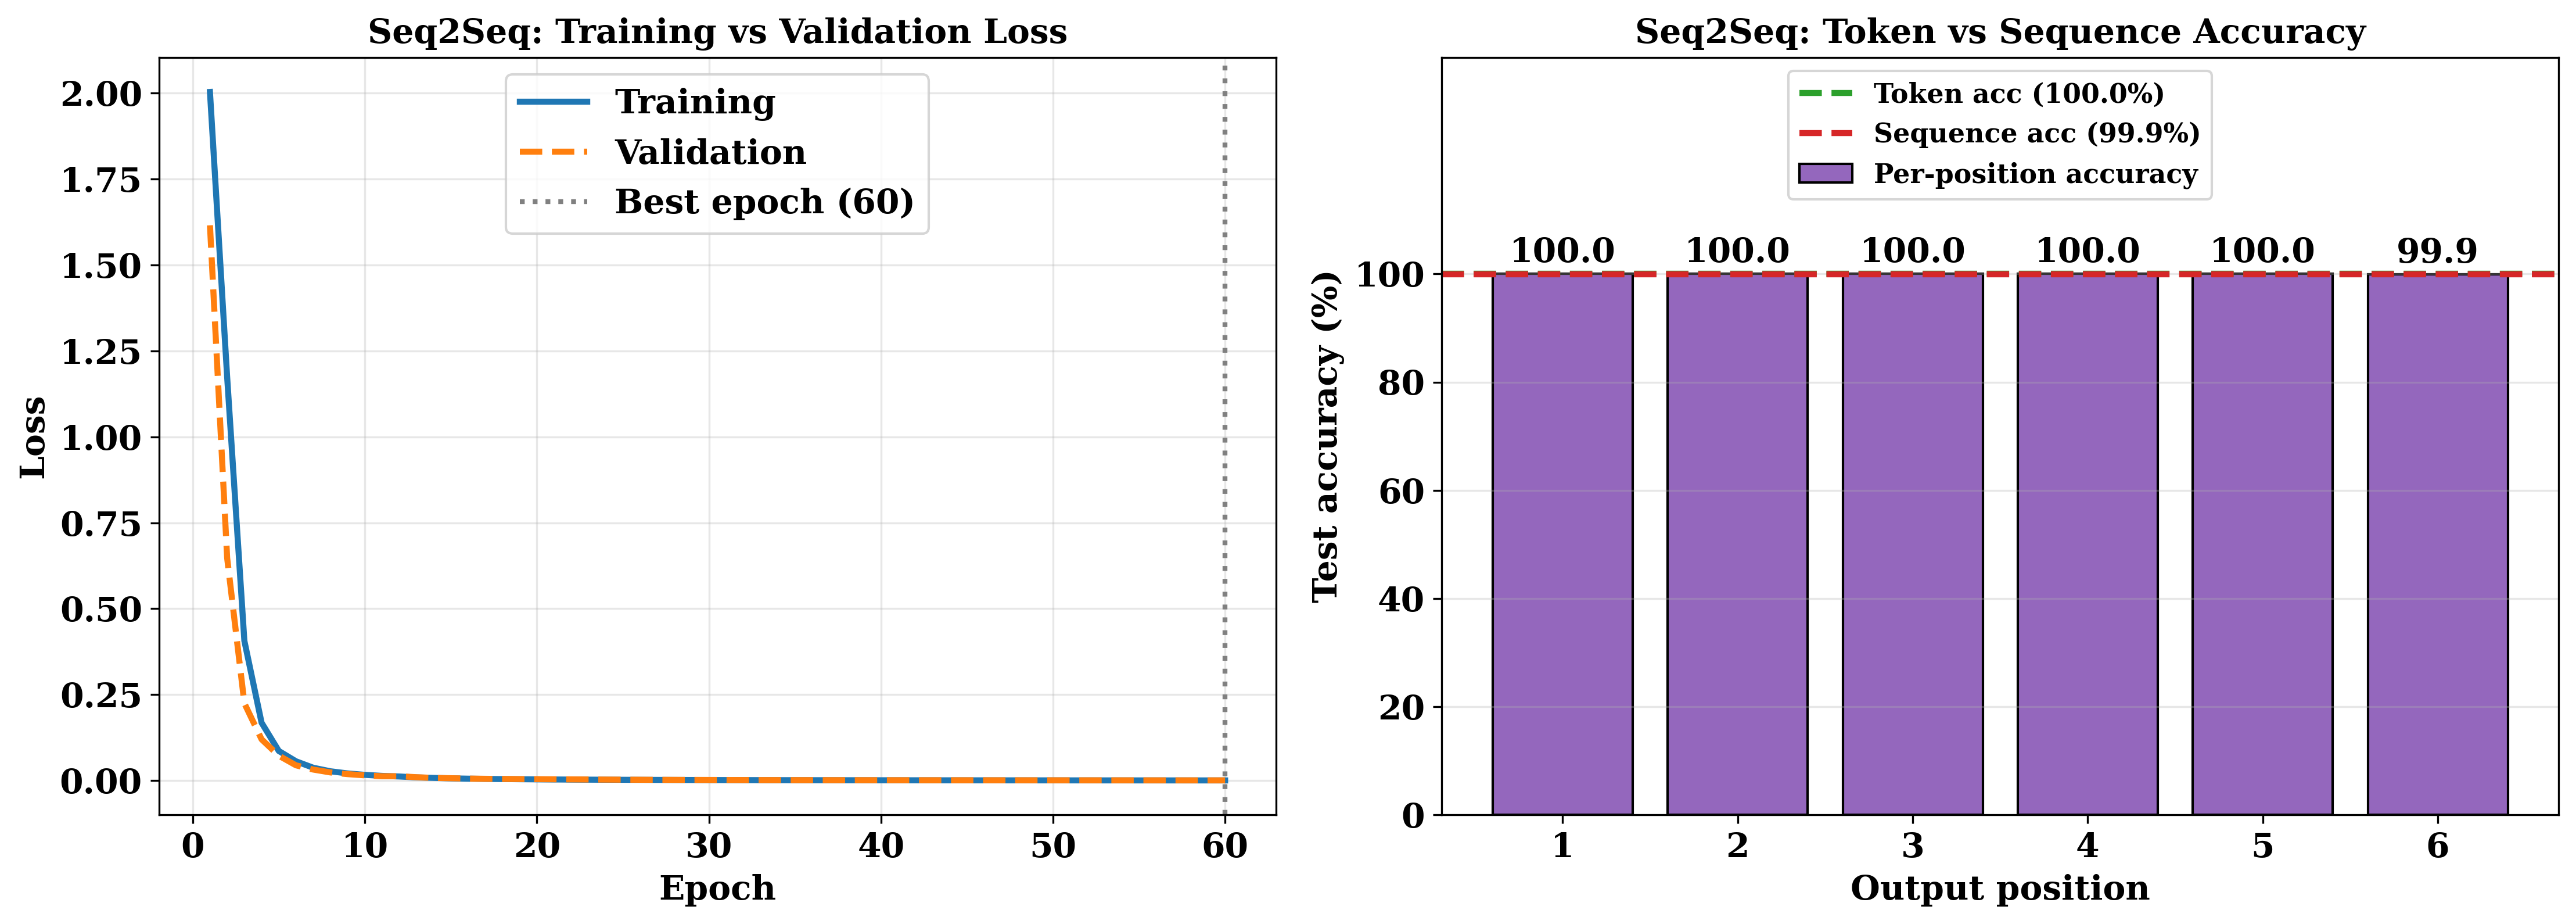
\includegraphics[width=0.95\textwidth]{plot10_seq2seq_loss_and_accuracy.png}
\caption{Plot 10 (loss curve): training/validation loss versus epoch (left); token vs.\ sequence accuracy by output position (right).}
\end{figure}

\textbf{Inference:} Best epoch 60/60: train loss $0.000$, val loss $0.000$
(teacher forcing: true previous tokens used as decoder input). At test time
the decoder feeds back its own output: token accuracy $100.0\%$ vs sequence
accuracy $99.9\%$.

\textbf{Inference (token vs.\ sequence accuracy):} One wrong token spoils
the whole sequence: token accuracy $100.0\%\rightarrow\approx99.9\%$ if
errors were independent (observed $99.9\%$). Accuracy by output position
ranges $100$--$100\%$ (position 6 hardest); because a wrong token is fed
back into the decoder, sequence accuracy is always $\le$ token accuracy.

%%%%%%%%%%%%%%%%%%%%%%%%%%%%%%%%%%%%%%%%%%%%%%%%%%%%%%%%%%%%
\section*{25. Consolidated Results}

Students must complete the following table.

\begin{center}
\begin{tabular}{|l|c|c|c|c|c|}
\hline
Model & Accuracy (\%) & Precision (\%) & Recall (\%) & F1 (\%) & Parameters\\
\hline
RNN & 72.16 & 72.80 & 74.42 & 73.03 & 1,974\\
LSTM & 94.86 & 95.45 & 94.93 & 94.84 & 6,006\\
GRU & 98.29 & 98.42 & 98.23 & 98.29 & 4,758\\
CNN--GRU (video) & 93.94 & 95.00 & 94.29 & 93.81 & 127,365\\
\hline
\end{tabular}
\end{center}

A separate table must be provided for the sequence-to-sequence task.

\subsection*{Observed Results}

\begin{center}
\begin{tabular}{|l|c|c|c|c|c|c|}
\hline
Token Acc. & Sequence Acc. & Training Loss & Validation Loss & Parameters & Training Time\\
\hline
99.99\% & 99.94\% & 0.0003 & 0.0004 & 166,794 & 44.9 s\\
\hline
\end{tabular}
\end{center}

%%%%%%%%%%%%%%%%%%%%%%%%%%%%%%%%%%%%%%%%%%%%%%%%%%%%%%%%%%%%
\section*{26. Discussion Questions}

\begin{enumerate}
\item What is a recurrent neural network?

\textbf{Answer:} A recurrent neural network is a network with a feedback
loop: at each step it combines the current input with a hidden state
carried from the previous step, using the same weights at every step, so it
can process variable-length sequences.

\item What information is represented by the hidden state?

\textbf{Answer:} The hidden state represents a compressed summary of
everything seen so far in the sequence (its ``memory''), which is passed to
the next step and, at the end, to the classifier.

\item Why is sequence order important?

\textbf{Answer:} Sequence order is important because the meaning lies in
the ordering (gait cycles, posture transitions, words in a sentence, motion
in a video); shuffling the time steps destroys these patterns although the
individual values stay the same.

\item Explain the difference between a feed-forward network and an RNN.

\textbf{Answer:} A feed-forward network maps a fixed-size input to an
output with no memory and independent inputs; an RNN reuses its weights
over time and has a recurrent connection $h_{t-1}\to h_t$, so its output
depends on the whole history.

\item Explain Backpropagation Through Time.

\textbf{Answer:} Backpropagation Through Time unrolls the RNN over $T$
steps (a deep network with shared weights), runs the forward pass, then
backpropagates the loss through every step and sums the weight gradients
from all steps.

\item Why can gradients vanish during BPTT?

\textbf{Answer:} Gradients can vanish during BPTT because the gradient
reaching step $t-k$ contains a product of $k$ Jacobians
$\operatorname{diag}(1-h^2)W_h$; when their norm is below 1 (saturating
tanh derivatives $\le1$, small $W_h$) the product shrinks exponentially
with $k$.

\item Why can gradients explode during BPTT?

\textbf{Answer:} Gradients can explode if the norm of those Jacobians is
above 1 (large $W_h$), causing the product to grow exponentially, which
leads to huge updates and unstable training; gradient clipping is the usual
remedy.

\item What are long-term dependencies?

\textbf{Answer:} Long-term dependencies are situations where the output at
a late time step depends on information from many steps earlier; plain
RNNs struggle to learn them because of vanishing gradients.

\item What is the role of the LSTM cell state?

\textbf{Answer:} The LSTM cell state is a separate memory line updated
additively ($C_t=f_tC_{t-1}+i_t\tilde{C}_t$), so information and gradients
can flow across many steps almost unchanged.

\item What are the forget, input and output gates in LSTM?

\textbf{Answer:} The forget gate controls how much of the old cell state to
keep; the input gate controls how much of the new candidate to write; the
output gate controls how much of the (squashed) cell state to expose as
$h_t$.

\item What are the reset and update gates in GRU?

\textbf{Answer:} The reset gate $r_t$ controls how much of the previous
state is used when forming the candidate; the update gate $z_t$ controls
how much of the state is replaced by the candidate versus kept.

\item Compare LSTM and GRU.

\textbf{Answer:} LSTM has separate cell and hidden states, 3 gates, and
more parameters (4 weight blocks). GRU has one state, 2 gates, and fewer
parameters (3 blocks), and is usually faster; accuracy is often similar,
and which wins depends on the data (see the tables above).

\item Why does GRU generally use a simpler gating mechanism than LSTM?

\textbf{Answer:} GRU uses a simpler gating mechanism because it merges the
forget and input gates into one update gate and merges the cell and hidden
state, giving a cheaper unit that keeps most of the long-term-memory
benefit.

\item Why should RNN, LSTM and GRU be compared using the same experimental settings?

\textbf{Answer:} RNN, LSTM and GRU should be compared using the same
experimental settings so that differences in results can be attributed to
the recurrent cell itself and not to different data splits, optimizers,
learning rates, epochs or seeds (a controlled experiment).

\item What does the confusion matrix reveal that accuracy alone does not?

\textbf{Answer:} The confusion matrix reveals which classes are confused
with which, class-wise recall/precision and systematic error patterns
(e.g.\ Sitting $\leftrightarrow$ Standing), which a single accuracy number
hides, especially with class imbalance.

\item Why should macro F1-score be reported for multi-class classification?

\textbf{Answer:} Macro F1-score should be reported because it averages the
per-class F1 with equal weight, so poor performance on a minority or
difficult class is not hidden by frequent classes, and it balances
precision and recall.

\item What is the significance of sequence length?

\textbf{Answer:} Sequence length sets how much temporal context the model
sees, and it also sets the BPTT depth and computational cost: too short
misses the pattern, too long increases cost and gradient problems.

\item Why can a CNN be used as a feature extractor for video?

\textbf{Answer:} A CNN can be a feature extractor for video because a CNN
pretrained on a large image dataset (ImageNet) already encodes generic
visual concepts; with the classification head removed it turns every frame
into a compact vector without training a CNN from scratch on a small video
set.

\item What type of information is extracted by the CNN?

\textbf{Answer:} The CNN extracts spatial information in a single frame:
edges, textures, objects, body shape/pose and scene context.

\item What type of information is learned by the recurrent network?

\textbf{Answer:} The recurrent network learns temporal information across
frames: how the spatial features change (motion, repetition, order of
events), which decides the action.

\item Why are CNN features arranged as a sequence before being given to LSTM/GRU?

\textbf{Answer:} CNN features are arranged as a sequence because frames are
ordered in time; stacking the per-frame vectors in order gives a $(T,D)$
sequence, the input format LSTM/GRU expect, so temporal relations can be
modelled.

\item Explain the encoder and decoder in sequence-to-sequence learning.

\textbf{Answer:} The encoder reads the input sequence and compresses it
into a context (its final state); the decoder is initialised with this
context and generates the output sequence one token at a time, feeding back
the previous token.

\item What is teacher forcing?

\textbf{Answer:} Teacher forcing means that during training the decoder
receives the ground-truth previous token instead of its own previous
prediction; this speeds up and stabilises training but creates a
train/test mismatch (exposure bias) because at test time it must use its
own outputs.

\item Differentiate token accuracy and sequence accuracy.

\textbf{Answer:} Token accuracy is the fraction of individual tokens
predicted correctly; sequence accuracy is the fraction of sequences with
\emph{all} tokens correct. The second is always $\le$ the first, since one
wrong token invalidates a whole sequence.

\item Why must the test set remain untouched during model selection?

\textbf{Answer:} The test set must remain untouched during model selection
because if it influences choices (epochs, hyperparameters, architecture),
the reported score becomes optimistically biased; selection must use the
validation set so that the test set gives an unbiased estimate of
generalisation.
\end{enumerate}

%%%%%%%%%%%%%%%%%%%%%%%%%%%%%%%%%%%%%%%%%%%%%%%%%%%%%%%%%%%%
\section*{27. Additional Exercises}

\begin{enumerate}
\item Replace the 32 recurrent units with 16 and 64 units and study the effect
on accuracy, F1-score, parameter count and training time.
\item Compare GRU and LSTM using the same number of recurrent units.
\item Add a second recurrent layer and investigate whether performance improves.
\item Compare a bidirectional LSTM with a unidirectional LSTM.
\item Change the sequence length and study the effect on computational cost.
\item For the video task, compare LSTM and GRU after extracting identical CNN
features.
\item Modify the seq2seq task so that the output sequence has a different
length from the input sequence.
\end{enumerate}

\subsection*{Observed Results}

\textbf{Exercises 1, 3 and 4 (units, depth, bidirectionality):}

\begin{center}
\begin{tabular}{|l|c|c|c|c|c|c|}
\hline
Model & Units & Layers & Bidirectional & Accuracy (\%) & Macro F1 (\%) & Parameters\\
\hline
LSTM-16u-1L & 16 & 1 & No & 97.43 & 97.42 & 2,038\\
LSTM-32u-1L & 32 & 1 & No & 94.86 & 94.84 & 6,006\\
LSTM-64u-1L & 64 & 1 & No & 96.15 & 96.02 & 20,086\\
GRU-16u-1L & 16 & 1 & No & 97.22 & 97.27 & 1,670\\
GRU-32u-1L & 32 & 1 & No & 98.29 & 98.29 & 4,758\\
GRU-64u-1L & 64 & 1 & No & 99.14 & 99.22 & 15,542\\
LSTM-32u-2L & 32 & 2 & No & 96.79 & 96.65 & 14,326\\
GRU-32u-2L & 32 & 2 & No & 98.93 & 98.90 & 11,094\\
BiLSTM-32u-1L & 32 & 1 & Yes & 94.22 & 94.21 & 11,894\\
\hline
\end{tabular}
\end{center}

\begin{figure}[H]
\centering
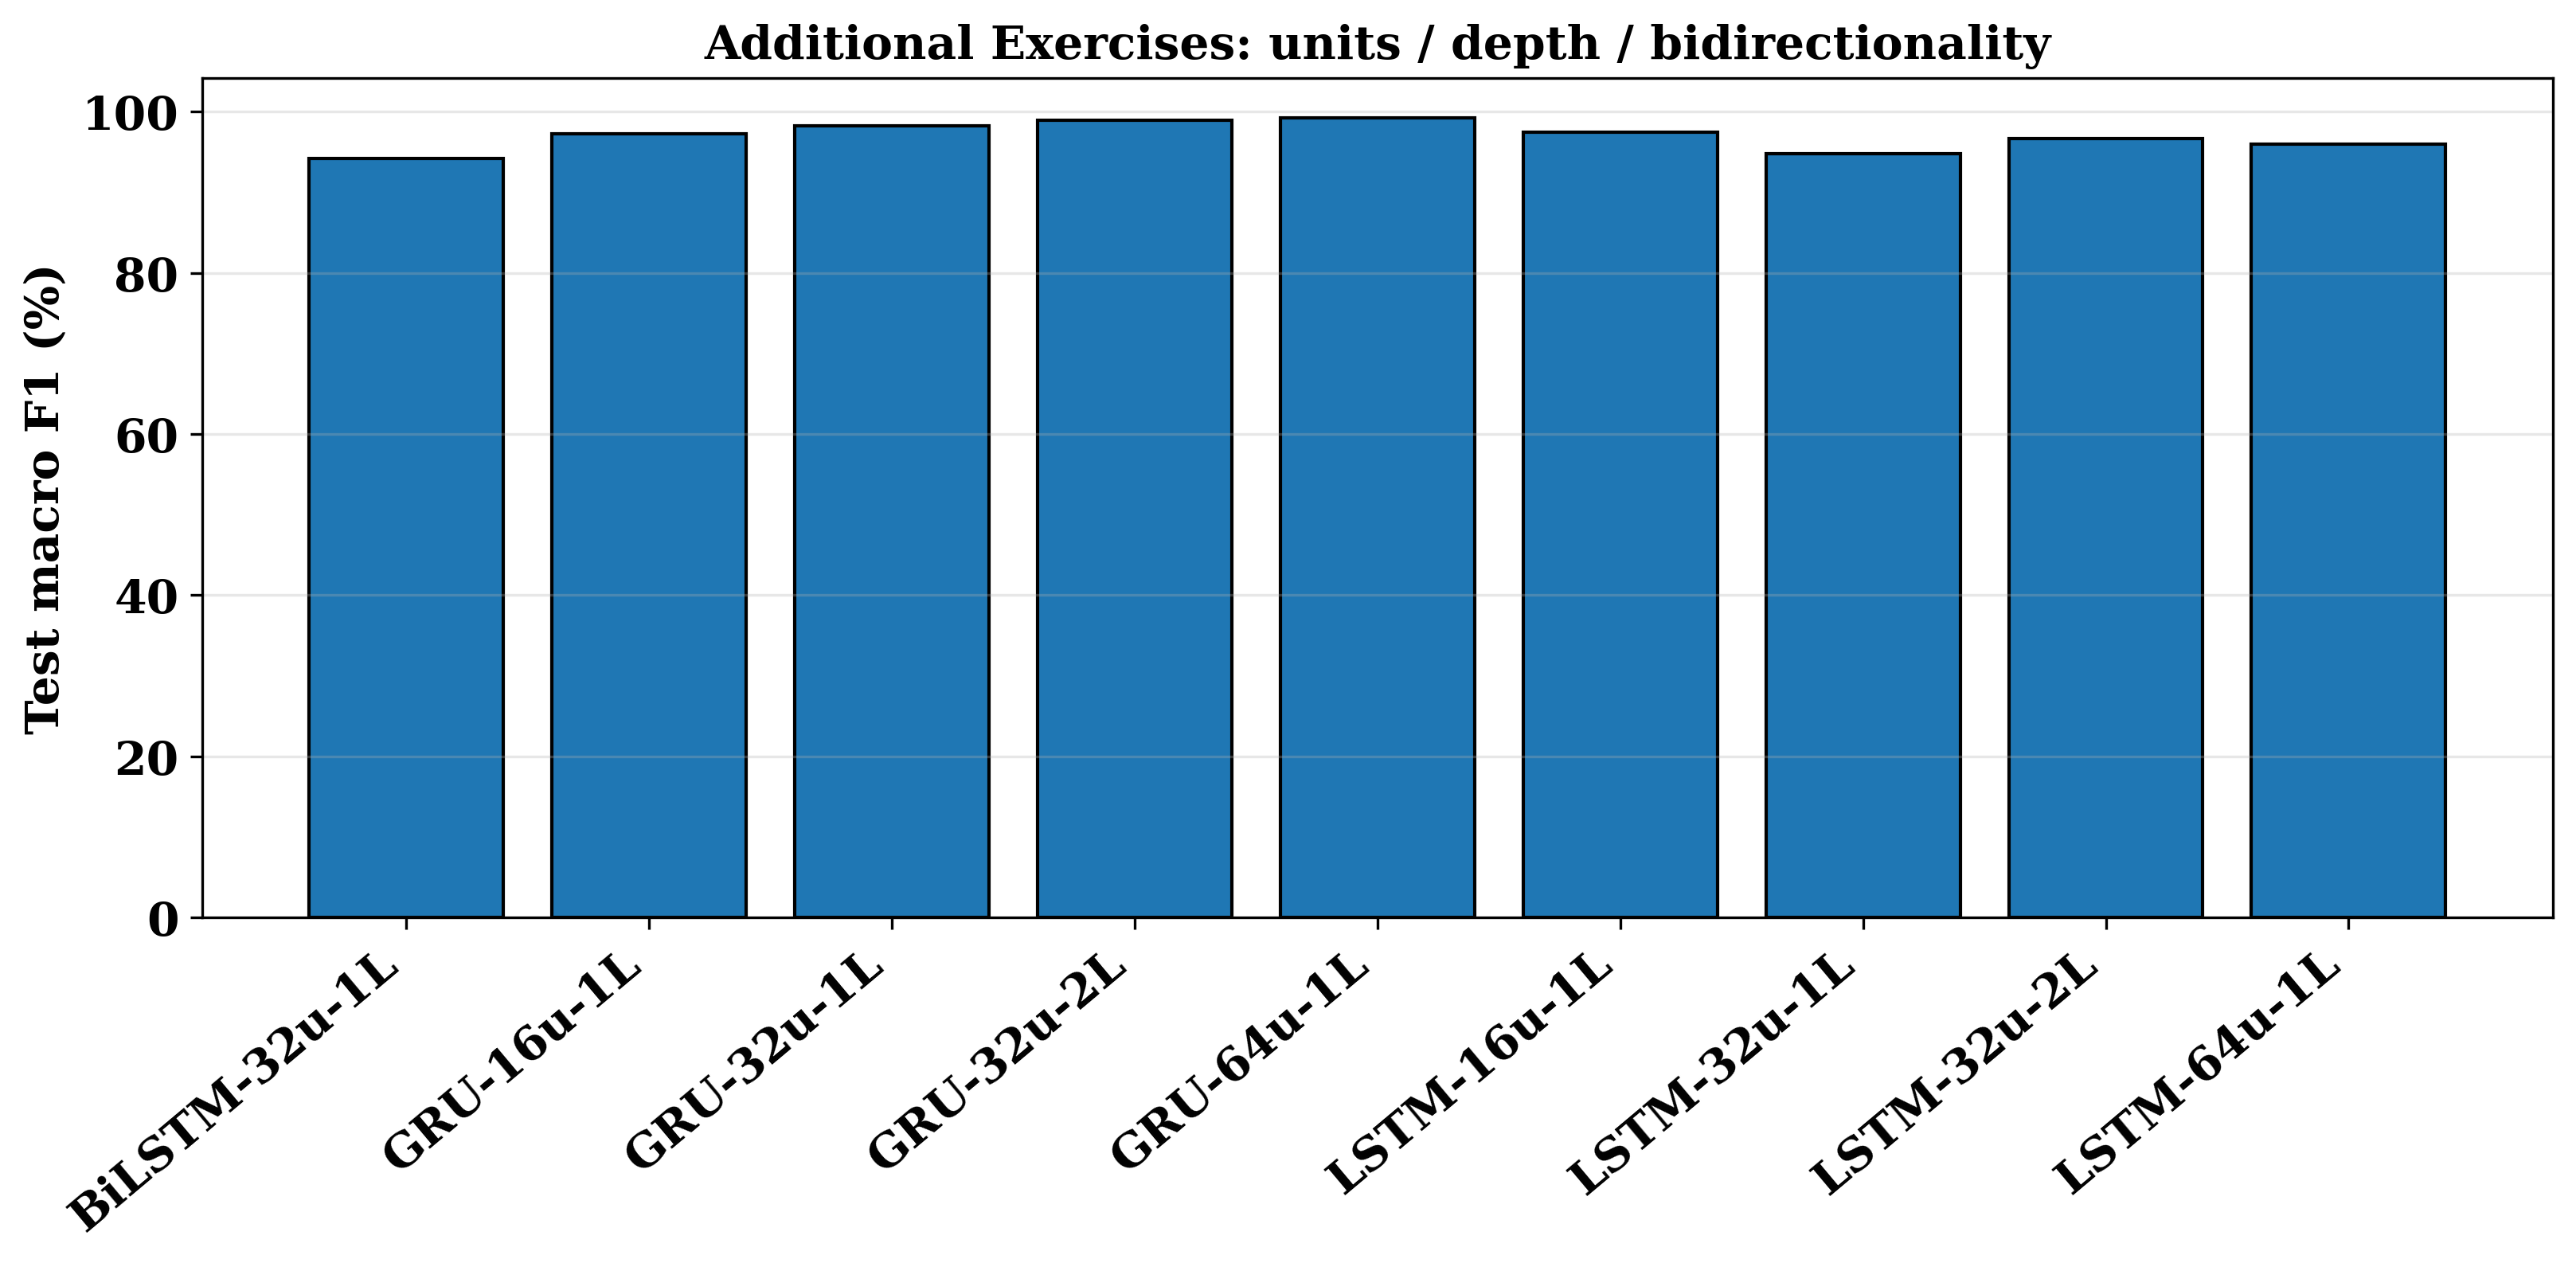
\includegraphics[width=0.75\textwidth]{plot11_additional_exercises.png}
\caption{Plot 11: Test macro F1-score across the additional unit/depth/bidirectionality configurations.}
\end{figure}

\textbf{Inference:} Best configuration by test macro-F1 is GRU-64u-1L
($99.2\%$, 15{,}542 parameters). Extra units, depth or bidirectionality all
increase parameters and training time; here a wider single-layer GRU
(Ex.\,1) beats a deeper 2-layer GRU (Ex.\,3) and the bidirectional LSTM
(Ex.\,4) does not clearly outperform the unidirectional LSTM baseline --
gains should exceed run-to-run noise before adding the extra cost.

\textbf{Exercise 2 (GRU vs.\ LSTM, same units):} Already available at 32
units in Section 14 -- GRU (98.29\% acc, 98.29\% F1, 4{,}758 params)
outperforms LSTM (94.86\% acc, 94.84\% F1, 6{,}006 params) while using
$\sim$21\% fewer parameters.

\textbf{Exercise 5 (sequence length vs.\ cost):} See the training-time table
in Section 17 -- times are roughly similar for $T=32$ and $T=64$
($\sim$20--22 s) and rise for $T=128$ (RNN 30.6 s, LSTM 25.5 s, GRU 26.3 s),
since more time steps mean more sequential computation per epoch.

\textbf{Exercise 6 (video: LSTM vs.\ GRU, identical CNN features):}

\begin{center}
\begin{tabular}{|l|c|c|}
\hline
Metric & CNN--LSTM & CNN--GRU\\
\hline
Test accuracy (\%) & 93.94 & 93.94\\
Macro F1 (\%) & 93.81 & 93.81\\
Parameters & 169,285 & 127,365\\
Training time (s) & 19.87 & 9.69\\
\hline
\end{tabular}
\end{center}

Both recurrent cells reach identical accuracy/F1 on the frozen CNN features,
but GRU trains about twice as fast and uses about 25\% fewer parameters.

\textbf{Exercise 7 (output length $\ne$ input length):} The seq2seq model
was retrained to map a length-6 input to the \emph{first 3} tokens of its
reversal (encoder input length 6, decoder output length 3):

\begin{verbatim}
epoch  1  | loss 1.9477  acc  30.9% | val_loss 1.4279  val_acc  45.5%
epoch  40 | loss 0.0002  acc 100.0% | val_loss 0.0002  val_acc 100.0%

Ex.7 (input length 6 -> output length 3): token acc 100.0% | sequence acc 100.0%
  [1, 6, 3, 9, 3, 5] -> predicted [5, 3, 9] | expected [5, 3, 9]
  [9, 2, 1, 2, 4, 1] -> predicted [1, 4, 2] | expected [1, 4, 2]
  [8, 1, 1, 5, 8, 9] -> predicted [9, 8, 5] | expected [9, 8, 5]
  [2, 8, 1, 1, 8, 7] -> predicted [7, 8, 1] | expected [7, 8, 1]
  [4, 5, 6, 6, 7, 1] -> predicted [1, 7, 6] | expected [1, 7, 6]
\end{verbatim}

The encoder--decoder architecture generalises directly to
different-length outputs since the decoder length is simply the number of
autoregressive steps run, independent of the encoder's input length.

%%%%%%%%%%%%%%%%%%%%%%%%%%%%%%%%%%%%%%%%%%%%%%%%%%%%%%%%%%%%
\section*{28. Expected Outcome}

At the end of the experiment, students should be able to demonstrate the
complete sequence-learning pipeline:

\[
\boxed{
\text{Sequential Data}
\rightarrow
\text{Preprocessing}
\rightarrow
\text{RNN/LSTM/GRU}
\rightarrow
\text{Evaluation}
}
\]

and the video-understanding pipeline:

\[
\boxed{
\text{Video}
\rightarrow
\text{Frames}
\rightarrow
\text{CNN Features}
\rightarrow
\text{LSTM/GRU}
\rightarrow
\text{Action Prediction}
}
\]

They should also understand the encoder--decoder formulation:

\[
\boxed{
\text{Input Sequence}
\rightarrow
\text{Encoder}
\rightarrow
\text{Context}
\rightarrow
\text{Decoder}
\rightarrow
\text{Output Sequence}
}
\]

The final report should demonstrate both implementation and interpretation.
Numerical performance values must be obtained from the student's own
execution and should not be assumed in advance.

%%%%%%%%%%%%%%%%%%%%%%%%%%%%%%%%%%%%%%%%%%%%%%%%%%%%%%%%%%%%
\section*{29. References}

\begin{enumerate}
\item Ian Goodfellow, Yoshua Bengio and Aaron Courville,
\emph{Deep Learning}, MIT Press, 2016.

\item Sepp Hochreiter and Jürgen Schmidhuber,
``Long Short-Term Memory,'' \emph{Neural Computation}, 1997.

\item Kyunghyun Cho et al.,
``Learning Phrase Representations using RNN Encoder--Decoder for Statistical
Machine Translation,'' EMNLP, 2014.

\item Anguita et al.,
``A Public Domain Dataset for Human Activity Recognition Using Smartphones,''
ESANN, 2013.

\item Khurram Soomro, Amir Roshan Zamir and Mubarak Shah,
``UCF101: A Dataset of 101 Human Actions Classes From Videos in the Wild,''
2012.

\item TensorFlow Documentation:
\url{https://www.tensorflow.org}

\item Keras Documentation:
\url{https://keras.io}
\end{enumerate}

\end{document}